\documentclass[a4paper]{article}

\usepackage{NotesPackage2}
\usepackage{subcaption}
\usepackage{hyperref}

\usetikzlibrary{math, calc}

\newcommand{\notesVersion}{1.0}
\newcommand{\notesDate}{23/12/2020}
\newcommand{\st}{\vert}
\renewcommand{\innerproduct}[2]{\langle {#1} , {#2} \rangle}
\newcommand{\FS}{{\mathrm{FS}}}
\DeclareMathOperator{\sgn}{sgn}
\newcommand{\lnorm}[2][]{\norm{#2}_{#1}}
\DeclareMathOperator{\squareIntegrable}{L^2}
\newcommand{\FT}{\mathcal{F}}
\DeclareMathOperator{\sinc}{sinc}
\newcommand{\convolution}{\mathbin{*}}
\newcommand{\intersection}{\cap}

\author{Willoughby Seago}
\date{September 22, 2020}
\title{Fourier Analysis}

\makeglossaries
% Add glossary entries here
\newacronym{fs}{FS}{Fourier series}
\newacronym{ft}{FT}{Fourier transform}
\newacronym{dft}{DFT}{discrete Fourier transform}
\newacronym{fft}{FFT}{fast Fourier transform}
\newacronym{ode}{ODE}{ordinary differential equation}
\newacronym{pde}{PDE}{partial differential equation}

\includeonly{}

\begin{document}
    \pagenumbering{roman}  % Number contents pages and glossaries with roman numerals
    \maketitle
    These are my notes for the Fourier analysis half of the Fourier analysis and statistics course from the University of Edinburgh as part of the third year of the theoretical physics degree.
    When I took this course in the 2020/21 academic year it was taught by Professor Jorge Pe\~narrubia\footnote{\url{https://www.ph.ed.ac.uk/people/jorge-penarrubia}}.
    These notes are based on the lectures delivered as part of this course and the notes provided as part of this course.
    The content within is correct to the best of my knowledge but if you find a mistake or just disagree with something or think it could be improved please let me know.
    
    These notes were produced using \LaTeX\footnote{\url{https://www.latex-project.org/}}.
    Graphs where plotted using Matplotlib\footnote{\url{https://matplotlib.org/}}, NumPy\footnote{\url{https://numpy.org/}}, and SciPy\footnote{\url{https://scipy.org/scipylib/}}.
    Diagrams were drawn with tikz\footnote{\url{https://www.ctan.org/pkg/pgf}}.
    
    This is version \notesVersion~of these notes, which is up to date as of \notesDate.
    \begin{flushright}
        Willoughby Seago
        
        s1824487@ed.ac.uk
    \end{flushright}
    \clearpage
    \tableofcontents
    \listoffigures
    \listoftables
    \printglossary[type=\acronymtype, title=Acronyms, style=long]
    \clearpage
    \pagenumbering{arabic}  % Number rest of document with numbers
    \begingroup
    \let\clearpage\relax  % "\begingroup, \let\clearpage\relax, \endgroup" stops automatic pagebreaks after each include
    % \include sections here
    \endgroup
    \section{Introduction to Fourier Series}
    \subsection{Why is Fourier Analysis Important?}
    We can approximate a function, \(f\colon\reals\to\reals\), about a point, \(x_0\in\reals\), using a Taylor series:
    \[f(x) = \sum_{n=0}^\infty \dvat[n]{f}{x}{x_0}(x - x_0)^n.\]
    A \acrfull{fs} allows us to approximate this function over an interval of length \(2L\):
    \[f(x) = \frac{a_0}{2} + \sum_{n=1}^\infty a_n\cos\left(\frac{n\pi x}{L}\right) + \sum_{n=1}^\infty b_n\sin\left(\frac{n\pi x}{L}\right).\]
    Here \(a_i\) and \(b_i\) are determined by \(f\), we will discuss later how to find these values.
    The value of \(L\) is chosen to best fit the problem at hand.
    A \acrfull{ft} allows us to take \(L\to\infty\) which allows us to approximate the function everywhere.
    We can use \acrshort{ft}s to solve linear differential equations:
    \begin{itemize}
        \item The following is Poisson's equation in 1-dimension.
        It is common in electromagnetism and gravitational problems.
        \[\pdv[2]{\varphi}{x} = f(x).\]
        Where \(f\colon\reals\to\reals\) is an arbitrary function.
        In \(n\)-dimensions it is
        \[\laplacian\varphi = f(\vv r).\]
        where \(f\colon\reals^n\to\reals\) is an arbitrary function.
        \item The following is a diffusion equation in 1-dimension.
        It is common in thermodynamics and is used to model population growth.
        \[D\pdv[2]{\varphi}{x} = \pdv{\varphi}{t}.\]
        Where \(D\in\reals\) is a constant characterising diffusion rate to be measured experimentally.
        In \(n\)-dimensions it is
        \[D\laplacian\varphi = \pdv[2]{\varphi}{t}.\]
        \item The following is a wave equation in 1-dimension.
        It is common in mechanics and quantum mechanics.
        \[c^2\pdv[2]{\varphi}{x} = \pdv[2]{\varphi}{t}.\]
        Where \(c\in\reals\) is the speed of the wave to be measured experimentally.
        In \(n\)-dimensions it is
        \[c^2\laplacian\varphi = \pdv[2]{\varphi}{t}.\]
    \end{itemize}
    One property that all three of these classes of differential equations have is that they are linear.
    This means that if \(\varphi_1\) and \(\varphi_2\) are solutions then so is \(a\varphi_1 + b\varphi_2\) where \(a, b\in\reals\).
    Fourier transforms will give us a method for solving linear differential equations such as those written above.
    Clearly it will be very useful to be able to solve these equations.
    
    \subsection{Dirac Delta Function}\label{sec:dirac delta}
    The Dirac delta function, despite the name, is not truly a function.
    A better name would be the Dirac delta distribution, despite this it is still conventional to refer to it as the Dirac delta function, or simply the Dirac delta.
    The \define{Dirac delta function}, \(\delta\), is defined by two conditions:
    \[
        \delta(x - d) = 
        \begin{cases}
            0, &x \ne d,\\
            \infty, & x = d,
        \end{cases}
    \]
    and
   \[\int_{-\infty}^{\infty} \dd x\, \delta(x - d) = 1.\]
    We can think of \(\delta(x - d)\) as zero everywhere apart from a spike at \(d\) that is infinitely tall in such a way that the total area under the curve is one.
    This is one of the reasons that \(\delta\) can't be considered a function.
    Let \(f(x) = \delta(x)\) and \(g(x) = 0\) be functions.
    \(f\) and \(g\) are equal almost everywhere.
    If two functions are equal almost everywhere then the integrals of both should be equal but the integral of \(g\) is \(0\) and the integral of \(f\) is 1.
    
    One way to think of \(\delta\) is as a limit of a function.
    One function we may consider is the \define{top hat function}, \(\Pi_a\colon\reals\to\reals\), which is defined by
    \[
        \Pi_a(x) = 
        \begin{cases}
            0, &\abs{x} > a\\
            h, &\abs{x} \le a.
        \end{cases}
    \]
    Here \(h\) is the height of the top hat and we choose it to be such that
    \[\int_{-\infty}^{\infty} \dd x\, \Pi_a(x) = 1.\]
    We can solve this integral for \(h\):
    \begin{align*}
        1 &= \int_{-\infty}^{\infty} \dd x\, \Pi_a(x)\\
        &= \int_{-a}^a \dd x\, h\\
        &= 2ah
    \end{align*}
    so \(h = 1/(2a)\).
    Here we used the fact that \(\Pi_a(x)\) is zero outside of \([-a, a]\) and as such an integral over \(\reals\) and an integral over \([-a, a]\) have the same value.
    We see that as \(a\) is decreased the width of the top hat decreases and its height increases to keep the total area equal to 1.
    In the limit as \(a \to 0\) we have
    \[\lim_{a \to 0}\Pi_a(x) = \delta(x).\]
    To have a delta function centred on \(d\) we simply perform a translation by \(d\) units in the positive \(x\) direction:
    \[\lim_{a \to 0}\Pi_a(x - d) = \delta(x - d).\]
    
    \begin{figure}[ht]
        \centering
        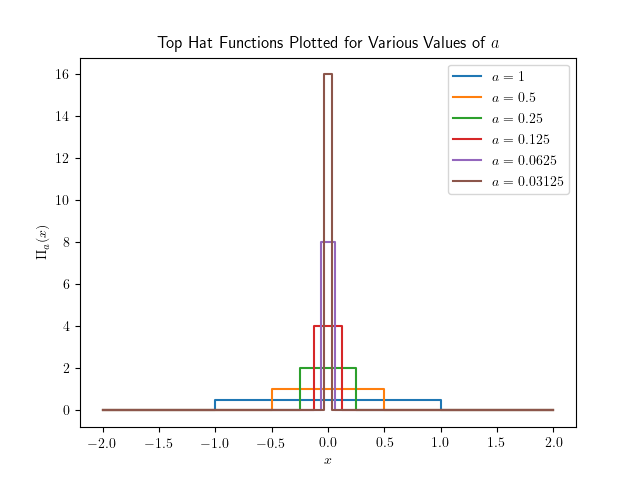
\includegraphics[scale=0.6]{top_hat_function.png}
        \caption{The top hat function, \(\Pi_a\), plotted for various values of \(a\).}
    \end{figure}
    
    Another function that we might consider is the \define{Gaussian}, \(N_\sigma\colon\reals\to\reals\), defined by
    \[N_\sigma(x) = \frac{1}{\sqrt{2\pi\sigma^2}}\exp\left(-\frac{x^2}{2\sigma^2}\right).\]
    This is already normalised so that for all \(\sigma\) we have
    \[\int_{-\infty}^{\infty} \dd x\,N_\sigma = 1.\]
    Again as the `width' (standard deviation, \(\sigma\)) decreases the height increase and in the limit we have
    \[\lim_{\sigma \to 0} N_\sigma(x) = \delta(x).\]
    And as with the top hat function we can choose to centre the delta distribution at \(x = d\) by translating:
    \[\lim_{\sigma \to 0} N_\sigma(x - d) = \delta(x - d).\]
    
    \begin{figure}[ht]
        \centering
        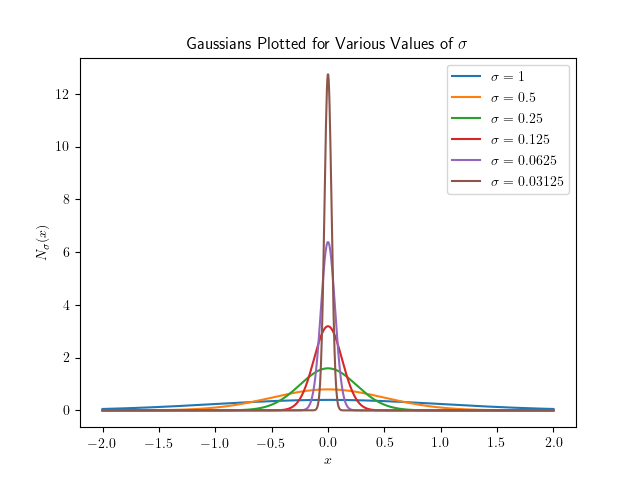
\includegraphics[scale=0.6]{gaussian_function.png}
        \caption{The Gaussian function, \(N_\sigma\), plotted for various values of \(\sigma\).}
    \end{figure}
    
    \subsubsection{Sifting Property}\label{sec:sifting property dirac delta}
    Perhaps the most important property of the Dirac delta is its ability to pick out the value of a function at one point.
    Let \(f\colon\reals\to\reals\) be a function.
    Then
    \[\int_{-\infty}^{\infty} \dd x\,\delta(x - d)f(x) = f(d).\]
    Intuitively this happens because the integrand is zero everywhere apart from at \(x = d\) so this is the only part that contributes to the integral.
    We can show this property occurring more formally using the limit of the top hat function defined above.
    \begin{align*}
        \int_{-\infty}^{\infty} \dd x\,\delta(x - d)f(x) &= \int_{-\infty}^{\infty} \dd x\, f(x)\lim_{a \to 0}\Pi_a(x - d)\\
        &= \lim_{a \to 0}\int_{-\infty}^{\infty} \dd x\, f(x)\Pi_a(x - d)\\
        &= \lim_{a \to 0}\frac{1}{2a}\int_{-a - d}^{a - d} \dd x\, f(x)
    \end{align*}
    We used the fact that the limit is with respect to \(a\) and the integral is with respect to \(x\) to swap the order of the limit and integral.
    We then used the fact that \(\Pi_a(x - d)\) is zero outside of \([-a-d, a-d]\) to change the limits.
    We now identify that
    \[\expected{f(x)} = \frac{1}{2a}\int_{-a-d}^{a-d} \dd x\, f(x)\]
    is the average value of \(x\) over the interval \([-a-d, a-d]\).
    In the limit this interval becomes, \([-d, -d] = \{d\}\), and the average of a function at only one point is just the function evaluated at that point.
    That is \(f(d)\).
    
    Compare this sifting property of the Dirac delta with the analogous, discrete, Kronecker delta:
    \[\sum_{i=1}^n A_i\delta{ij} = A_j.\]
    The Kronecker delta picks out one particular component in the same way that the the Dirac delta picks out the value of a function at one point.\footnote{Viewing the function \(f\) as members of a infinite dimensional vector space of functions with components given by \(f(x)\) these two deltas are actually the same.}
    
    \subsection{Fourier Series}
    In 1822 Joseph Fourier wrote a book called \textit{The Analytical Theory of Heat} in which he claimed that any function can be expanded as a series of sines or cosines:
    \begin{equation}\label{eqn:superposition of waves}
        f(x) = \sum_{n = 0}^\infty A_n\cos(k_nx + \varphi_n).
    \end{equation}
    Such cosines can be viewed as waves with amplitude \(A_n\), wave number \(k_n = 2\pi/\lambda_n\), wave length \(\lambda_n\), and phase \(\varphi_n\).
    While Fourier's claim that all functions can be represented this way isn't actually quite true most functions that we use day to day can be.
    
    The series in equation~\ref{eqn:superposition of waves} is not the standard way to write a \acrfull{fs}.
    The trig identity,
    \[\cos(A + B) = \cos(A)\cos(B) - \sin(A)\sin(B),\]
    can be used to rewrite each term:
    \begin{align*}
        A_n\cos(k_nx + \varphi_n) &= A_n\cos(k_nx)\cos(\varphi_n) - A_n\sin(k_nx)\sin(\varphi_n)\\
        &= a_n\cos(k_nx) + b_n\sin(k_nx)
    \end{align*}
    where we have used the fact that \(\cos(\varphi_n)\) and \(\sin(\varphi_n)\) are just constants for each value of \(n\) and have defined two new constants
    \[a_n = A_n\cos(\varphi_n),\qquad\text{and}\qquad b_n = -A_n\sin(\varphi_n).\]
    Hence the function can be expressed as
    \[f(x) = \sum_{n=0}^\infty a_n\cos(k_nx) + \sum_{n=0}^\infty b_n\sin(k_nx).\]
    This is nice because the phases of all functions in the sums are zero.
    This is still not quite the standard form of a \acrshort{fs} but it is close.
    Before we find the exact form we need to talk about periodic functions.
    
    \subsubsection{Periodic Functions}
    A function, \(f\colon\reals\to\reals\) is periodic with period \(T\) if
    \[f(t + T) = f(t)\]
    for all \(t\in\reals\).
    If \(f\) is periodic with period \(T\) then \(f\) is also periodic with period \(nT\) for all \(n\in\integers\).
    The smallest, positive, value of \(T\) such that \(f\) is periodic with period \(T\) is called the fundamental period of \(f\).
    Note that this definition doesn't require \(f\) to be continuous.
    Consider \(f\) defined by \(f(x) = \{x\} = x - \lfloor x \rfloor\), which gives just the fractional part of \(x\).
    For example, \(f(1.5) = 0.5\), \(f(\pi) = 0.1415926\dots\).
    This function is periodic with fundamental period 1 but is discontinuous everywhere in \(\integers\).
    
    \begin{figure}[ht]
        \centering
        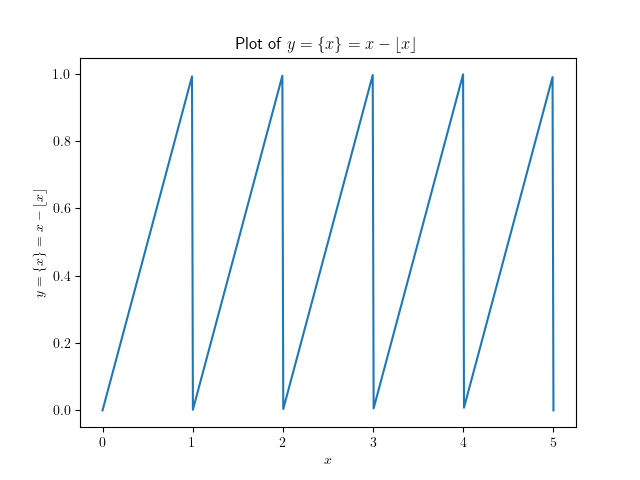
\includegraphics[scale=0.6]{sawtooth.png}
        \caption{Plot of \(y = \{x\} = x - \lfloor x \rfloor\), showing it is periodic with fundamental period 1 and also discontinuous at all \(n\in\integers\).}
    \end{figure}
    
    The set, \(P_T\) of periodic functions, \(f\colon\reals\to\reals\), with period \(T\) forms a vector space under function addition and scalar multiplication, as well as being closed under function multiplication.
    These operations are defined as follows:
    \[(cf)(t) = c[f(t)],\qquad (f + g)(t) = f(t) + g(t),\qquad\text{and}\qquad (fg)(t) = f(t)g(t),\]
    where \(c\in\reals\) and \(f, g\in P_T\)
    It is fairly simple to show that the set of periodic functions with period \(T\) is closed under these operations:
    \[(cf)(t + T) = c[f(t + T)] = c[f(t)] = (cf)(t),\]
    \[(f + g)(t + T) = f(t + T) + f(t + T) = f(t) + g(t) = (f + g)(t),\]
    and
    \[(fg)(t + T) = f(t + T)g(t + T) = f(t)g(t) = (fg)(t).\]
    These hold for all \(t\) so we conclude that \((cf), (f + g), (fg)\in P_T\).
    
    The fundamental period of \(\cos(x)\) and \(\sin(x)\) is \(2\pi\).
    Using this we find that the fundamental period of \(\cos(n\pi x/L)\) and \(\sin(n\pi x/L)\) is \(2L/n\), it is simple to show that this is period, we will do it here for \(\cos\) only:
    \[\cos\left(\frac{n\pi (x + 2L/n)}{L}\right) = \cos\left(\frac{n\pi x}{L} + \frac{n\pi2L/n}{L}\right) = \cos\left(\frac{n\pi x}{L} + 2\pi\right) = \cos\left(\frac{n\pi x}{L}\right).\]
    Note that the period is added to \(x\), not the whole argument of \(\cos\).
    
    \subsubsection{Fourier Expansion}
    Fourier series deal with functions that are periodic over a finite interval, for example \([-1, 1]\), outside this interval the function is assumed to repeat.
    This means that \acrshort{fs} are useful if a. the function really does repeat outside this interval, that is it is periodic with period equal to the length of the interval, or b. we only care about the function in the interval, for example a string attached at \(x = 0\) and \(x = \ell\), we don't care what happens outside \([0, \ell]\).
    If we need the whole domain of the function then we can use a \acrfull{ft}, which we will discuss in a later section.
    
    We can decompose any function in this way, as long as some mild mathematical restrictions are satisfied.
    The sines and cosines that we use are said to form a complete set.
    That is they form a basis set for the vector space of functions.
    There are other complete sets that we could choose, for example powers of \(x\), we do this when using Taylor series.
    
    The standard way to write the \define{\acrfull{fs}} for a function, \(f\colon\reals\to\reals\), over the interval \([-L, L]\), is
    \begin{align*}
        f(x) &= \frac{1}{2}a_0 + \sum_{n=1}^\infty\cos\left(\frac{n\pi x}{L}\right) + \sum_{n=1}^\infty b_n\sin\left(\frac{n\pi x}{L}\right)\\
        &= \frac{1}{2}a_0 + \sum_{n=1}^\infty\left[a_n\cos\left(\frac{n\pi x}{L}\right) + b_n\sin\left(\frac{n\pi x}{L}\right)\right]
    \end{align*}
    where \(a_n, b_n\in\reals\) are called the \define{expansion coefficients}, or \define{Fourier components}.
    The reason for the factor of \(1/2\) in the \(a_0\) term is explained later.
    
    \subsubsection{What about nonpositive \texorpdfstring{\(n\)}{n}?}
    Why do we restrict ourselves to \(n > 0\)?
    Lets see what happens if we don't.
    Suppose that \(f\colon\reals\to\reals\) is a function that we can express as a \acrshort{fs} with expansion coefficients \(A_n\) and \(B_n\) where \(n\in\integers\).
    Then
    \begin{align*}
        f(x) &= \sum_{n\in\integers}\left[A_n\cos\left(\frac{n\pi x}{L}\right) + B_n\sin\left(\frac{n\pi x}{L}\right)\right]\\
        &= A_0\cos\left(\frac{0\pi x}{L}\right) + B_0\sin\left(\frac{0\pi x}{L}\right) + \sum_{n=1}^\infty\left[A_n\cos\left(\frac{n\pi x}{L}\right) + A_{-n}\cos\left(\frac{-n\pi x}L{}\right)\right.\\
        &\left.\qquad+ B_n\sin\left(\frac{n\pi x}{L}\right) + B_{-n}\sin\left(\frac{-n\pi x}{L}\right)\right]\\
        &= A_0\cos(0) + B_0\sin(0) + \sum_{n=1}^\infty\left[A_n\cos\left(\frac{n\pi x}{L}\right) + A_{-n}\cos\left(\frac{n\pi x}L{}\right)\right.\\
        &\left.\qquad+ B_n\sin\left(\frac{n\pi x}{L}\right) - B_{-n}\sin\left(\frac{n\pi x}{L}\right)\right]\\
        &= A_0\cdot 1 + B_0\cdot 0 + \sum_{n=1}^\infty\left[(A_n + A_{-n})\cos\left(\frac{n\pi x}{L}\right) + (B_n - B_{-n})\sin\left(\frac{n\pi x}{L} \right)\right]\\
        &= A_0 + \sum_{n=1}^\infty\left[(A_n + A_{-n})\cos\left(\frac{n\pi x}{L}\right) + (B_n - B_{-n})\sin\left(\frac{n\pi x}{L}\right)\right]\\
        &= \frac{1}{2}a_0 + \sum_{n=1}^\infty\left[a_n\cos\left(\frac{n\pi x}{L}\right) + b_n\sin\left(\frac{n\pi x}{L}\right)\right].
    \end{align*}
    Here we define \(A_0 = a_0/2\), \(a_n = A_n + A_{-n}\), and \(b_n = B_n - B_{-n}\) for \(n\in\integers^+\).
    So we see that if we do include negative values of \(n\) they can simply be hidden away, similarly the term that would have \(b_0\) just happens to be zero as \(\sin(0) = 0\).
    Again the factor of \(1/2\) will be explained when we look at how to compute \(a_n\) and \(b_n\).
    
    \section{Orthogonality}
    The functions \(\cos(k_ix)\) and \(\sin(k_ix)\) for \(i\in\integers_{>0}\) form an \define{orthogonal basis}.
    By this we mean
    \begin{align*}
        \int_{-L}^{L} \dd{x}\cos\left(\frac{m\pi x}{L}\right) \cos\left(\frac{n\pi x}{L}\right) &= 
        \begin{cases}
            0, & m \ne n,\\
            L, & m = n,
        \end{cases}
        = L\delta_{mn}\\
        \int_{-L}^{L} \dd{x}\sin\left(\frac{m\pi x}{L}\right) \sin\left(\frac{n\pi x}{L}\right) &= 
        \begin{cases}
            0, & m \ne n,\\
            L, & m = n,
        \end{cases}
        = L\delta_{mn}\\
        \int_{-L}^{L} \dd{x}\cos\left(\frac{m\pi x}{L}\right)\sin\left(\frac{n\pi x}{L}\right) &= 0
    \end{align*}
    We also have a constant term for one of the Fourier nodes (the \(a_0/2\) term).
    This means we also need
    \begin{align*}
        \int_{-L}^{L} \dd{x} \cos\left(\frac{n\pi x}{L}\right) &= 
        \begin{cases}
            0, &n \ne 0,\\
            2L, &n = 0,
        \end{cases}
        = 2L\delta_{m0}\\
        \int_{-L}^{L} \dd{x} \sin\left(\frac{n\pi x}{L}\right) &= 0
    \end{align*}
    Note the extra factor of 2 here as opposed to the case of two cosine functions.
    We will show that the first of these equations holds and the others follow in much that same way.
    To do this we use the following identity:
    \[\cos(A)\cos(B) = \frac{1}{2}\left[\cos(A + B) + \cos(A - B)\right].\]
    This is easily shown by adding the identities for addition and subtraction of angles.
    Applying this gives us
    \begin{align*}
        I &= \int_{-L}^{L} \dd{x} \cos\left(\frac{m\pi x}{L}\right) \cos\left(\frac{n\pi x}{L}\right)\\
        &= \underbrace{\frac{1}{2} \int_{-L}^{L} \dd{x} \cos\left([m + n]\frac{\pi x}{L}\right)}_{= I_1} + \underbrace{\frac{1}{2} \int_{-L}^L \dd{x} \cos\left([m - n]\frac{\pi x}{L}\right)}_{= I_2}
    \end{align*}
    Looking at the first integral we have
    \begin{align*}
        I_1 &= \frac{1}{2} \int_{-L}^L \dd{x} \cos\left([m + n]\frac{\pi x}{L}\right)
        \shortintertext{Making the substitution \(\vartheta = \pi x/L\), so \(x = \vartheta L/\pi\) we get \(\dd{\vartheta} = \pi\dd{x}/L\) and the integral goes from \(x\in[-L, L]\) to \(\vartheta\in[-\pi, \pi]\):}
        &= \frac{1}{2}\int_{-\pi}^{\pi} \dd{\vartheta} \frac{L}{\pi} \cos([m + n]\vartheta)\\
        &= \frac{L}{2\pi}\int_{-\pi}^{\pi} \dd{\vartheta} \cos([m + n]\vartheta)\\
        &= \frac{L}{2\pi}\left[\frac{1}{m + n}\sin([m + n]\vartheta)\right]_{-\pi}^{\pi}\\
        &= 0
    \end{align*}
    where we have used the fact that \(\sin(k\pi) = 0\) for all \(k\in\integers\) and clearly \([m + n]\in\integers\).
    
    Looking now at the second integral we can use exactly the same logic but with \([m + n]\) replaced with \([m - n]\).
    This gets us to
    \begin{align*}
        I_2 &= \frac{1}{2}\int_{-L}^{L} \dd{x} \cos\left([m - n]\frac{\pi x}{L}\right)\\
        &= \frac{L}{2\pi} \frac{1}{m - n} \left[\sin([m - n]\vartheta)\right]_{-\pi}^{\pi}\\
        &= \frac{L}{2\pi} \frac{1}{m - n} \left[\sin([m - n]\pi) - \sin(-[m - n]\pi)\right]\\
        &= \frac{L}{2\pi} \frac{1}{m - n} \left[\sin([m - n]\pi) + \sin([m - n]\pi)\right]\\
        &= \frac{L}{\pi} \frac{1}{m - n} \sin([m -n]\pi)\\
    \end{align*}
    We now have to consider two cases.
    The first is that \(m \ne n\).
    In this case we have \(0 \ne m - n \in\integers\) and so \(\sin([m - n]\pi) = 0\).
    Thus the whole integral is zero: \(I_2 = 0\).
    The second case is that \(m = n\).
    In this case we have \(m - n = 0\) which means that our integral is indeterminate of the form \(0/0\) as we have \(\sin(0) = 0\) in the numerator and \(m - n = 0\) in the denominator.
    Fortunately we can find the correct limit easily by avoiding this indeterminate form entirely and looking at the original integral in this specific case:
    \begin{align*}
        I_2 &= \frac{1}{2} \int_{-L}^{L} \dd{x} \cos\left([m - n]\frac{\pi x}{L}\right)\\
        &= \frac{1}{2} \int_{-L}^{L} \dd{x} \cos(0)\\
        &= \frac{1}{2} \int_{-L}^{L} \dd{x}\\
        &= L.
    \end{align*}
    Thus we have
    \begin{align*}
        I = I_1 + I_2 = I_2 = \delta_{mn}L.
    \end{align*}
    
    \subsection{Finding Fourier Series Coefficients}
    We can use the orthogonality of these functions to find the Fourier coefficients.
    Let \(f\) be a function that can be expressed as a Fourier series as
    \[f(x) = \frac{a_0}{2} + \sum_n a_n\cos\left(\frac{n\pi x}{L}\right) + \sum_n b_n\sin\left(\frac{n\pi x}{L}\right).\]
    To find \(a_n\) we compute
    \begin{align*}
        I &= \int_{-L}^{L} \dd{x} \cos\left(\frac{m\pi x}{L}\right)f(x)\\
        &= \int_{-L}^{L} \dd{x} \cos\left(\frac{m\pi x}{L}\right)\frac{a_0}{2} + \int_{-L}^{L} \dd{x} \cos\left(\frac{m\pi x}{L}\right)\sum_n a_n\cos\left
        (\frac{n\pi x}{L}\right)\\
        &\qquad + \int_{-L}^{L} \dd{x} \cos\left(\frac{m\pi x}{L}\right) \sum_n b_n\sin\left(\frac{n\pi x}{L}\right)\\
        &= \frac{a_0}{2}\int_{-L}^{L} \dd{x} \cos\left(\frac{m\pi x}{L}\right) + \sum_n a_n \int_{-L}^{L} \dd{x} \cos\left(\frac{m\pi x}{L}\right) \cos\left(\frac{n\pi x}{L}\right)\\
        &\qquad + \sum_n b_n \int_{-L}^{L} \dd{x} \cos\left(\frac{m\pi x}{L}\right) \sin\left(\frac{n\pi x}{L}\right)\\
        &= \frac{a_0}{2}2L\delta_{m0} + \sum_n a_n L\delta_{mn} + \sum_n b_n\cdot 0\\
        &= a_0L\delta_{m0} + L\sum_n a_n\delta_{mn}.
    \end{align*}
    We now consider two cases.
    First \(m \ne 0\), then \(\delta_{m0} = 0\) so \(I = a_mL\).
    Next \(m = 0\), in this case the second term is actually zero as \(n\in\integers_{>0}\) so \(n \ne 0 = m\) so \(\delta_{mn} = 0\) and we get \(I = a_0L\delta_{m0} = a_0L\).
    Thus by simply rearranging we have
    \[a_m = \frac{1}{L}\int_{-L}^{L} \dd{x}\cos\left(\frac{m\pi x}{L}\right)f(x).\]
    This works for \(m = 0\) or \(m > 0\), this is why we include the factor of \(1/2\) with the \(a_0\) term, so we can use the same formula for all \(a\) coefficients.
    
    We can show in a similar way that
    \[b_m = \frac{1}{L}\int_{-L}^{L} \dd{x} \sin\left(\frac{m\pi x}{L}\right)f(x).\]
    
    \subsection{Even and Odd Functions}
    A function, \(f\), is \define{even} if \(f(-x) = f(x)\), similarly \(f\) is \define{odd} if \(f(-x) = -f(x)\).
    These are important properties as if \(f\) is even or odd it makes finding its Fourier series a lot easier:
    \begin{itemize}
        \item If \(f\) is even then \(b_m = 0\) and
        \[a_m = \frac{1}{L} \int_{-L}^{L} \dd{x} \cos\left(\frac{m\pi x}{L}\right) = \frac{2}{L} \int_{0}^{L} \cos\left(\frac{m\pi x}{L}\right).\]
        \item If \(f\) is odd then \(a_m = 0\) and
        \[b_m = \frac{1}{L} \int_{-L}^{L} \dd{x} \sin\left(\frac{m\pi x}{L}\right) = \frac{2}{L} \int_{0}^{L} \sin\left(\frac{m\pi x}{L}\right).\]
    \end{itemize}
    Let \(f\) be an even function.
    Then
    \[I = \int_{-L}^{L} \dd{x} f(x) = \underbrace{\int_{-L}^{0}\dd{x} f(x)}_{= I_1} + \underbrace{\int_{0}^{L} \dd{x} f(x)}_{= I_2}\]
    \begin{align*}
        I_1 &= \int_{-L}^{0} \dd{x} f(x)
        \shortintertext{Making a substitution \(y = -x\) so \(\dd{x} = -\dd{y}\) and the integrals goes from \(x\in[-L, 0]\) to \(y\in[L, 0]\):}
        &= -\int_{L}^{0} \dd{y} f(-y)\\
        &= \int_{0}^{L} \dd{y} f(-y)\\
        &= \int_{0}^{L} \dd{y} f(y)\\
        &= I_2
    \end{align*}
    So we have
    \[I = \int_{-L}^{L} \dd{x} f(x) = I_1 + I_2 = 2I_2 = 2\int_{}^{L} \dd{x} f(x).\]
    Now let \(g\) be an odd function.
    Then
    \[J = \int_{-L}^{L} \dd{x} g(x) = \underbrace{\int_{-L}^{0} \dd{x} g(x)}_{= J_1} + \underbrace{\int_{0}^{L} \dd{x} g(x)}_{= J_2}\]
    \begin{align*}
        J_1 &= \int_{-L}^{0} \dd{x} g(x)\\
        \shortintertext{Making a substitution \(y = -x\) so \(\dd{x} = -\dd{y}\) and the integrals goes from \(x\in[-L, 0]\) to \(y\in[L, 0]\):}
        &= -\int_{L}^{0} \dd{y} g(-y)\\
        &= \int_{0}^{L} \dd{y} g(-y)\\
        &= -\int_{0}^{L} \dd{y} g(y)\\
        &= -J_2
    \end{align*}
    So we have
    \[J = \int_{-L}^{L} \dd{x} g(x) = J_1 + J_2 = -J_2 + J_2 = 0.\]
    Let \(f\) and \(g\) be even functions, then
    \[(fg)(-x) = f(-x)g(-x) = f(x)g(x) = (fg)(x)\]
    using the properties of \(f\) and \(g\) as even functions.
    This means that the function \(fg\) is even.
    Let \(f\) be an even function and \(g\) be an odd function, then
    \[(fg)(-x) = f(-x)g(-x) = f(x)[-g(x)] = -f(x)g(-x) = -(fg)(x)\]
    using the properties of \(f\) as an even function and \(g\) as an odd function.
    This means that the function \(fg\) is odd.
    Finally let \(f\) and \(g\) be odd functions, then
    \[(fg)(-x) = f(-x)g(-x) = [-f(x)][-g(x)] = f(x)g(x) = (fg)(x)\]
    using the properties of \(f\) and \(g\) as odd functions.
    This means that \(fg\) is an odd function.
    So the product of two functions is even if both functions are even or both functions are odd and is odd if only one of the functions is even and the other is odd.
    We can use this to show that the Fourier series of \(f\) do simplify if \(f\) is even or odd.
    The last thing that we need is that \(\cos\) is an even function and \(\sin\) is an odd function.
    
    Let \(f\) be an even function.
    Then
    \[b_m = \frac{1}{L}\int_{-L}^{L} \dd{x} \sin(k_mx)f(x) = 0\]
    as \(f(x)\sin(k_mx)\) is odd.
    Similarly
    \[a_m = \frac{1}{L}\int_{-L}^{L} \dd{x} \cos(k_mx)f(x) = \frac{2}{L}\int_{0}^{L} \cos(k_mx)f(x)\]
    as \(f(x)\cos(k_mx)\) is even.
    We can do the same if \(f\) is an odd function.
    
    \subsection{Vectors}\label{sec:vectors}
    This should all seem similar from basic vector operations.
    It turns out that the set of square integrable functions, \(f\colon\reals\to\reals\), defined on the interval \([-L, L]\) is a vector space. 
    Confusingly the vector space of square integrable functions on \([a, b]\) is usually denoted \(L^2([a, b])\) which means that we are looking at the vector space \(L^2([L, -L])\), which is confusing notation so we will just call this vector space \(F\). 
    Vector addition in \(F\) is defined by
    \[(f + g)(x) = f(x) + g(x)\]
    for all \(x\in[-L, L]\), with \(f, g\in F\).
    Scalar multiplication is defined as
    \[(cf)(x) = c[f(x)]\]
    for all \(x\in[-L, K]\), with \(c\in\reals\) and \(f\in F\).
    
    The square integrable part of this definition simply means that
    \[\int_{-L}^{L} \dd{x} |f(x)|^2\]
    exists and is finite.
    This is important because we define an inner product on this vector space to be
    \[\innerproduct{f}{g} = \int_{-L}^{L} \dd{x} f(x)g(x)\]
    for \(f, g\in F\) and the condition of square integrability ensures that this is well defined.
    If we define \(c_m(x) = \cos(k_mx)\) and \(s_m(x) = \sin(k_mx)\) then the orthogonality condition becomes
    \begin{align*}
        \innerproduct{c_m}{c_n} &= L\delta_{mn}\\
        \innerproduct{s_m}{s_n} &= L\delta_{mn}\\
        \innerproduct{c_m}{s_n} &= 0.
    \end{align*}
    The set of all \(c_m\) and \(s_m\) form an orthogonal basis of \(F\).
    Similarly we can find the Fourier coefficients of the function \(f\) with
    \begin{align*}
        a_m &= \frac{1}{L}\innerproduct{c_m}{f}\\
        b_m &= \frac{1}{L}\innerproduct{s_m}{f}.
    \end{align*}
    This is completely analogous to how in Euclidean three-space, \(\reals^3\), we have that two basis vectors, \(\ve{i}\) and \(\ve{j}\), are orthonormal if \(\ve{i}\cdot\ve{j} = \delta_{ij}\).
    As well as calculating the component \(v_i\) of \(\vv{v}\in\reals^3\) by \(\ve{i}\cdot\vv{v}\).
    
    \section{Periodic Extensions and Complex Fourier Series}
    Let \(f\colon\reals\to\reals\) be a function.
    We can define its Fourier series as \(f_\FS\colon[-L, L]\to\reals\).
    The expansion is only valid for \(x\in[-L, L]\), that is we are only guaranteed that \(f(x) = f_\FS(x)\) if \(x\in[-L, L]\).
    Outside of this interval, while we can extend \(f_\FS\) to be defined on all \(\reals\), this is called the periodic expansion of \(f_\FS\).
    There is no guarantee that the periodic expansion will be equal to \(f\) outside of \([-L, L]\).
    For example if \(f\) is not periodic then \(f_\FS\) extended to all \(x\in\reals\) is periodic with period \(2L\) therefore it cannot be equal to \(f\).
    Similarly it could be that \(f\) has discontinuities outside of \([-L, L]\) but \(f_\FS\) is a sum of continuous functions so must be continuous.
    Again this stops us having equality between \(f\) and \(f_\FS\) everywhere.
    
    Consider the function \(f\colon\reals\to\reals\), \(f(x) = x^2\).
    Clearly this is an even function so its Fourier series has only cosine components with coefficients given by
    \[a_n = \frac{2}{L} \int_{0}^{L} \dd{x} x^2 \cos\left(\frac{n\pi x}{L}\right) = \frac{2}{L}I_n.\]
    The integrals can be computed as follows:
    \[I_n = \int_0^L \dd{x} x^2 \cos\left(\frac{n\pi x}{L}\right).\]
    Now integrate by parts.
    \[
        \begin{array}{ll}
            u = x^2, & v = \frac{L}{n\pi}\sin\left(\frac{n\pi x}{L}\right),\\[0.5em]
            u' = 2x, & v' = \cos\left(\frac{n\pi x}{L}\right),
        \end{array}
    \]
    assuming that \(n \ne 0\).
    \begin{align*}
        I_n &= \left[\frac{L}{n\pi}x^2\sin\left(\frac{n\pi x}{L}\right)\right]_0^L - \frac{2L}{n\pi}\int_0^L \dd{x} x\sin\left(\frac{n\pi x}{L}\right)\\
        &= \frac{L}{n\pi}L^2\sin(n\pi) - \frac{2L}{n\pi}\int_0^L \dd{x} x\sin\left(\frac{n\pi x}{L}\right)\\
        &= -\frac{2L}{n\pi}\int_0^L \dd{x} x\sin\left(\frac{n\pi x}{L}\right)
    \end{align*}
    Integrating by parts again
    \[
        \begin{array}{ll}
            u = x  & v = -\frac{L}{n\pi}\cos\left(\frac{n\pi x}{L}\right)\\[0.5em]
            u' = 1 & v' = \sin\left(\frac{n\pi x}{L}\right)
        \end{array}
    \]
    \begin{align*}
        I_n &= -\frac{2L}{n\pi}\left[ \left[ -\frac{L}{n\pi} x\cos\left(\frac{n\pi x}{L}\right) \right]_0^L + \frac{L}{n\pi} \int_0^L\dd{x} \cos\left(\frac{n\pi x}{L}\right) \right]\\
        &= -\frac{2L}{n\pi}\left[ -\frac{L}{n\pi}L\cos(n\pi) + \frac{L}{n\pi}\left[ \frac{L}{n\pi}\sin\left(\frac{n\pi x}{L}\right) \right]_0^L \right]\\
        &= \frac{2L^3}{n^2\pi^2}(-1)^n + \frac{L^2}{n^2\pi^2}[\sin(n\pi) - \sin(0)]\\
        &= \frac{2L^3}{n^2\pi^2}(-1)^n.
    \end{align*}
    We also need to consider the case when \(n = 0\), fortunately this is very simple:
    \[I_0 = \int_0^L\dd{x} x^2\cos(0) = \int_0^L x^2 \dd{x} = \frac{1}{3}\left[x\right]_0^L = \frac{L^3}{3}.\]
    Dividing this by two and adding the rest of the terms as well as the constant prefactor of \(2/L\) gives us the Fourier series:
    \begin{align*}
        f_\FS(x) &= \frac{2}{L}\frac{L^3}{3}\frac{1}{2} + \frac{2}{L}\sum_{n=1}^{\infty}\frac{2L^3}{n^2\pi^2}(-1)^n\cos\left(\frac{n\pi x}{L}\right)\\
        &= \frac{1}{3}L^2 + \frac{4L^2}{\pi^2}\sum_{n=1}^{\infty}\frac{(-1)^n}{n^2}\cos\left(\frac{n\pi x}{L}\right).
    \end{align*}
    The periodic expansion of this Fourier series and original function are plotted for comparison in figure~\ref{fig:fourier series x^2}.
    \begin{figure}[ht]
        \centering
        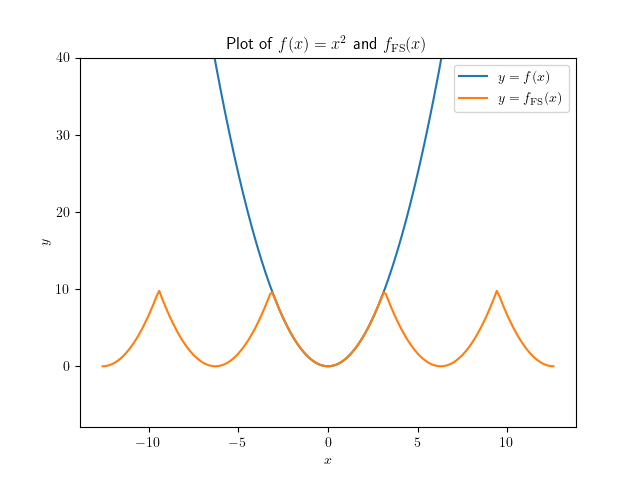
\includegraphics[scale=0.6]{fourier_xsquared.png}
        \caption{Plot of \(f(x) = x^2\) and the periodic expansion of \(f_\FS(x)\). A value of \(L = \pi\) was chosen and the series was computed up to \(n = 1000\).}
        \label{fig:fourier series x^2}
    \end{figure}

    If the Fourier series isn't always equal to the original function why might we want to use it?
    The interval over which \(f(x) = f_\FS(x)\) is called the universe.
    If we are only interested in \(f\) when evaluated in the universe it can be much more efficient to use the Fourier series.
    Consider the example of \(f(x) = (1 + \sin x)^2.\)
    Expanding this gives us
    \[(1 + \sin x)^2 = 1 + 2\sin x + \sin^2x = 1 + 2\sin x + \frac{1}{2}(1 - \cos(2x)) = \frac{3}{2} - \frac{1}{2}\cos(2x) + 2\sin x.\]
    We can simply read off the values of the Fourier coefficients from this:
    \[a_0 = 3,\qquad a_2 = -\frac{1}{2},\qquad\text{and}\qquad b_1 = 2.\]
    All other coefficients are zero.
    This means that we can completely encode this function with just six values, the index of each coefficient that is nonzero and its value.
    In this case this doesn't save much space or speed things up much but the more complicated \(f\) is the more efficient it becomes to use the Fourier series.
    This does only give us a finite level of precision if we need an infinite number of terms but we simply use enough that we have the desired level of precision.
    
    If our original function had instead been \(f\colon\reals_{\ge 0}\to\reals\), \(f(x) = x^2\) then we are left with an interesting choice.
    One time when this might be the case is if \(f\) is a function of time and we know something increases quadratically after a start point but don't care what happened before that.
    We need to somehow extend \(f\) to be defined on \([-L, 0]\) as well to compute the Fourier series.
    The choice of how we do this is up to us if we don't care about \(f\) at \(x < 0\).
    There are two logical ways to do it.
    We could either make \(f\) and even function or we could make \(f\) an odd function.
    If we make it an even function we just end up defining \(f_\text{even}\colon\reals\to\reals\), \(f_\text{even}(x) = x^2\).
    We already computed the Fourier series for this.
    If instead we choose to make \(f\) an odd function then we get \(f_\text{odd}\colon\reals\to\reals\), \(f_\text{odd}(x) = \sgn(x)x^2\) where
    \[
        \sgn(x) = 
        \begin{cases}
            1, & x > 0,\\
            0, & x = 0,\\
            -1, & x < 0.
        \end{cases}
    \]
    These are plotted in figure~\ref{fig:extension of x^2 defined on x>0}.
    \begin{figure}[ht]
        \centering
        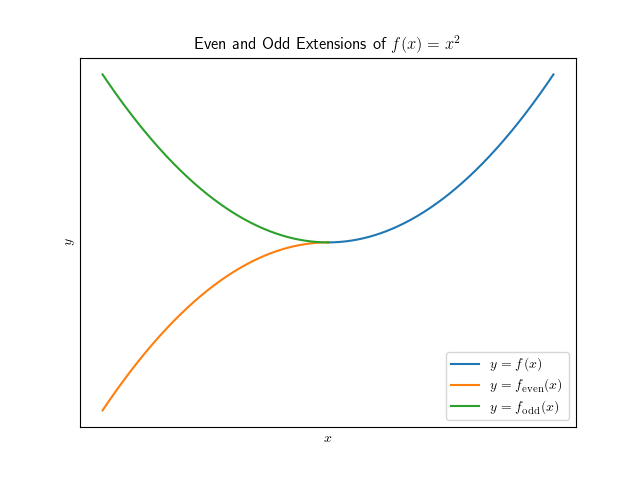
\includegraphics[scale=0.6]{extensions_of_xsquared.png}
        \caption{\(f(x) = x^2\) extended to negative values of \(x\) in two different ways.}
        \label{fig:extension of x^2 defined on x>0}
    \end{figure}
    We can compute the Fourier expansion of \(f_\text{odd}\) as well.
    Since it is an odd function its Fourier series has only sine components with coefficients
    \[b_m = \frac{2}{L}\int_0^L \dd{x} \sgn(x)x^2\sin\left(\frac{n\pi x}{L}\right) = \frac{2}{L}I_n.\]
    Helpfully for \(x\in(0, L]\) \(\sgn(x) = 1\) and \(\sgn(0) = 0\) so for \(x\in[0, L]\) \(\sgn(x)x^2 = x^2\).
    Hence
    \[I_n = \int_0^L \dd{x} x^2 \sin\left(\frac{n\pi x}{L}\right).\]
    We can integrate this by parts:
    \[
        \begin{array}{ll}
            u = x^2, & v = -\frac{L}{n\pi}\cos\left(\frac{n\pi x}{L}\right),\\[0.5em]
            u' = 2x, & v' = \sin\left(\frac{n\pi x}{L}\right).
        \end{array}
    \]
    \begin{align*}
        I_n &= \left[-\frac{L}{n\pi}x^2\cos\left(\frac{n\pi x}{L}\right)\right]_0^L + \frac{L}{n\pi} \int_0^L \dd{x} x\cos\left(\frac{n\pi x}{L}\right)\\
        &= -\frac{L}{n\pi}L^2\cos(n\pi) + \frac{L}{n\pi} \int_0^L \dd{x} x\cos\left(\frac{n\pi x}{L}\right)\\
        &= \frac{L}{n\pi}\left[-L^2(-1)^n + \int_0^L \dd{x} x\cos\left(\frac{n\pi x}{L}\right)\right]\\
        &= \frac{L}{n\pi}\Bigg[L^2(-1)^{n+1} + \underbrace{\int_0^L \dd{x} x\cos\left(\frac{n\pi x}{L}\right)}_{=I_n'}\Bigg].
    \end{align*}
    We can integrate \(I_n'\) by parts:
    \[
        \begin{array}{ll}
            u = x,  & v = \frac{L}{n\pi}\sin\left(\frac{n\pi x}{L}\right),\\[0.5em]
            u' = 1, & v' = \cos\left(\frac{n\pi x}{L}\right).
        \end{array}
    \]
    \begin{align*}
        I_n' &= \left[\frac{L}{n\pi}x\sin\left(\frac{n\pi x}{L}\right)\right]_0^L - \frac{L}{n\pi}\int_0^L \dd{x} \sin\left(\frac{n\pi x}{L}\right)\\
        &= -\frac{L}{n\pi}\left[-\frac{L}{n\pi}\cos\left(\frac{n\pi x}{L}\right)\right]_0^L\\
        &= \frac{L^2}{n^2\pi^2}[\cos(n\pi) + \cos(0)]\\
        &= \frac{L^2}{n^2\pi^2}[(-1)^n + 1].
    \end{align*}
    Substituting this back into \(I_n\) gives us
    \begin{align*}
        I_n &= \frac{L}{n\pi}\left[(-1)^{n+1}L^2 + \frac{L^2}{n^2\pi^2}[(-1)^n + 1]\right]\\
        &= \frac{L^3}{n^3\pi^3}[n^2\pi^2(-1)^{n+1} + (-1)^n + 1]
    \end{align*}
    This gives the Fourier coefficients as
    \[b_m = \frac{2L^2}{n^3\pi^3}[n^2\pi^2(-1)^{n+1} + (-1)^n + 1].\]
    Thus the full Fourier series is
    \[f_{\text{odd},\FS}(x) = \frac{2L^2}{\pi^3}\sum_n \frac{1}{n^3}[n^2\pi^2(-1)^{n+1} + (-1)^n + 1]\sin\left(\frac{n\pi x}{L}\right).\]
    This is plotted along with \(f(x) = x^2\) in figure~\ref{fig:odd extension of x^2}.
    As you can see despite being cut off at the same number of terms as \(f_{\text{even}, \FS}\) is in figure~\ref{fig:fourier series x^2} the error is much greater.
    You can think of this as \(-\cos(x)\) already being fairly quadratic shaped at \(x = 0\) whereas \(\sin(x)\) is more linear.
    By looking at the two expansions we see that terms in the expansion of \(f_{\text{even}, \FS}\) drop of as \(1/n^2\) whereas terms in \(f_{\text{odd}, \FS}\) drop of as \(1/n\) meaning we need to include more terms to have the error be the same.
    \begin{figure}[ht]
        \centering
        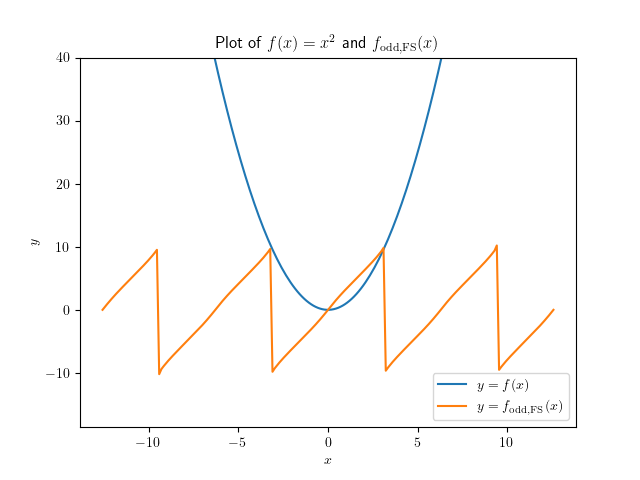
\includegraphics[scale=0.6]{fourier_xsquared_odd.png}
        \caption{Plot of \(f(x) = x^2\) and the periodic expansion of \(f_{\text{odd},\FS}(x)\). A value of \(L = \pi\) was chosen and the series was computed up to \(n = 1000\).}
        \label{fig:odd extension of x^2}
    \end{figure}
    \begin{figure}[ht]
        \centering
        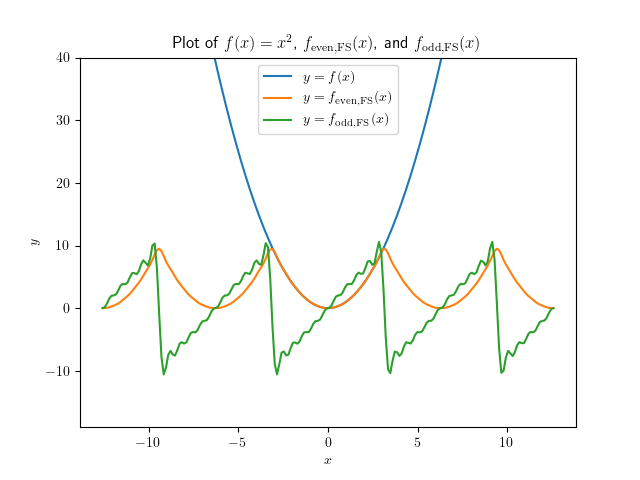
\includegraphics[scale=0.6]{fourier_xsquared_even_and_odd.png}
        \caption{Plot of \(f(x) = x^2\) and the periodic expansions \(f_{\text{even},\FS}(x)\), and \(f_{\text{odd},\FS}(x)\). A value of \(L = \pi\) was chosen and the series was computed up to \(n = 10\).}
    \end{figure}
    One way to judge how quickly a Fourier series converges is to plot the coefficients as a function of \(n\).
    This is called spectral analysis.
    We want them to tend to zero as fast as possible.
    \begin{figure}[ht]
        \centering
        \begin{subfigure}{0.45\textwidth}
            \centering
            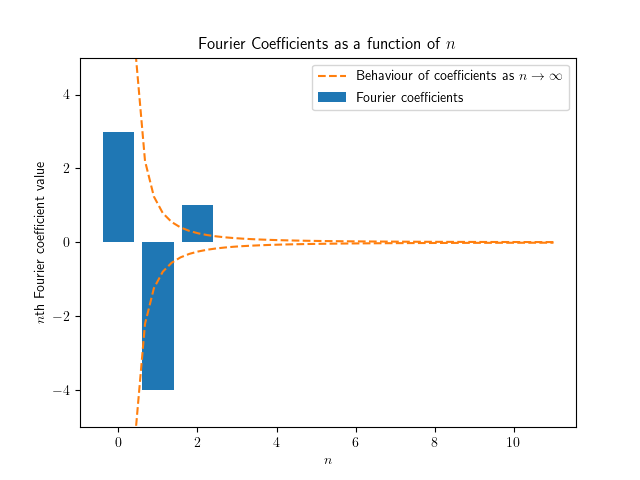
\includegraphics[scale=0.5]{spectral_analysis_xsquared_even.png}
            \caption{Spectral analysis for \(f_{\text{even},\FS}\).}
        \end{subfigure}
        \hspace{3em}
        \begin{subfigure}{0.45\textwidth}
            \centering
            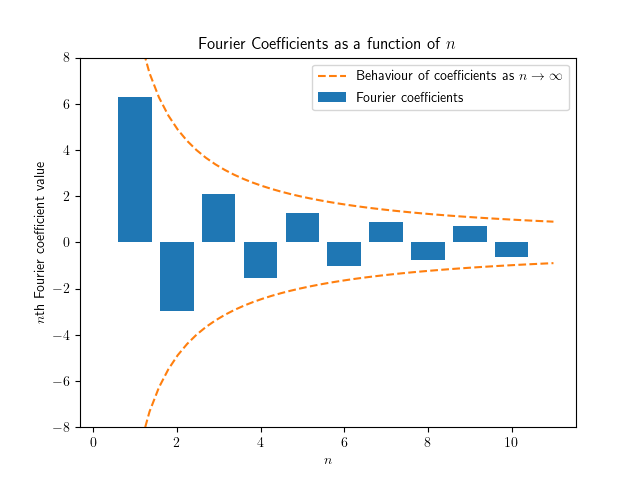
\includegraphics[scale=0.5]{spectral_analysis_xsquared_odd.png}
            \caption{Spectral analysis for \(f_{\text{odd},\FS}\).}
        \end{subfigure}
        \caption{Spectral analysis for the odd and even expansions of \(f(x) = x^2\) showing the behaviour of the coefficients as \(n \to\infty\).}
    \end{figure}
    
    \subsection{Complex Fourier Series}
    So far we have dealt only with real Fourier series, these are characterised by a real function, \(f\colon\reals\to\reals\), which has a real Fourier series \(f_\FS\) with a basis of sines and cosines and coefficients, \(a_n, b_n \in\reals\).
    
    It is also possible to construct a Fourier series for a complex function, \(f\colon\reals\to\complex\).
    This series will have a basis of functions of the form 
    \[\varphi_n(x) = e^{ik_nx} = \exp\left(\frac{in\pi x}{L}\right).\]
    As with the real case \(\{\varphi_n\}\) form an orthogonal basis.
    By this we mean that
    \[
        \int_{-L}^{L}\dd{x}\varphi_n(x)^*\varphi_m(x) = 
        \begin{cases}
            0, & n \ne m,\\
            2L, & n = m,
        \end{cases}
        = 2L\delta_{mn}.
    \]
    This is fairly easy to show:
    \begin{align*}
        I &= \int_{-L}^{L} \dd{x} \varphi_m(x)^*\varphi_n(x)\\
        &= \int_{-L}^{L} \dd{x} \exp\left(-\frac{im\pi x}{L}\right) \exp\left(\frac{in\pi x}{L}\right)\\
        &= \int_{-L}^{L} \dd{x} \exp\left[\frac{i\pi x}{L}[m - n]\right]
        \shortintertext{assuming \(m \ne n\) this gives}
        &= \frac{L}{i\pi(m - n)}\left[\exp\left(\frac{i\pi x}{L}(m - n)\right)\right]_{-L}^{L}\\
        &= \frac{L}{i\pi(m - n)}\left[\exp\left(i\pi(m - n)\right) - \exp\left(-i\pi(m - n)\right)\right]\\
        &= \frac{L}{i\pi(m - n)}\left[(e^{i\pi})^{m-n} - (e^{i\pi})^{n-m}\right]\\
        &= \frac{L}{i\pi(m - n)}\left[(-1)^{m-n} - (-1)^{n-m}\right]\\
        &= 0
    \end{align*}
    In the case that \(m = n\) our integral reduces to
    \begin{align*}
        I &= \int_{-L}^{L} \dd{x} \varphi_m(x)^*\varphi_n(x)\\
        &= \int_{-L}^{L} \dd{x} \exp\left(-\frac{im\pi x}{L}\right) \exp\left(\frac{in\pi x}{L}\right)\\
        &= \int_{-L}^{L} \dd{x} \exp\left[\frac{i\pi x}{L}[m - n]\right]\\
        &= \int_{-L}^{L} \dd{x} e^0\\
        &= 2L
    \end{align*}
    If \(f\colon\reals\to\complex\) is a function then its complex Fourier series is
    \[\sum_{n\in\integers} c_n\varphi_n(x),\]
    where \(c_n\in\complex\).
    Note that we do now have to sum over negative integers as well as there is no way to include these terms in the positive integer ones in the way that we did with real Fourier series.
    We can use the orthogonality condition to find the coefficient \(c_m\):
    \begin{align*}
        \int_{-L}^{L} \dd{x} f(x)\varphi_m(x)^* &= \int_{-L}^{L} \dd{x} \sum_{n\in\integers}c_n\varphi_n(x)\varphi_m(x)^*\\
        &= \sum_{n\in\integers}c_n\int_{-L}^{L} \dd{x} \varphi_m(x)^* \varphi(n)\\
        &= \sum_{n\in\integers}2c_nL\delta_{nm}\\
        &= 2c_mL
    \end{align*}
    so we can identify
    \[c_m = \frac{1}{2L}\int_{-L}^{L}\dd{x}f(x)\varphi_m(x)^*.\]
    
    \subsubsection{Vectors}
    Going back to Fourier series as vectors the set of square integrable functions, \(f\colon\reals\to\complex\), forms a complex vector space.
    Almost everything in section~\ref{sec:vectors} holds but in a complex vector space for \(f, g\colon\reals\to\complex\) the inner product is defined as
    \[\innerproduct{f}{g} = \int_{-L}^{L} \dd{x} f(x)^*g(x).\]
    From this we see that the orthogonality condition is simply
    \[\innerproduct{\varphi_m}{\varphi_n} = 2L\delta_{mn}.\]
    We can find the coefficients using
    \[c_m = \frac{1}{2L}\innerproduct{\varphi_m}{f}.\]
    
    \section{Real and Complex Fourier Series}
    Suppose \(f\colon\reals\to\reals\).
    Then \(f(x) = f^*(x)\) for all \(x\in\reals\).
    We can expand \(f\) as a complex Fourier series:
    \[f(x) = \sum_{n\in\integers}c_ne^{ik_nx}.\]
    Taking the complex conjugate we have
    \begin{align*}
        f^*(x) &= \sum_{n\in\integers}c_n^*e^{-ik_nx}\\
        &= \sum_{n\in\integers}c_n^*e^{-in\pi x/L}\\
        \shortintertext{rename dummy index, \(n\to-n\):}
        f^*(x) &= \sum_{n\in\integers}c_{-n}^*e^{in\pi x/L}\\
        &= \sum_{n\in\integers}c_{-n}^*e^{ik_nx}\\
    \end{align*}
    Now using the fact that \(\{e^{ik_nx}\}\) is an orthogonal basis and \(f(x) = f^*(x)\) we must have that
    \[c_n = c_{-n}^*.\]
    This is a handy check after computing a complex Fourier series for a real valued function.
    This is known as the Hermitian property of \(f\).
    
    \subsection{Relationship Between Real and Complex Fourier Coefficients}
    Let \(f\colon\reals\to\reals\) have a complex Fourier series with Fourier coefficients \(c_n\).
    We can compute \(c_n\) as
    \begin{align*}
        c_n &= \frac{1}{2L}\int_{-L}^{L} \dd{x} f(x)\varphi_n^*(x)\\
        &= \frac{1}{2L}\int_{-L}^{L} \dd{x} f(x) e^{ik_nx}\\
        &= \frac{1}{2L}\int_{-L}^{L} \dd{x} f(x)[\cos(k_nx) - i\sin(k_nx)]\\
        &= \frac{1}{2L}\int_{-L}^{L} \dd{x} f(x)\cos(k_nx) - \frac{i}{2L}\int_{-L}^{L} \dd{x} f(x)\sin(k_nx)\\
        &= \frac{1}{2}[a_n - ib_n]\\
    \end{align*}
    where \(a_n\) and \(b_n\) are the Fourier coefficients of \(f\) expanded as a real Fourier series.
    From this, since \(a_n, b_n\in\reals\), we have
    \[c_n^* = \frac{1}{2}[a_n + ib_n].\]
    Solving these two equations for \(a_n\) and \(b_n\) we have
    \[a_n = c_n + c_n^*,\qquad\text{and}\qquad b_n = i(c_n - c_n^*).\]
    This allows us to move easily between complex and real Fourier series.
    
    \subsection{Relationship Between Real and Complex Fourier Bases}
    From Euler's formula it is clear that
    \[\varphi_n(x) = e^{ik_nx} = \cos(k_nx) + i\sin(k_nx)\]
    and
    \[\varphi_n^*(x) = e^{-ik_nx} = \cos(k_nx) - i\sin(k_nx).\]
    Rearranging these we get
    \[\cos(k_nx) = \frac{1}{2}[\varphi_n(x) + \varphi_{-n}(x)]\]
    and
    \[\sin(k_nx) = \frac{1}{2i}[\varphi_n(x) - \varphi_{-n}(x)].\]
    
    \subsection{Which Fourier Series to Choose?}
    Given a real function, \(f\colon\reals\to\reals\), we could expand it as a real or complex Fourier series.
    The question is which to choose.
    One thing to consider is that typically a real Fourier series requires three integrals to compute \(a_0\), \(a_n\), and \(b_n\).
    On the other hand the complex Fourier series only needs one integral to compute \(c_n\).
    On top of this the complex integral is an integral of an exponential which is often easier than an integral of trigonometric functions like we have for the real Fourier series.
    
    To show this we will compute the complex Fourier series for \(f(x) = x^2\) over the interval \([-L, L]\).
    We computed the real Fourier series for this function previously and we had
    \[a_0 = \frac{2}{3}L^2, \qquad a_n = \frac{4L^2}{n^2\pi^2}(-1)^n, \qquad\text{and}\qquad b_n = 0.\]
    This means that we expect to find
    \[c_n = \frac{1}{2}[a_n - ib_n] = \frac{2L^2}{n^2\pi^2}(-1)^n.\]
    Lets see if this is correct:
    \[c_n = \frac{1}{2L}\int_{-L}^{L} \dd{x} x^2 e^{-in\pi x/L}\]
    Let \(y = n\pi x/L\), \(\dd{y} = n\pi\dd{x}/L\), assuming \(n \ne 0\) we have:
    \[c_n = \frac{1}{2L}\left(\frac{L}{n\pi}\right)^3 \int_{-n\pi}^{n\pi} \dd{y} y^2 e^{-iy}.\]
    Let
    \[I_1 = \int_{-n\pi}^{n\pi} \dd{y} y^2e^{-iy}.\]
    We can compute this integral by parts:
    \[
        \begin{array}{ll}
            u = y^2, & v = ie^{-iy},\\
            u' = 2y, & v' = e^{-iy}.
        \end{array}
    \]
    \begin{align*}
        I_1 &= [iy^2e^{-iy}]_{-n\pi}^{n\pi} - 2i \int_{-n\pi}^{n\pi} \dd{y} ye^{-iy}\\
        &= in^2\pi^2[e^{-in\pi} - e^{in\pi}] - 2i \int_{-n\pi}^{n\pi} \dd{y} ye^{-iy}\\
        &= - 2i \int_{-n\pi}^{n\pi} \dd{y} ye^{-iy}\\
    \end{align*}
    Let
    \[I_2 = \int_{-n\pi}^{n\pi} \dd{y} ye^{-iy}.\]
    Again we can integrate by parts:
    \[
        \begin{array}{ll}
            u = y, & v = ie^{-iy},\\
            u' = 1, & v' = e^{-iy}.
        \end{array}
    \]
    \begin{align*}
        I_2 &= [iye^{-iy}]_{-n\pi}^{n\pi} - i\int_{-n\pi}^{n\pi} \dd{y} e^{-iy}\\
        &= i[n\pi e^{-in\pi} + n\pi e^{in\pi}] - i[ie^{-iy}]_{-n\pi}^{n\pi}\\
        &= in\pi[(e^{-i\pi})^n + (e^{i\pi})^n] + [e^{-in\pi} - e^{in\pi}]\\
        &= in\pi[(-1)^n + (-1)^n] + [(-1)^n - (-1)^n]\\
        &= 2in\pi (-1)^n.
    \end{align*}
    Hence
    \[I_1 = -2iI_2 = 4n\pi(-1)^n.\]
    Which gives us
    \begin{align*}
        c_n &= \frac{1}{2L}\left(\frac{L}{n\pi}\right)^3 I_1\\
        &= \frac{1}{2L}\left(\frac{L}{n\pi}\right)^3 4n\pi(-1)^n\\
        &= \frac{2L^2}{n^2\pi^2}(-1)^n.
    \end{align*}
    This is exactly what we expected.
    However this computation was much quicker than computing \(a_n\), and \(b_n\).
    As usual we have to consider the case \(n = 0\) separately:
    \begin{align*}
        c_0 &= \frac{1}{2L} \int_{-L}^{L} \dd{x} x^2e^{-i0\pi x}\\
        &= \frac{1}{2L} \int_{-L}^{L} \dd{x} x^2\\
        &= \frac{1}{2L} \frac{1}{3}[x^3]_{-L}^{L}\\
        &= \frac{1}{6L} [(L)^3 - (-L)^3]\\
        &= 0.
    \end{align*}

    \subsection{Calculus With Fourier Series}
    Let \(f\colon\reals\to\complex\) be a function with the following Fourier series:
    \[f(x) = \sum_{n\in\integers}c_ne^{ik_nx}.\]
    This is fairly easy to differentiate:
    \begin{align*}
        \dv{f}{x} &= \dv{x}\sum_{n\in\integers}c_ne^{ik_nx}\\
        &= \sum_{n\in\integers}\dv{x}c_ne^{ik_nx}\\
        &= \sum_{n\in\integers}c_nik_ne^{ik_nx}\\
        &= \sum_{n\in\integers}c_n'e^{ik_nx}.
    \end{align*}
    So we see that the derivative of a Fourier series with Fourier coefficients \(c_n\) is another Fourier series with Fourier coefficients \(c_n' = ik_nc_n\).
    
    Similarly we can find the integral of the Fourier series:
    \begin{align*}
        \int\dd{x} f(x) &= \int\dd{x} \sum_{n\in\integers}c_ne^{ik_nx}\\
        &= \sum_{n\in\integers}\int\dd{x}c_ne^{ik_nx}\\
        &= \sum_{n\in\integers}c_n\frac{1}{ik_n}e^{ik_nx} + C\\
        &= \sum_{n\in\integers}\tilde{c}_ne^{ik_nx} + C.
    \end{align*}
    So we see that the integral of a Fourier series with Fourier coefficients \(c_n\) is another Fourier series with Fourier coefficients \(\tilde{c}_n = c_n/(ik_n)\).
    What we haven't considered here is what happens if \(c_0 \ne 0\).
    In this case the zeroth term of the series is \(c_0e^{i0\pi x/L} = c_0\) and the integral of this is \(c_0x\).
    We have to handle this terms separately, one way to do this is to expand it as a second Fourier series.
    
    One question we might ask is does the following hold:
    \[\int \dv{f}{x}\dd{x} = f(x) + C?\]
    The answer is no, Fourier series exist if and only if the coefficients are finite.
    It is possible that the Fourier series for \(f\) exists but the Fourier series for \(f'\) doesn't.
    For example \(f(x) = x^{-1/2}\) has a Fourier series but \(f'(x) = -x^{-3/2}/2\) doesn't.
    
    \subsection{\texorpdfstring{\(\pi\)}{pi} from Fourier Series}
    One use of Fourier series is to approximate certain quantities.
    Consider the real Fourier expansion of \(f(x) = x^2\) over the interval \([-L, L]\):
    \[f(x) = \frac{L^2}{3} + \sum_{n=1}^{\infty} \frac{4L^2}{n^2\pi^2}(-1)^n\cos\left(\frac{n\pi x}{L}\right).\]
    If we choose \(L = \pi\) then this reduces to
    \[f(x) = \frac{\pi^2}{3} + \sum_{n=1}^{\infty}\frac{4}{n^2}(-1)^n\cos(nx).\]
    Evaluating this at \(x = 0\) we get
    \[f(x) = 0^2 = \frac{\pi^2}{3} + \sum_{n=1}^{\infty}\frac{4}{\pi^2}(-1)^n\cos(0) = \sum_{n=1}^{\infty}\frac{4}{\pi^2}(-1)^n.\]
    Rearranging gives
    \[\frac{\pi^2}{3} = -\sum_{n=1}^{\infty}\frac{4}{\pi^2}(-1)^n\]
    \[\frac{\pi^2}{12} = \sum_{n=1}^{\infty}\frac{1}{\pi^2}(-1)^{n+1}.\]
    That is
    \[\frac{\pi^2}{12} = 1 - \frac{1}{4} + \frac{1}{9} - \frac{1}{16} + \dotsb.\]
    This allows us to approximate \(\pi\) to arbitrary precision by choosing sufficiently large \(N\) in the following approximation:
    \[\pi_N = \sqrt{12\sum_{n=1}^{N}\frac{1}{n^2}(-1)^{n+1}}.\]
    Some evaluations of this approximation can be seen in table~\ref{tab:pi_N}
    \begin{table}[ht]
        \centering
        \begin{tabular}{rcc}
            \hline
            \(N\) & \(\pi_N\) & \(\pi_N - \pi\)\\\hline
            1 & 3.4641016151 & 0.3225089615\\
            2 & 3.0000000000 & -0.1415926536\\
            3 & 3.2145502537 & 0.0729576001\\
            4 & 3.0956959368 & -0.0458967168\\
            5 & 3.1722757341 & 0.0306830805\\
            6 & 3.1192947921 & -0.0222978615\\
            7 & 3.1583061852 & 0.0167135316\\
            8 & 3.1284817339 & -0.0131109197\\
            9 & 3.1520701305 & 0.0104774769\\
            10 & 3.1329771955 & -0.0086154581\\
            100 & 3.1414981140 & -0.0000945396\\
            1000 & 3.1415916996 & -0.0000009540\\
            10000 & 3.1415926440 & -0.0000000095\\
            100000 & 3.1415926535 & -0.0000000001\\
            1000000 & 3.1415926536 & -0.0000000000\\\hline
        \end{tabular}
        \caption{\(\pi_N\) evaluated at various values of \(N\).}
        \label{tab:pi_N}
    \end{table}
    If instead we consider the same Fourier series over the same interval but evaluated at \(x = \pi\) we get
    \[f(\pi) = \pi^2 = \frac{\pi^2}{3} + \sum_{n=1}^{\infty}\frac{4}{n^2}(-1)^n\cos(n\pi) = \frac{\pi^2}{3} + \sum_{n=1}^{\infty}\frac{4}{n^2}(-1)^n(-1)^n = \frac{\pi^2}{3} + \sum_{n=1}^{\infty}\frac{4}{n^2}.\]
    Rearranging this gives us
    \[\frac{\pi^2}{6} = \sum_{n=1}^{\infty}\frac{1}{n^2} = \zeta(2)\]
    where
    \[\zeta(s) = \sum_{n=1}^\infty = \frac{1}{n^s}\]
    is the Riemann zeta function.
    This gives us the following approximation of \(\pi\):
    \[\tilde{\pi}_N = \sqrt{6\sum_{n=1}^{N}\frac{1}{n^2}}.\]
    Some evaluations of this are given in table~\ref{tab:pi_N 2}.
    \begin{table}[ht]
        \centering
        \begin{tabular}{rcc}
            \hline
            \(N\) & \(\tilde{\pi}_N\) & \(\tilde{\pi}_N - \pi\)\\\hline
            1 & 2.4494897428 & -0.6921029108\\
            2 & 2.7386127875 & -0.4029798661\\
            3 & 2.8577380332 & -0.2838546203\\
            4 & 2.9226129861 & -0.2189796675\\
            5 & 2.9633877010 & -0.1782049526\\
            6 & 2.9913764947 & -0.1502161588\\
            7 & 3.0117739478 & -0.1298187057\\
            8 & 3.0272978567 & -0.1142947969\\
            9 & 3.0395075896 & -0.1020850640\\
            10 & 3.0493616360 & -0.0922310176\\
            100 & 3.1320765318 & -0.0095161218\\
            1000 & 3.1406380562 & -0.0009545974\\
            10000 & 3.1414971639 & -0.0000954896\\
            100000 & 3.1415831043 & -0.0000095493\\
            1000000 & 3.1415916987 & -0.0000009549\\\hline
        \end{tabular}
        \caption{\(\tilde{\pi}_N\) evaluated at various values of \(N\).}
        \label{tab:pi_N 2}
    \end{table}
    \(\pi_N\) converges faster than \(\tilde{\pi}_N\) but my implementation of \(\tilde{\pi}_N\) was about three times faster than my implementation of \(\pi_N\).
    
    \section{Convergence of Fourier Series}
    Let the \(N\)th partial Fourier series of a function, \(f:\colon\reals\to\reals\), be
    \[f_{\FS,N}(x) = \frac{a_0}{2} + \sum_{n=1}^{N}[a_n\cos(k_nx) + b_n\sin(k_nx).\]
    That is \(f_{\FS, N}\) is the first \(N\) terms of the Fourier series of \(f\).
    Then as \(N \to\infty\) \(f_{\FS,N}\to f_{\FS} = f\).
    If \((x_n)\) is a sequence of real numbers then and
    \[\sum_{n=1}^\infty x_n = L,\qquad\text{where}\qquad \abs{L} < \infty\]
    then we say that the series converges to \(L\).
    For a series to converge it is clear that its terms need to go to zero as \(n\) goes to infinity.
    For a Fourier series this means that we require \(a_n, b_n\to 0\) as \(n \to \infty\).
    Ideally we want this to happen as fast as possible as this means we can have the most accuracy with the fewest number of terms when we approximate \(f_{\FS}\) with \(f_{\FS, N}\).
    
    \subsection{Behaviour of \texorpdfstring{\(a_n\)}{an} and \texorpdfstring{\(b_n\)}{bn} as \texorpdfstring{\(n\to\infty\)}{n->infinity}}
    \textit{This section is non-examinable.}
    
    Let \(f\colon\reals\to\reals\) be a function.
    If \(f_\FS, f_\FS', \dotsc, f_\FS^{(p-1)}\) are continuous, but \(f_\FS^{(p)}\) is discontinuous then it can be shown that the behaviour of \(a_n\) and \(b_n\) for sufficiently large \(n\) is to decrease as
    \[a_n, b_n \sim \frac{1}{n^{p+1}}.\]
    Consider the case of \(f(x) = x\).
    The Fourier series of this over the interval \([-1, 1]\) is equal to \(x\), however since \(f_\FS\) is periodic with period \(2\) after \(x = 1\) the Fourier series drops immediately to \(-1\) so is discontinuous.
    This means that we expect the behaviour of \(b_n\) to be
    \[b_n \sim \frac{1}{n}\]
    since in this case \(p = 0\).
    \(a_n = 0\) since \(f\) is an odd function.
    
    \begin{figure}[ht]
        \centering
        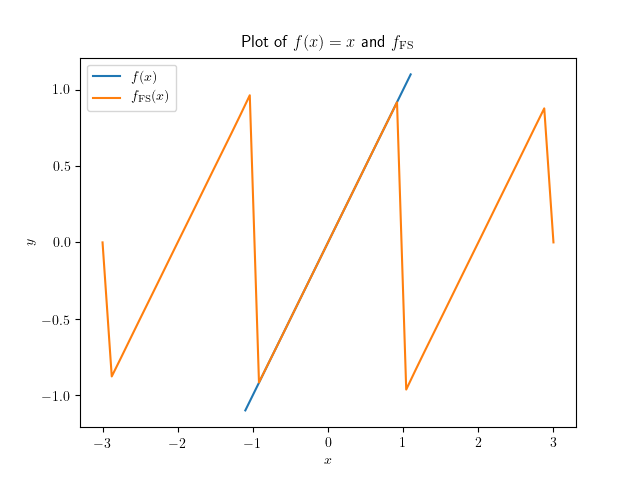
\includegraphics[scale=0.6]{fourier_series_x.png}
        \caption{A plot of \(f(x) = x\) and its Fourier series showing discontinuities.}
    \end{figure}
    
    Similarly if \(f(x) = x^2\) then as we can see from figure~\ref{fig:fourier series x^2} \(f_\FS\) is continuous but \(f_\FS'\) has discontinuities at \(L\).
    Therefore we expect
    \[a_n \sim \frac{1}{n^2}\]
    as \(p = 1\).
    \(b_n = 0\) since \(f\) is an even function.
    
    \subsection{Error}
    We define the error of the \(N\)th partial Fourier series to be
    \[D_N = \int_{-L}^{L} \dd{x}\abs{f(x) - f_{\FS, N}(x)}^2 = \lnorm[2]{f - f_{\FS,N}}^2.\]
    Here \(\lnorm[2]{\cdot}\) is the \(L^2\) norm defined on a function in \(\squareIntegrable(I)\) to be
    \[\lnorm[2]{f}^2 = \int_I \dd{x} \abs{f(x)}^2 = \innerproduct{f}{f}.\]
    As \(N\to\infty\) \(D_N\to 0\).
    
    \begin{example}
        The sign function, \(\sgn\), is defined as
        \[
            f(x) = \sgn(x) = 
            \begin{cases}
                +1, & x \ge 0,\\
                -1, & x < 0.
            \end{cases}
        \]
        We will find the Fourier series of \(\sgn\) over \([-1, 1]\).
        This function is odd and so \(a_n = 0\) for all \(n\).
        We can calculate the \(b_n\) components fairly easily:
        \begin{align*}
            b_n &= 2 \int_0^1 \dd{x} \sgn(x)\sin(n\pi x)\\
            &= 2 \int_0^1 \dd{x} \sin(n\pi x)\\
            &= 2\left[-\frac{1}{n\pi}\cos(n\pi x)\right]_0^1\\
            &= -\frac{2}{n\pi}[(-1)^n - 1]\\
            &= \frac{2}{n\pi}[1 - (-1)^n]
        \end{align*}
        This has been plotted in figure~\ref{fig:sgn fourier}.
    \end{example}
    \begin{figure}[ht]
        \centering
        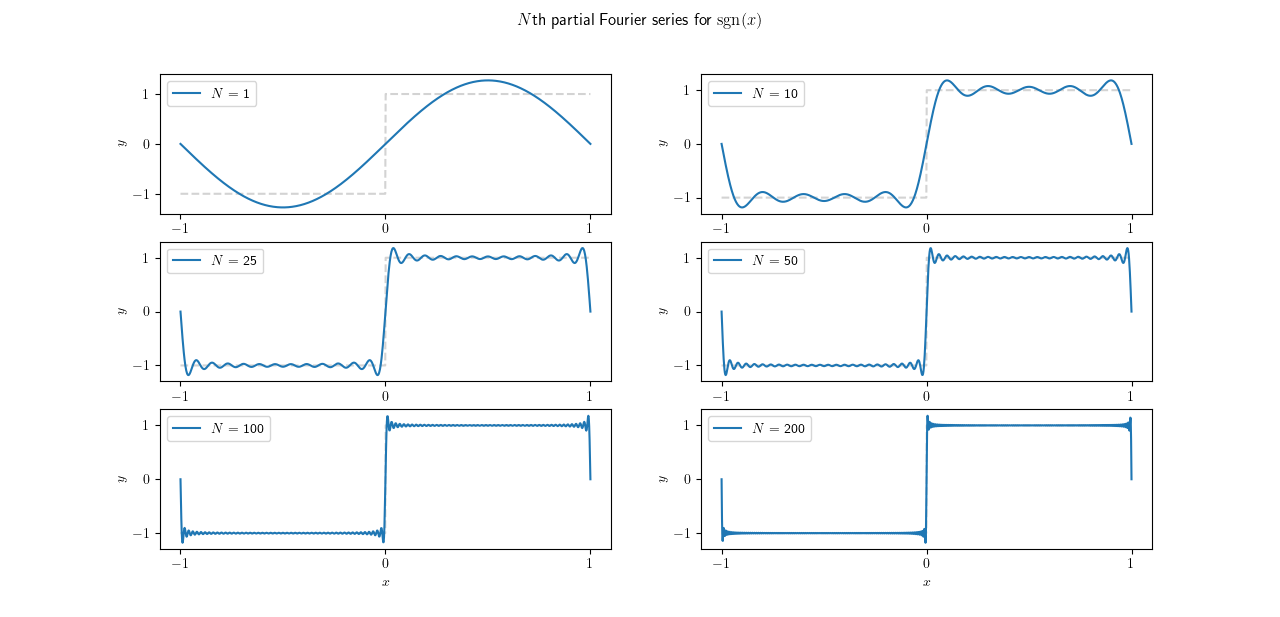
\includegraphics[scale=0.5]{sgn_fourier.png}
        \caption{\(N\)th partial Fourier series of \(\sgn\) plotted at various values of \(N\).}
        \label{fig:sgn fourier}
    \end{figure}
    \subsection{Gibbs' Phenomenon}
    Figure~\ref{fig:sgn fourier} shows the \(N\)th partial Fourier series of \(\sgn\) for various values of \(N\).
    Note how at the discontinuities, which in this case occur at all integers, the Fourier series has a large error compared to everywhere else.
    This is called \define{Gibbs phenomenon} and occurs whenever there is a discontinuity.
    Importantly adding terms doesn't completely get rid of it until we have an infinite number of terms.
    
    \subsection{Parseval's Theorem}
    \define{Parseval's theorem} states that if \(f\colon\reals\to\complex\) has a complex Fourier series with coefficients, \(c_n\), then
    \[\frac{1}{2L}\int_{-L}^{L} \dd{x}\abs{f(x)}^2 = \frac{1}{2L}\lnorm[2]{f}^2 = \sum_{n\in\integers}\abs{c_n}^2.\]
    If instead \(f\colon\reals\to\reals\) has a real Fourier series with coefficients, \(a_n\) and \(b_n\), then
    \[\frac{1}{2L}\int_{-L}^{L} \dd{x}\abs{f(x)}^2 = \frac{1}{2L}\lnorm[2]{f}^2 = \abs{\frac{a_0}{2}}^2 +  \sum_{n=1}^{\infty}[\abs{a_n}^2 + \abs{b_n}^2].\]
    
    Compare these statements with the statement that for \(\vv{v}\in\complex^n\)
    \[\norm{\vv{v}}^2 = \sum_{i=1}^{n} \abs{v_i}^2.\]
    The quantity \(\abs{c_n}^2\) is known as the power spectrum.
    This is in analogy with an electric circuit where the average power is proportional to \(\abs{I}^2\).
    We can view \(\lnorm[2]{f}^2\) as the average power and \(\abs{c_n}^2\) as the contribution of the \(n\)th mode.
    
    \begin{theorem}[Parseval's Theorem]
        If \(f\colon\reals\to\complex\) has a Fourier series,
        \[f_\FS(x) = \sum_{n\in\integers} c_n\varphi_n(x),\]
        then
        \[\frac{1}{2L}\lnorm[2]{f}^2 = \sum_{n\in\integers}\abs{c_n}^2.\]
    \end{theorem}
    \begin{proof}
        The \(L^2\) norm of \(f\) is defined to be
        \begin{align*}
            \frac{1}{2L}\lnorm[2]{f}^2 &= \frac{1}{2L}\int_{-L}^{L} \dd{x} f(x)f^*(x)
            \shortintertext{substituting in the Fourier series of \(f\) gives}
            &= \frac{1}{2L} \int_{-L}^{L} \dd{x} \left[\sum_{n\in\integers} c_n\varphi_n(x)\right] \left[\sum_{m\in\integers} c_m^*\varphi_m(x)\right]
            \shortintertext{Since the sums and integrals are over different variables they commute}
            &= \frac{1}{2L} \sum_{\mathclap{n, m\in\integers}} c_nc_m^* \int_{-L}^{L} \dd{x} \varphi_n(x)\varphi_m^*(x)
            \shortintertext{identifiying the integral as the inner product gives}
            &= \frac{1}{2L} \sum_{\mathclap{n, m\in\integers}} c_nc_m^* \innerproduct{\varphi_m}{\varphi_n}\\
            &= \frac{1}{2L} \sum_{\mathclap{n, m\in\integers}} c_nc_m^*2L\delta_{mn}\\
            &= \sum_{n, m\in\integers} c_nc_m^* \delta_{mn}\\
            &= \sum_{n\in\integers} c_nc_n^*\\
            &= \sum_{n\in\integers} \abs{c_n}^2.
        \end{align*}
    \end{proof}
    \begin{theorem}
        If \(f\colon\reals\to\reals\) has a Fourier series,
        \[f_\FS(x) = \frac{a_0}{2} + \sum_{n=1}^{\infty} [a_n\cos(k_nx) + b_n\sin(k_nx)],\]
        then
        \[\frac{1}{2L}\lnorm[2]{f}^2 = \sum_{n=1}^{\infty}\left[\abs{a_n}^2 + \abs{b_n}^2\right].\]
    \end{theorem}
    \begin{proof}
        From the previous theorem we know that
        \[\frac{1}{2L}\lnorm[2]{f}^2 = \sum_{n\in\integers}\abs{c_n}^2.\]
        We have also shown previously that
        \[c_n = \frac{1}{2}[a_n - ib_n],\qquad\text{and}\qquad c_n^* = \frac{1}{2}[a_n + ib_n].\]
        Combining these we have
        \begin{align*}
            \frac{1}{2L}\lnorm[2]{f}^2 &= \sum_{n\in\integers}\abs{c_n}^2\\
            &= \sum_{n\in\integers}c_nc_n^*\\
            &= \sum_{n\in\integers}\frac{1}{2}[a_n - ib_n]\frac{1}{2}[a_n + ib_n]\\
            &= \frac{1}{4}\sum_{n\in\integers}[a_n - ib_n][a_n + ib_n]
            \shortintertext{splitting the sum gives}
            &= \frac{1}{4}[a_0 - ib_0][a_0 + ib_0] + \frac{1}{4}\sum_{\mathclap{n\in\integers^+}}[a_n - ib_n][a_n + ib_n] + \frac{1}{4}\sum_{\mathclap{n\in\integers^-}}[a_n - ib_n][a_n + ib_n]
            \shortintertext{noting that \(b_0 = 0\) we hvae}
            &= \frac{1}{4}\abs{a_0}^2 + \frac{1}{4}\sum_{\mathclap{n\in\integers^+}}[a_n - ib_n][a_n + ib_n] + \frac{1}{4}\sum_{\mathclap{n\in\integers^-}}[a_n - ib_n][a_n + ib_n]
            \shortintertext{renaming the dummy index \(n\to-n\) in the last sum gives}
            &= \frac{1}{4}\abs{a_0}^2 + \frac{1}{4}\sum_{\mathclap{n\in\integers^+}} [a_n - ib_n][a_n + ib_n] + \frac{1}{4}\sum_{\mathclap{n\in\integers^+}} [a_{-n} - ib_{-n}][a_{-n} + ib_{-n}]
            \shortintertext{now using the fact that \(a_{-n} = a_n\) and \(b_{-n} = -b_n\) we get}
            &= \frac{1}{4}\abs{a_0}^2 + \frac{1}{4}\sum_{n=1}^{\infty}[a_n - ib_n][a_n + ib_n] + \frac{1}{4}\sum_{n=1}^{\infty}[a_n + ib_n][a_n - ib_n]
            \shortintertext{now noting that the two sums are the same}
            &= \frac{1}{4}\abs{a_0}^2 + \frac{1}{2}\sum_{n=1}^{\infty}[a_n - ib_n][a_n + ib_n]
            \shortintertext{finally expanding the brackets in the sum we get}
            &= \frac{1}{4}\abs{a_0}^2 + \frac{1}{2}\sum_{n=1}^{\infty}\left[\abs{a_n}^2 + \abs{b_n}^2\right]
        \end{align*}
    \end{proof}
    \subsubsection{Summing Series via Parseval}
    Let \(f(x) = x^2\).
    Find \(\lnorm[2]{f}^2/2L\).
    First we will calculate this explicitly:
    \begin{align*}
        \frac{1}{2L}\lnorm[2]{f}^2 &= \frac{1}{2L}\int_{-L}^{L} \dd{x} \abs{f(x)}^2\\
        &= \frac{1}{2L}\int_{-L}^{L} \dd{x} x^4\\
        &= \frac{1}{2L}\left[\frac{1}{5}x^5\right]_{-L}^{L}\\
        &= \frac{1}{5}L^4.
    \end{align*}
    We can also calculate this value using Parseval's theorem.
    We previously calculated that for \(f(x) = x^2\)
    \[
        c_n = 
        \begin{cases}
            \frac{L^2}{3}, & n = 0,\\
            \frac{2L^2}{n^2\pi^2}(-1)^n, & n \ne 0.
        \end{cases}
    \]
    Thus
    \begin{align*}
        \frac{1}{2L}\lnorm[2]{f}^2 &= \sum_{n\in\integers}\abs{c_n}^2\\
        &= \abs{c_0}^2 + \sum_{\mathclap{n\in\integers\setminus\{0\}}}\abs{c_n}^2\\
        &= \left(\frac{L^2}{3}\right)^2 + \sum_{n\in\integers\setminus\{0\}} \left(\frac{2L^2(-1)^n}{n^2\pi^2}\right)^2
        \shortintertext{noting that each term of the sum is equal for \(n\) and \(-n\) the sum becomes}
        &= \frac{L^4}{9} + 2\sum_{n=1}^{\infty} \frac{4L^4}{n^4\pi^4}\\
        &= \frac{L^4}{9} + \frac{8L^4}{\pi^4}\sum_{n=1}^{\infty} \frac{1}{n^4}.
    \end{align*}
    Equating this to the result from the explicit calculation and rearranging we get
    \[\frac{\pi^4}{90} = \sum_{n=1}^{\infty}\frac{1}{n^4} = \zeta(4).\]
    This gives us a new approximation of \(\pi\) that converges even quicker than our previous approximations:
    \[\hat{\pi}_N = \left(90\sum_{n=1}^{N}\frac{1}{n^4}\right)^{1/4}.\]
    Some evaluations of this are given in table~\ref{tab:pi_N 3}
    \begin{table}[ht]
        \centering
        \begin{tabular}{rcc}\hline
            \(N\) & \(\hat{\pi}_N\) & \(\hat{\pi}_N - \pi\)\\\hline
            1 & 3.0800702882 & -0.0615223653\\
            2 & 3.1271078664 & -0.0144847872\\
            3 & 3.1361523798 & -0.0054402738\\
            4 & 3.1389978894 & -0.0025947642\\
            5 & 3.1401611795 & -0.0014314741\\
            6 & 3.1407217179 & -0.0008709357\\
            7 & 3.1410241579 & -0.0005684956\\
            8 & 3.1412014021 & -0.0003912515\\
            9 & 3.1413120396 & -0.0002806140\\
            10 & 3.1413846225 & -0.0002080311\\
            100 & 3.1415924153 & -0.0000002383\\
            1000 & 3.1415926533 & -0.0000000002\\
            10000 & 3.1415926536 & -0.0000000000\\\hline
        \end{tabular}
        \caption{\(\hat{\pi}_N\) evaluated at various values of \(N\).}
        \label{tab:pi_N 3}
    \end{table}

    \section{Fourier Transforms}
    The indicator function, \(1_A\colon X\to \{0, 1\}\), is a function defined by
    \[
        1_A(x) = 
        \begin{cases}
            1, & x\in A,\\
            0, & x\notin A.
        \end{cases}
    \]
    That is \(1_A(x)\) is one if and only if \(x\in A\).
    One use of this function is to define a pulse, \(1_{[-a, a]}\), which is non-zero only for \(x\in[-a, a]\).
    The Fourier series, extended to all real numbers, of \(1_{[-a, a]}\) is shown in figure~\ref{fig:indicator} with increasing values of \(L\) chosen.
    \begin{figure}[ht]
        \centering
        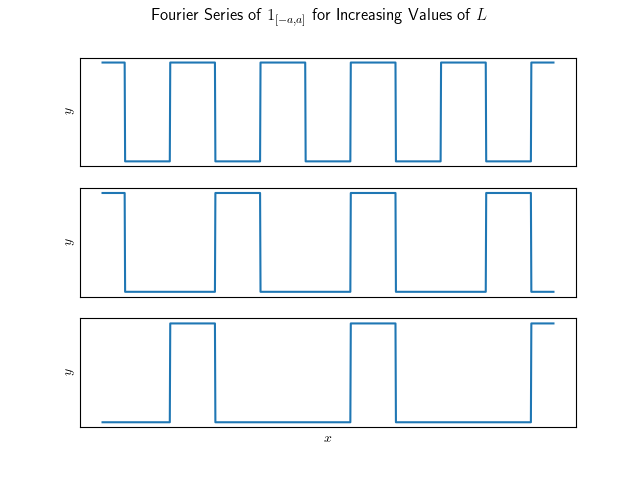
\includegraphics[scale=0.6]{indicator_ft.png}
        \caption{The Fourier series of the indicator function, \(1_{[-a, a]}\) for various values of \(L\) with \(L\) increasing down the plots.}
        \label{fig:indicator}
    \end{figure}
    It is clear that in the limit of \(L\to\infty\) the Fourier series will exactly match the original function everywhere.
    This is the idea between the Fourier transform.
    
    \subsection{Deriving The Fourier Transform}
    A Fourier series exactly describes a function, \(f\colon\reals\to\complex\), for \(x\in[-L, L]\).
    If we take the limit as \(L\to\infty\) then we get an exact description of \(f\) for \(x\in(-\infty, \infty) = \reals\).
    If \(f\colon\reals\to\complex\) then we can expand this as a Fourier series
    \[f_\FS(x) = \sum_{n\in\integers} c_ne^{ik_nx}.\]
    The coefficients are calculated as
    \[c_n = \frac{1}{2L}\int_{-L}^{L} \dd{x} f(x) e^{-in\pi x/L} = \frac{1}{\ell}\int_{-\ell/2}^{\ell/2}\dd{x} f(x)e^{-2in\pi x/\ell} = \frac{1}{\ell}\int_{-\ell/2}^{\ell/2}\dd{x}f(x)e^{-ik_nx}.\]
    Here we have defined \(\ell = 2L\) to be the fundamental period of the Fourier series extended to \(\reals\).
    Currently \(c_n\) and \(k_n\) are discrete variables.
    In the following limit they will become continuous.
    In particular \(k_n\to k\) and \(c_n \to c(k)\) where
    \[c(k) = \lim_{\ell\to\infty} c_n = \lim_{\ell\to\infty} \frac{1}{\ell}\int_{-\ell/2}^{\ell/2}\dd{x} f(x)e^{-ik_nx}.\]
    Further we define
    \[\FT[f](k) = \tilde{f}(k) = \lim_{\ell\to\infty} \ell c(k) = \int_{-\infty}^{\infty} \dd{x} f(x) e^{-ikx}.\]
    \(\FT[f] = \tilde{f}\) is the \define{Fourier transform} of \(f\).
    
    \subsection{The Inverse Fourier Transform}
    Further we can calculate the \define{inverse Fourier transform} which allows us to recover \(f\) from \(\tilde{f}\).
    For this we will need the value
    \[\Delta k = k_{n+1} - k_n = \frac{2\pi}{\ell}.\]
    Expanding \(f\) as a Fourier series with \(\ell\to\infty\) we have
    \begin{align*}
        f(x) &= \lim_{\ell\to\infty} \sum_{n\in\integers} c_n e^{ik_nx}\\
        &= \lim_{\ell\to\infty} \sum_{n\in\integers} \frac{\Delta k}{\frac{2\pi}{\ell}} c_n e^{-ik_nx}\\
        &= \frac{1}{2\pi}\lim_{\ell\to\infty} \sum_{n\in\integers}\Delta k\ell c_n e^{ik_nx}
        \shortintertext{noting that in the limit \(\ell c_n\to \tilde{f}(k)\) we have}
        &= \frac{1}{2\pi}\int_{-\infty}^{\infty} \dd{k} \tilde{f}(k)e^{ikx}.
    \end{align*}
    The set of possible values of \(k\) is called \(k\)-space, Fourier space, momentum space, or frequency space.
    The first two are general and the second two are for the common cases where the units of \(k\) are units momentum or inverse time respectively.
    Similarly the set of possible values of \(x\) is called \(x\)-space, real space, coordinate space, position space, or time space.
    Again the first three are general, coordinate and position space both refer to when \(x\) has units of distance and time space refers to when \(x\) has units of time.
    
    We can transform between real space and Fourier space easily with a Fourier transform and inverse Fourier transform:
    \[\FT[f](k) = \tilde{f}(k) = \int_{-\infty}^{\infty} \dd{x} f(x) e^{-ikx},\qquad\text{and}\qquad \FT^{-1}[\tilde{f}](x) = f(x) = \frac{1}{2\pi}\int_{-\infty}^{\infty} \dd{k} \tilde{f}(k)e^{ikx}.\]
    Note that there are a few conventions here.
    Some texts place the factor of \(2\pi\) in the forward Fourier transform, others include a factor of \(\sqrt{2\pi}\) in both the forward and inverse Fourier transform.
    Which exponent has a negative is also convention.
    Finally sometimes a factor of \(2\pi\) will be included in the exponents.
    
    \subsection{Properties of the Fourier Transform}
    The Fourier transform is linear, that is for \(f, g\colon\reals \to \complex\) and \(a, b\in\complex\)
    \[\FT[af + bg] = a\FT[f] + b\FT[g].\]
    
    The Fourier transform of \(f\colon\reals\to\reals\) is \define{hermitian} in that
    \[\tilde{f}(k) = \tilde{f}^*(-k).\]
    This is fairly easy to show.
    Since \(f(x)\in\reals\A x\in\reals\) \(f = f^*\).
    Computing the complex conjugate of \(f\) is as simple as taking the complex conjugate of the inverse Fourier transform of \(\tilde{f}\):
    \begin{align*}
        f^*(x) &= \left[\frac{1}{2\pi}\int_{-\infty}^{\infty} \dd{k} \tilde{f}(k) e^{ikx}\right]^*\\
        &= \frac{1}{2\pi} \int_{-\infty}^{\infty} \dd{k} \tilde{f}^*(k)e^{-ikx}
        \shortintertext{Let \(k\to-k\), \(\dd{k}\to-\dd{k}\), \((-\infty, \infty)\to(\infty, -\infty)\):}
        &= -\frac{1}{2\pi} \int_{\infty}^{-\infty} \dd{k} \tilde{f}^*(-k) e^{ikx}\\
        &= \frac{1}{2\pi} \int_{-\infty}^{\infty} \dd{k} \tilde{f}^*(-k) e^{ikx}.
    \end{align*}
    Now since \(f = f^*\) we must have that this is equal to
    \[f(x) = \frac{1}{2\pi}\int_{-\infty}^{\infty} \tilde{f}(k)e^{ikx}.\]
    Noting that both integrals have the same limits and that \(e^{ikx}\ne 0\) we must have
    \[\tilde{f}(k) = \tilde{f}^*(-k).\]
    
    
    \section{Reciprocal Relation}
    The reciprocal relation between a function and its Fourier transform is that if there is some measure of width of the functions then the width of the function is inversely proportional to the width of the Fourier transform.
    This turns out to be important in several areas:
    \begin{itemize}
        \item The Heisenberg uncertainty principle -- The uncertainty in position, \(\Delta x\), and uncertainty in momentum, \(\Delta p\), are inversely related:
        \[\Delta x\Delta p \ge \frac{\hbar}{2}.\]
        \item The bandwidth theorem -- To create a short pulse of length \(\Delta t\) a large range of frequencies, \(\Delta\omega\), is needed.
        \item Optics -- The narrower a slit the wider the diffraction pattern.
    \end{itemize}
    We will look at two functions with easily defined widths and how they relate to physics.
    
    \subsection{Fourier Transform of the Top Hat Function}
    The top hat function, \(\Pi_a(x)\) is defined as
    \[
        \Pi_a(x) =
        \begin{cases}
            h, & x\in[d - a, d + a],\\
            0, & x\notin[d - a, d + a].
        \end{cases}
    \]
    First note that
    \[\int_{-\infty}^{\infty} \dd{x} \Pi_a(x) = h\int_{d-a}^{d+a} \dd{x}.\]
    The Fourier transform can then be calculated:
    \begin{align*}
        \tilde{\Pi}_a(k) &= \int_{-\infty}^{\infty} \dd{x} \Pi_a(x)e^{-ikx}\\
        &= h\int_{d-a}^{d+a} \dd{x} e^{-ikx}\\
        &= h\left[-\frac{1}{ik}e^{-ikx}\right]_{d-a}^{d+a}\\
        &= \frac{ih}{k}\left[e^{-ik(d-a)} - e^{-ik(d+a)}\right]\\
        &= \frac{ih}{k}e^{-ikd}\left[e^{ika} - e^{-ika}\right]\\
        &= \frac{ih}{k}e^{-ikd}\left[-2i\sin(ka)\right]\\
        &= \frac{2h}{k}e^{-ikd}\sin(ka)\\
        &= 2ahe^{-ikd}\frac{\sin(ka)}{ka}\\
        &= 2ahe^{-ikd}\sinc(ka)
    \end{align*}
    Here we have introduced the \(\sinc\) function defined as
    \[\sinc(x) = \frac{\sin(x)}{x}.\]
    This is of an indeterminate form at \(x = 0\).
    We can apply L'H\^opital's rule:
    \[\lim_{x\to 0}\sinc(x) = \lim_{x\to 0}\frac{\sin(x)}{x} = \lim_{x\to 0}\frac{\dv{x}\sin(x)}{\dv{x}x} = \lim_{x\to 0}\frac{\cos(x)}{1} = 1.\]
    The \(\sinc\) function is plotted in figure~\ref{fig:sinc}.
    \begin{figure}[ht]
        \centering
        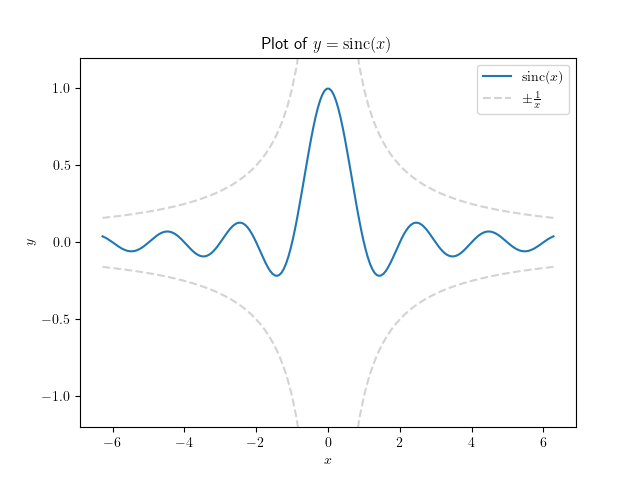
\includegraphics[scale=0.6]{sinc.png}
        \caption{The \(\sinc\) function}
        \label{fig:sinc}
    \end{figure}
    The nodes of \(\sinc(ka)\), where \(\sinc(ka) = 0\), occur at \(ka = n\pi\) for \(n\in\integers\setminus\{0\}\).
    This means that the distance between nodes is
    \[k = \frac{n\pi}{a}.\]
    This is inversely proportional to \(a\), which is half the width of the top hat function.
    
    This relationship is important in optics.
    A slit can be modelled as a top hat function, light is emitted only between \(d-a\) and \(d+a\).
    The interference pattern that is then projected onto a screen is given by the square of the absolute value of the Fourier transform of this slit, which means it is proportional to \(\abs{\sinc(ka)}^2\).
    The narrower the slit the further apart the nodes of the interference pattern will be.
    
    \subsection{Fourier Transform of a Gaussian}\label{sec:Fourier transform of a Gaussian}
    A Gaussian, with mean \(\mu = 0\), is defined by
    \[f(x) = e^{-\frac{x^2}{2\sigma^2}}.\]
    It is known that
    \[\int_{-\infty}^{\infty} \dd{x} f(x) = \sqrt{2\pi\sigma^2}.\]
    This holds for a Gaussian with any mean.
    Here \(\sigma\) is the standard deviation and provides a measure of the width of the Gaussian.
    The Fourier transform can be computed with relative ease:
    \begin{align*}
        \tilde{f}(k) &= \int_{-\infty}^{\infty} \dd{x}f(x)e^{-ikx}\\
        &= \int_{-\infty}^{\infty} \dd{x} e^{-\frac{x^2}{2\sigma^2}} e^{-ikx}\\
        &= \int_{-\infty}^{\infty} \dd{x} e^{-\frac{x^2}{2\sigma^2}-ikx}\\
        &= \int_{-\infty}^{\infty} \dd{x} e^{-\frac{1}{2\sigma^2}[x^2 + 2i\sigma^2kx]}
        \shortintertext{Completeing the square in the exponent, we use that \((x + a/2)^2 = x^2 + ax + a^2/4\) so \(x^2 + ax = (x + a/2)^2 - a^2/4\):}
        &= \int_{-\infty}^{\infty} \dd{x} e^{-\frac{1}{2\sigma^2}\left[(x + ik\sigma^2) - \frac{1}{4}(ik2\sigma^2)^2\right]}\\
        &= \int_{-\infty}^{\infty} \dd{x} e^{-\frac{1}{2\sigma^2}(x + ik\sigma^2) - \frac{k^2\sigma^2}{2}}\\
        &= e^{-\frac{k^2\sigma^2}{2}} \int_{-\infty}^{\infty} \dd{x} e^{-\frac{1}{2\sigma^2}(x + ik\sigma^2)^2}
        \shortintertext{Note that the integrand is now a Gaussian with mean \(ik\sigma^2\), so the integral is simply \(\sqrt{2\pi\sigma^2}\), that this holds for complex means is beyond the scope of this course to show.}
        &= e^{-\frac{k^2\sigma^2}{2}}\sqrt{2\pi\sigma^2}.
    \end{align*}
    This is simply another Gaussian with standard deviation \(\tilde{\sigma} = 1/\sigma\).
    
    \subsubsection{Heisenberg's Uncertainty Principle}
    Suppose that \(x\) represents the position of a particle.
    In quantum mechanics the best we can do is get a probability distribution for this observable.
    The central limit theorem allows us to approximate this as a Gaussian.
    The wave function of a particle is such that its square gives the probability density function.
    Consider the wave function
    \[\psi(x) = e^{-\frac{x^2}{2\sigma^2}}\]
    The associated probability density function is
    \[\abs{\psi(x)}^2 = e^{-\frac{x^2}{\sigma^2}}.\]
    This has a width of
    \[\Delta x = \frac{\sigma}{\sqrt{2}}.\]
    
    De Broglie noticed that the momentum, \(p\), and wave number, \(k\), of a particle were related by
    \[p = \hbar k.\]
    \(k\) here is exactly the same as the \(k\) we have been using for a Fourier transform variable.
    The Fourier transformed wave function is thus
    \[\tilde{\psi}(k) = \sqrt{2\pi\sigma^2}e^{-\frac{k^2\sigma^2}{2}}.\]
    This is more commonly written in terms of the momentum:
    \[\tilde{\psi}(p) = \sqrt{2\pi\sigma^2} e^{-\frac{p^2\sigma^2}{2\hbar^2}}.\]
    The associated probability density function is then
    \[\abs{\tilde{\psi}(p)}^2 = 2\pi\sigma^2e^{-\frac{p^2\sigma^2}{\hbar^2}}.\]
    This has a width of
    \[\Delta p = \frac{\hbar}{\sigma\sqrt{2}}.\]
    From this it follows that
    \[\Delta x\Delta p = \frac{\sigma}{\sqrt{2}} \frac{\hbar}{\sigma\sqrt{2}} = \frac{\hbar}{2}.\]
    It can be shown that for any initial wave function that is not a Gaussian then \(\Delta x\Delta p\) will be larger than this.
    Similarly it can be shown that if energy is quantised and \(E = \hbar\omega\), where \(\omega\) plays the role of the Fourier transformed variable then
    \[\Delta E\Delta t \le \frac{\hbar}{2}.\]
    
    \section{The Dirac Delta Distribution}
    In section~\ref{sec:dirac delta} we introduced the Dirac delta distribution, defined by
    \[
        \delta(x - d) =
        \begin{cases}
            1, & x = d,\\
            0, & x\ne d,
        \end{cases}
    \]
    and
    \[\int_{-\infty}^{\infty} \dd{x}\delta(x - d) = 1.\]
    Here we will look at this distribution in more detail.
    
    \subsection{Dirac Delta of a function}
    Suppose \(f\colon S\to\reals\).
    What is \(\delta(f(x))\)?
    Starting from the normalisation condition we have
    \[\int_S \dd{f}\delta(f) = 1.\]
    Performing a change of variables with the Jacobian this becomes
    \[\int_{-\infty}^{\infty} \dd{x}\abs{\dv{f}{x}}\delta(f(x)) = 1.\]
    We know that \(\delta(f(x)) = 0\) whenever \(f(x) = 0\).
    Denote by \(x_i\) the zeros of \(f\) such that \(f(x_i) = 0\).
    We can split the integral into small regions around each pole:
    \[\sum_i \int_{x_i - \varepsilon}^{x_i + \varepsilon} \dd{x} \abs{\dv{f}{x}}\delta(f(x)) = 1.\]
    Here \(\varepsilon > 0\) is some number small enough that \(x_i\) is the only zero of \(f\) that falls in the interval \([x_i - \varepsilon, x_i + \varepsilon]\).
    The only important property of the argument of the delta distribution is when it is zero.
    Therefore over the interval \([x_i - \varepsilon, x_i + \varepsilon]\) \(\delta(f(x)) = A\delta(x - x_i)\) where \(A\) is a normalisation constant.
    Thus we have
    \[A\sum_i \int_{x_i - \varepsilon}^{x_i + \varepsilon} \dd{x} \abs{\dv{f}{x}}\delta(x - x_i) = 1.\]
    Applying the sifting property of the delta distribution, noting that \(\abs{\inlinedv{f}{x}}\) is simply a function of \(x\), we have
    \[A\sum_i\abs{\dvat{f}{x}{x_i}} = 1.\]
    Hence
    \[A = \sum_i \frac{1}{\abs{f'(x_i)}}.\]
    So we conclude that
    \[\delta(f(x)) = \sum_i \frac{\delta(x - x_i)}{\abs{f'(x_i)}}.\]
    
    A few specific cases of this are worth considering:
    \begin{itemize}
        \item \(f(x) = -x\), then \(f'(x) = -1\) and \(\abs{f'(x)} = 1\) so \(\delta(-x) = \delta(f(x)) = \delta(x)/1 = \delta(x)\).
        \item \(f(x) = ax\), then \(f'(x) = a\) and \(\abs{f'(x)} = \abs{a}\) so \(\delta(ax) = \delta(f(x)) = \delta(x)/\abs{a}\).
        \item \(f(x) = x^2 - a^2\), then \(f'(x) = 2x\), \(f\) has two roots, \(\pm a\), so
        \[\delta(x^2 - a^2) = \delta(f(x)) = \frac{\delta(x - a)}{2\abs{a}} + \frac{\delta(x + a)}{2\abs{a}}.\]
    \end{itemize}

    \subsection{Sifting Property Revisited}
    Previously in section~\ref{sec:sifting property dirac delta} we showed the sifting property of the Dirac delta distribution taking the delta distribution as a limit of a top hat function.
    This requires \(f\) be continuous at which ever point the delta distribution is non-zero.
    Here we will use an alternative method that assumes \(f\) is infinitely differentiable at that point.
    If this is the case then we can again view \(\delta(x)\) as a limit of a top hat function and expand \(f\) as a Taylor series:
    \begin{align*}
        \int_{-\infty}^{\infty} \dd{x} f(x)\delta(x) &= \lim_{a\to 0} \int_{-\infty}^{\infty} \dd{x} f(x)\Pi_a(x)\\
        &= \lim_{a\to 0} \frac{1}{2a} \int_{-a}^{a} \dd{x} f(x)\\
        &= \lim_{a\to 0} \frac{1}{2a} \int_{-a}^{a} \dd{x}\left[f(0) + f'(0)x + \frac{1}{2}f''(0)x^2 + \order{x^3}\right]\\
        &= \lim_{a\to 0} \frac{1}{2a} \left[f(0)x + f'(0)x^2 + \frac{1}{6}f''(0)x^3 + \order{x^4}\right]_{-a}^{a}\\
        &= \lim_{a\to 0} \frac{1}{2a} \left[f(0)(a - (-a)) + f'(0)(a^2 - (-a)^2) + \frac{1}{6}f''(0)(a^3 - (-a)^3) + \order{a^4}\right]\\
        &= \lim_{a\to 0} \frac{1}{2a} \left[2af(0) + \frac{a^3}{3}f''(0) + \order{a^5}\right]\\
        &= \lim_{a\to 0} \left[f(0) + \frac{a^2}{6}f''(0) + \order{a^4}\right]\\
        &= f(0).
    \end{align*}
    Here we have used that \(f^{(n)}(0)\) is simply a constant.
    
    \subsection{Calculus with Delta Distributions}
    \subsubsection{Integral of the Delta Distribution}
    The normalisation condition can be restated as
    \[
        \int_a^b \dd{x} \delta(x - d) = 
        \begin{cases}
            1, & d\in[a, b],\\
            0, & d\notin[a, b].
        \end{cases}
    \]
    In particular
    \[
        \int_{-\infty}^{x} \dd{y} \delta(y - d) =
        \begin{cases}
            1, & x \ge d\\
            0, & x < d
        \end{cases}
        = \Theta(x - d)
    \]
    This is exactly the definition of the \define{Heaviside step function}:
    \[
        \Theta(x) =
        \begin{cases}
            1, & x \ge 0,\\
            0, & x < 0.
        \end{cases}
    \]
    By the fundamental theorem of calculus we must also then have that
    \[\dv{x}\Theta(x) = \delta(x).\]
    
    \subsubsection{Derivative of the Delta Distribution}
    By the sifting property we must have that
    \[f(x)\delta(x) = f(0)\delta(x).\]
    Differentiating we get
    \[\dv{x}[f(x)\delta(x)] = f'(x)\delta(x) + f(x)\delta'(x).\]
    Rearranging we get
    \[f(x)\delta'(x) = \dv{x}[f(x)\delta(x)] - f'(x)\delta(x)\]
    Integrating over this we have
    \begin{align*}
        \int_{-\infty}^{\infty} \dd{x} f(x)\delta'(x) &= \int_{-\infty}^{\infty} \dd{x}\dv{x}[f(x)\delta(x)] - \int_{-\infty}^{\infty} \dd{x} f'(x)\delta(x)\\
        &= [f(x)\delta(x)]_{-\infty}^{\infty} - \int_{-\infty}^{\infty} \dd{x}f'(x)\delta(x)\\
        &= -f'(0)
    \end{align*}
    since \(\delta\) vanishes at infinity so the first term is zero.
    The sifting property can then be applied to the second term.
    Since the integrals are over the same interval the integrands must be equal:
    \[f(x)\delta'(x) = -f'(0).\]
    
    \subsection{Delta Distributions in More Dimensions}
    If \(\vv{r}, \vv{r_0}\in\reals^n\) then
    \[\delta(\vv{r} - \vv{r_0}) = \prod_{i=1}^{n}\delta(x - x_i).\]
    In the case of \(n = 3\) with Cartesian coordinates we have
    \[\delta(\vv{r} - \vv{r_0}) = \delta(x - x_0)\delta(y - y_0)\delta(z - z_0).\]
    Be careful, \(\delta(\vv{r} - \vv{r_0})\ne \delta(r - r_0)\).
    The first picks out a point at \(\vv{r_0}\) the second picks out an annulus of radius \(r_0\).
    This is best shown for a spherically symmetric function, \(f\).
    This means that \(f(\vv{r}) = f(r)\).
    \[\int\dd{V}f(\vv{r})\delta(\vv{r} - \vv{r_0}) = f(\vv{r_0}) = f(r_0).\]
    \begin{align*}
        \int\dd{V}f(\vv{r})\delta(r - r_0) &= \int_0^{2\pi}\dd{\varphi}\int_0^{\pi}\sin\vartheta\dd{\vartheta} \int_0^{\infty} \dd{r}r^2f(\vv{r})\delta(r - r_0)\\
        &= 4\pi r_0^2f(r_0).
    \end{align*}

    \subsection{Physical Importance of the Delta Distribution}
    Suppose we have a collection of point particles of mass, \(m_i\), charge, \(q_i\), and at positions \(\vv{r_i}\), then the mass density, \(\rho_m\), and charge density, \(\rho_q\), are given by
    \begin{align*}
        \rho_m(\vv{r}) &= \sum_i m_i\delta(\vv{r} - \vv{r_i})\\
        \rho_q(\vv{r}) &= \sum_i q_i\delta(\vv{r} - \vv{r_i})
    \end{align*}
    Clearly given the prevalence of point particles in physics the Delta distribution is very important.
    
    \subsection{Units of the Delta Distribution}
    The normalisation condition,
    \[\int_{-\infty}^{\infty} \dd{x} \delta(x) = 1,\]
    allows us to assign units to \(\delta(x)\).
    Clearly 1 is dimensionless so \(\delta(x)\) must have units of inverse units of \(x\).
    In the case that \(x\) is a position \([x] = L\) so \([\delta(x)] = L^{-1}\).
    In the three dimensional case we have
    \[\int_V \dd{V}\delta(\vv{r}) = 1\]
    and so if \([V] = L^3\) then \([\delta(\vv{r})] = L^{-3}\).
    Importantly this gives the correct units to the densities in the previous section.
    
    \subsection{Fourier Transform of the Delta Distribution}
    Let \(f(x) = \delta(x - d)\).
    The Fourier transform of this is
    \begin{align*}
        \tilde{f}(k) &= \int_{-\infty}^{\infty} \dd{x} f(x)e^{-ikx}\\
        &= \int_{-\infty}^{\infty} \dd{x} \delta(x - d)e^{-ikx}\\
        &= e^{-ikd}.
    \end{align*}
    In the special case that \(d = 0\) we have \(\tilde{f}(k) = 1\).
    Notice that \(\delta(x)\) is infinitesimally narrow and \(1\) is infinitely wide, this agrees with the reciprocal relation.
    
    We can also calculate the inverse Fourier transform of the delta distribution:
    \begin{align*}
        \delta(x - d) &= \frac{1}{2\pi} \int_{-\infty}^{\infty} \dd{k} \tilde{f}(k)e^{ikx}\\
        &= \frac{1}{2\pi} \int_{-\infty}^{\infty} \dd{k} e^{-ikd}e^{ikx}\\
        &= \frac{1}{2\pi} \int_{-\infty}^{\infty} \dd{k} e^{ik(x - d)}.
    \end{align*}
    That this converges can be shown by considering \(\delta\) as a limiting case of a function with a more well defined integral, such as a Gaussian.
    This is called the \define{integral representation of the delta distribution}.
    
    Suppose we have a signal composed of oscillations all at a single frequency with wave number \(K\).
    Then the frequency distribution is
    \[\delta(k - K) = \frac{1}{2\pi}\int_{-\infty}^{\infty} \dd{x} e^{ix(k - K)}.\]
    Here we have used that if we are in \(k\)-space then we can view \(x\)-space as Fourier space.
    The delta distribution in \(k\)-space is defined the same as in \(x\)-space and has all the expected properties.
    
    \section{Convolutions}
    Let \(f\colon\reals\to\complex\) and \(g\colon\reals\to\complex\) the convolution of \(f\) and \(g\) is a a third function, \(f\convolution g\colon\reals\to\complex\) defined by
    \[(f\convolution g)(x) = \int_{-\infty}^{\infty} \dd{x'}f(x')g(x - x').\]
    We can think of \(f\) as a theoretical prediction and \(g\) as some blurring function.
    Then \(f\convolution g\) is the measurement that we get trying to measure \(f\).
    
    \begin{example}
        Let \(f(x) = \delta(x)\), this is like a case where our theory predicts a measurement exactly at \(x = 0\).
        Most errors follow a Gaussian so we choose \(g(x) = N_\sigma(x)\) sa our blurring function.
        Then when trying to make a measurement we get
        \[(\delta\convolution N_\sigma)(x) = \int_{-\infty}^{\infty} \dd{x'}\delta(x')N_\sigma(x - x') = N_\sigma(x).\]
        Therefore we expect that over multiple measurements we will get a Gaussian.
    \end{example}
    
    Convolution is a commutative operation.
    This is fairly easy to see.
    \[(f\convolution g)(x) = \int_{-\infty}^{\infty} \dd{x'}f(x') g(x - x').\]
    Let \(u = x - x'\) then \(\dd{u} = -\dd{x'}\) and \((-\infty, \infty)\rightarrow (\infty, -\infty)\):
    \begin{align*}
        (f\convolution g)(x) &= -\int_{\infty}^{-\infty} \dd{u}f(x - u) g(u)\\
        &= \int_{-\infty}^{\infty} \dd{u}g(u)f(x - u)\\
        &= (g \convolution f)(x).
    \end{align*}
    This holds for all \(x\) so
    \[f\convolution g = g\convolution f.\]
    
    \begin{example}
        Suppose we have a top-hat function
        \[
            \Pi_a(x) =
            \begin{cases}
                1/2a, & x \in [-a, a],\\
                0, & x\notin[-a, a].
            \end{cases}
        \]
        We can approximate the convolution of this with itself by computing the convolution at a few key points and guessing in between.
        The first key point is \(x = 0\):
        \begin{align*}
            (\Pi_a\convolution \Pi_a)(0) &= \int_{-\infty}^{\infty} \dd{x'} \Pi_a(x')\Pi_a(0 - x')\\
            &= \int_{-\infty}^{\infty} \dd{x'} \Pi_a(x')\Pi_a(x')\\
            &= \frac{1}{4a^2}\int_{-a}^{a} \dd{x'}\\
            &= \frac{1}{2a}.
        \end{align*}
        Here we have used that the top hat is symmetric and later that it is zero outside of \([-a, a]\).
        
        The next key point that we choose is \(x = a\):
        \begin{align*}
            (\Pi_a\convolution \Pi_a)(a) &= \int_{-\infty}^{\infty} \dd{x'} \Pi_a(x')\Pi_a(a - x')\\
            &= \frac{1}{4a^2}\int_{0}^{a}\dd{x'}\\
            &= \frac{1}{4a}.
        \end{align*}
        Here we have used that \(\Pi_a(x')\) is zero for all \(x'\notin[-a, a]\) and \(\Pi_a(a - x')\) is zero for all \(x'\notin[0, 2a]\).
        Therefore \(\Pi_a(x')\Pi_a(a - x')\) is zero for all \(x'\notin[-a, a]\intersection[0, 2a] = [0, a]\).
        On the other hand for \(x'\in[0, a]\) then \(\Pi_a(x')\Pi_a(a - x') = 1/4a^2\).
        
        The final key point is \(x = 2a\):
        \begin{align*}
            (\Pi_a\convolution \Pi_a)(2a) &= \int_{-\infty}^{\infty} \dd{x'} \Pi_a(x')\Pi_a(2a - x')\\
            &= \frac{1}{4a^2}\int_{a}^{a}\dd{x'}\\
            &= 0.
        \end{align*}
        Here we have used that \(\Pi_a(x')\) is zero for all \(x'\notin[-a, a]\) and \(\Pi_a(2a - x')\) is zero for all \(x'\notin[a, 3a]\) hence \(\Pi_a(x')\Pi_a(2a - x')\) is zero for all \(x'\notin[-a, a]\intersection[a, 3a] = \{a\}\), however an integral over a singleton is zero.
        
        Combining these and using the fact that a top hat is a union of horizontal lines we predict that the convolution of two top hats is a triangle function, \(\Delta_{2a}\), which is a triangle of base length \(4a\) centred on 0 with a peak height \(2a\).
        This is shown in figure~\ref{fig:triangle function}
        \begin{figure}[ht]
            \centering
            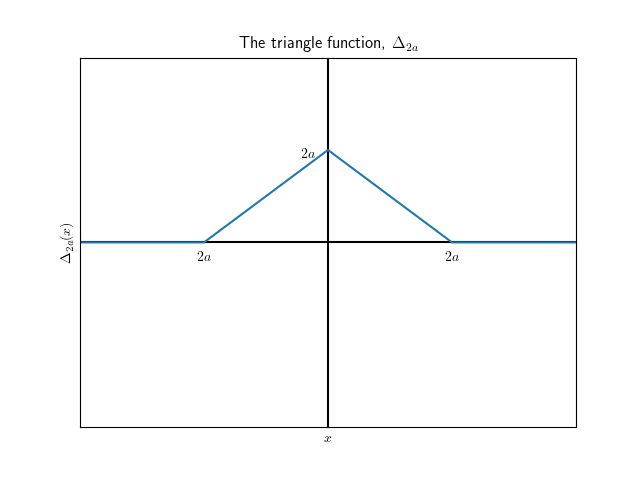
\includegraphics[scale=0.6]{triangle_function.png}
            \caption{The triangle function, \(\Delta_{2a}\), which is the convolution of two top hats, \(\Pi_a\convolution\Pi_a = \Delta_{2a}\).}
            \label{fig:triangle function}
        \end{figure}
    \end{example}
    
    \subsection{The Convolution Theorem}
    \begin{theorem}[Convolution Theorem]
        Let \(f, g\colon\reals\to\complex\).
        Then if \(\tilde{f}\) and \(\tilde{g}\) are the Fourier transforms of \(f\) and \(g\) we have
        \[\FT[f\convolution g](k) = \tilde{f}(k)\tilde{g}(k) = \FT[f](k)\FT[g](k),\]
        and
        \[\FT[fg](k) = \frac{1}{2\pi}(\tilde{f}\convolution \tilde{g})(k) = \frac{1}{2\pi}(\FT[f]\convolution \FT[g])(k).\]
    \end{theorem}
    \begin{proof}
        We will prove the first of these.
        Let \(h = f\convolution g\).
        Using the inverse Fourier transforms we can write \(f\) and \(g\) as
        \[f(x) = \frac{1}{2\pi}\int_{-\infty}^{\infty} \dd{k}\tilde{f}(k)e^{ikx},\]
        and
        \[g(x) = \frac{1}{2\pi}\int_{-\infty}^{\infty} \dd{k'}\tilde{g}(k')e^{ik'x}.\]
        Here we have introduced a second integration variable, \(k'\), which will avoid confusion in the next step.
        Using these we can write
        \begin{align*}
            h(x) &= \int_{-\infty}^{\infty} \dd{x'} f(x')g(x - x')\\
            &= \int_{-\infty}^{\infty} \dd{x'}\frac{1}{2\pi}\int_{-\infty}^{\infty} \dd{k}\tilde{f}(k)e^{ikx'}\frac{1}{2\pi}\int_{-\infty}^{\infty} \dd{k'}\tilde{g}(k')e^{ik'(x-x')}.\\
            &= \frac{1}{4\pi^2} \int_{-\infty}^{\infty} \dd{x'} \int_{-\infty}^{\infty} \dd{k} \tilde{f}(k)e^{ikx'} \int_{-\infty}^{\infty} \dd{k'} \tilde{g}(k')e^{ik'(x-x')}\\
            &= \frac{1}{4\pi^2} \int_{-\infty}^{\infty} \dd{k} \int_{-\infty}^{\infty} \dd{k'} \tilde{f}(k)\tilde{g}(k')  \int_{-\infty}^{\infty} \dd{x'} e^{ikx'}e^{ik'(x - x')}\\
            &= \frac{1}{4\pi^2} \int_{-\infty}^{\infty} \dd{k} \int_{-\infty}^{\infty} \dd{k'} \tilde{f}(k)\tilde{g}(k')  \int_{-\infty}^{\infty} \dd{x'} e^{ik'x} e^{ix'(k - k')}\\
            &= \frac{1}{4\pi^2} \int_{-\infty}^{\infty} \dd{k} \int_{-\infty}^{\infty} \dd{k'} \tilde{f}(k)\tilde{g}(k')  \int_{-\infty}^{\infty} \dd{x'} e^{ik(x - x') + ix'k}\\
            &= \frac{1}{4\pi^2} \int_{-\infty}^{\infty} \dd{k} \int_{-\infty}^{\infty} \dd{k'} \tilde{f}(k)\tilde{g}(k') e^{ik'x} \int_{-\infty}^{\infty} \dd{x'} e^{ix'(k - k')}
            \shortintertext{Noting that this last integral is \(2\pi\) times the integral representation of the delta distribution we have}
            &= \frac{1}{4\pi^2} \int_{-\infty}^{\infty} \dd{k} \int_{-\infty}^{\infty} \dd{k'} \tilde{f}(k)\tilde{g}(k')e^{ik'x} 2\pi\delta(k - k')
            \shortintertext{Performing the integral over \(k'\) we get}
            &= \frac{1}{2\pi} \int_{-\infty}^{\infty} \dd{k} \tilde{f}(k)\tilde{g}(k)e^{ikx}\\
            &= \FT^{-1}[\tilde{f}\tilde{g}](x)
        \end{align*}
        This holds for all \(x\) therefore using \(h = f\convolution g\) we have
        \[h = f\convolution g = \FT^{-1}[\tilde{f}\tilde{g}] \implies \FT[f\convolution g] = \tilde{f}\tilde{g}.\]
    \end{proof}
    
    One of the most important uses of this theorem comes when we measure \(h = f\convolution g\) as the result of an experiment and we know what the blurring function, \(g\), is.
    We then have a quick way to compute the true value, \(f\), that we want.
    We simply calculate it in Fourier space:
    \[h = f\convolution g \implies \tilde{f} = \frac{\tilde{g}}{\tilde{h}} \implies f = \FT^{-1}\left[\frac{\tilde{g}}{\tilde{h}}\right].\]
    This can be done very efficiently using a fast Fourier transform, we will talk about these later.
    
    This also gives us a quick way to work out the convolution of the top hat.
    We already know that
    \[\FT[\Pi_a](k) = \sinc\left(\frac{ka}{2}\right)\]
    so
    \[\FT[\Pi_a\convolution\Pi_a](k) = \sinc^2\left(\frac{ka}{2}\right).\]
    We then have that
    \[\Pi_a\convolution\Pi_a = \FT^{-1}\left[\sinc^2\left(\frac{ka}{2}\right)\right].\]
    We then only need to calculate an inverse Fourier transform to calculate the convolution, \(\Pi_a\convolution\Pi_a\).
    
    \section{Parseval's Theorem for Fourier Transforms}
    Recall Parseval's theorem for Fourier series, if \(f\colon\reals\to\complex\) has a Fourier series
    \[f(x) = \sum_{n\in\integers}c_ne^{ik_nx}\]
    then
    \[\frac{1}{2L}\int_{-L}^{L} \dd{x} \abs{f(x)}^2 = \sum_{n\in\integers} \abs{c_n}^2.\]
    A similar theorem called Plancherel's theorem, or Parseval's theorem for Fourier transforms, exists.
    \begin{theorem}
        If \(f\colon\reals\to\complex\) has a Fourier transform \(\tilde{f}\) then
        \[\int_{-\infty}^{\infty} \dd{x} \abs{f(x)}^2 = \frac{1}{2\pi} \int_{-\infty}^{\infty} \dd{k} \abs{\tilde{f}(k)}^2.\]
    \end{theorem}
    \begin{proof}[Plancherel's Theorem]
        The Fourier series of \(f\) is
        \[f(x) = \sum_{n\in\integers} c_ne^{ik_nx}.\]
        By Parseval's theorem for Fourier series we know that
        \[\frac{1}{\ell}\int_{-\ell/2}^{\ell/2}\dd{x}\abs{f(x)}^2 = \sum_{n\in\integers}\abs{c_n}^2\]
        Multiplying through by \(\ell\) we have
        \[\int_{-\ell/2}^{\ell/2} \dd{x} \abs{f(x)}^2 = \sum_{n\in\integers} \ell\abs{c_n}^2.\]
        We now use that the difference between successive \(k_n\) is
        \[\Delta k = \frac{2\pi}{\ell} \implies \frac{1}{\ell} = \frac{\Delta k}{2\pi}.\]
        Hence
        \[\int_{-\ell/2}^{\ell/2} \dd{x} \abs{f(x)}^2 = \frac{\Delta k}{2\pi}\sum_{n\in\integers} \abs{\ell c_n}^2.\]
        We then take the limit as \(\ell \to\infty\) and \(\Delta k \to 0\) and we get
        \[\lim_{\ell \to \infty} \int_{-\ell/2}^{\ell/2} \dd{x} \abs{f(x)}^2 = \int_{-\infty}^{\infty} \dd{x} \abs{f(x)}^2,\]
        and
        \[\lim_{\ell \to \infty} \frac{1}{2\pi}\sum_{n\in\integers} \abs{\ell c_n}^2\Delta k = \frac{1}{2\pi} \int_{-\infty}^{\infty} \dd{k} \abs{\tilde{f}(k)}^2\]
        Where we have used the definition of \(\tilde{f}\) as
        \[\lim_{\ell\to\infty} \ell c_n = \tilde{f}.\]
        We conclude that
        \[\int_{-\infty}^{\infty} \dd{x} \abs{f(x)}^2 = \frac{1}{2\pi} \int_{-\infty}^{\infty} \dd{k} \abs{\tilde{f}(k)}^2.\]
    \end{proof}
    \begin{proof}[Plancherel's Theorem]
        We start from the definition of the absolute value:
        \[\abs{f(x)}^2 = f(x)f^*(x).\]
        Substituting for the inverse Fourier transforms of \(\tilde{f}\) and \(\tilde{f}^*\) we have
        \begin{align*}
            \abs{f(x)}^2 &= \left[\frac{1}{2\pi} \int_{-\infty}^{\infty}  \dd{k} \tilde{f}(k) e^{ikx}\right] \left[\frac{1}{2\pi} \int_{-\infty}^{\infty} \dd{k'} \tilde f^*(k') e^{-ik'x}\right]\\
            &= \frac{1}{4\pi^2} \int_{-\infty}^{\infty} \dd{k} \int_{-\infty}^{\infty} \dd{k'} \tilde{f}(k)\tilde{f}^*(k') e^{i(k - k')x}
        \end{align*}
        Hence
        \[\int_{-\infty}^{\infty} \abs{f(x)}^2 = \frac{1}{4\pi^2} \int_{-\infty}^{\infty} \dd{x} \int_{-\infty}^{\infty} \dd{k} \int_{-\infty}^{\infty} \dd{k'} \tilde{f}(k)\tilde{f}^*(k') e^{i(k - k')x}\]
        Identifying the integral representation of the delta distribution,
        \[\delta(k - k') = \frac{1}{2\pi} \int_{-\infty}^{\infty} \dd{x} e^{i(k - k')x},\]
        we have
        \begin{align*}
            \int_{-\infty}^{\infty} \abs{f(x)}^2 &= \frac{1}{4\pi^2} \int_{-\infty}^{\infty} \dd{x} \int_{-\infty}^{\infty} \dd{k} \int_{-\infty}^{\infty} \dd{k'} \tilde{f}(k)\tilde{f}^*(k') e^{i(k - k')x}\\
            &= \frac{1}{2\pi} \int_{-\infty}^{\infty} \dd{k} \int_{-\infty}^{\infty} \dd{k'} \tilde{f}(k)\tilde{f}^*(k') \delta(k - k')\\
            &= \frac{1}{2\pi} \int_{-\infty}^{\infty} \dd{k} \tilde{f}(k)\tilde{f}^*(k)\\
            &= \frac{1}{2\pi} \int_{-\infty}^{\infty} \abs{\tilde{f}(k)}^2.
        \end{align*}
    \end{proof}

    \subsection{Fourier Transforms in the Time Domain}
    So far we have considered Fourier transforms between \(x\) and \(k = 2\pi/\ell\) where \(x\) is though of as some position.
    It is equally valid to consider Fourier transforms between \(t\) and \(\omega = 2\pi/T\) where \(t\) is time, \(\omega\) is angular frequency and \(T\) is the time period.
    The mathematics is identical but by convention \(t \ge 0\) so
    \[\tilde{f}(\omega) = \int_{0}^{\infty} \dd{t} f(t) e^{-i\omega t}.\]
    \(\abs{\tilde{f}(\omega)}^2\) is often called the \define{power spectrum} as it gives the power in a signal, \(f\), at a given frequency, \(\omega\).
    \(\abs{f(t)}^2\) then has units of energy.
    
    \subsection{Physical Applications}
    Suppose an oscillating signal decays with time such that the signal, \(f\), is given by
    \[f(t) = e^{-at}\cos(\omega_0t).\]
    We want to know what the energy dissipated is.
    The energy dissipated is given by
    \[\int_{-\infty}^{\infty} \dd{t} \abs{f(t)}^2\]
    To find this it is easiest to write this in terms of exponentials:
    \[f(t) = e^{-at}\left[e^{i\omega_0t} + e^{-i\omega_0t}\right].\]
    The Fourier transform of this is
    \[\tilde{f}(\omega) = \frac{1}{2}\int_{0}^{\infty} \dd{t} \left(e^{-at - i\omega t + i\omega_0t} + e^{-at - i\omega t - i\omega_0t}\right)\]
    Hence
    \begin{align*}
        2\tilde{f}(\omega) &= \left[\frac{e^{-at - i\omega t+i\omega_0t}}{-at - i\omega + i\omega_0} - \frac{e^{-at-i\omega t - i\omega_0t}}{-a-i\omega - i\omega_0}\right]_{0}^{\infty}\\
        &= \frac{1}{a + i\omega - i\omega_0} + \frac{1}{a + i\omega + i\omega_0}
    \end{align*}
    This has a sharp peak at \(\omega = \omega_0\).
    Near \(\omega_0\) we can ignore the second term and the frequency spectrum is
    \[\abs{\tilde{f}(\omega)}^2 \approx \frac{1}{4[a + i(\omega - \omega_0)]}\frac{1}{[a - i(\omega - \omega_0)]} = \frac{1}{4[a^2 + (\omega - \omega_0)^2]}.\]
    This is a Lorentzian curve with width \(a = 1/\tau\).
    One example of this sort of signal is as the spectral emission or absorption lines.
    These appear as sharp lines but the intensity is actually Lorentzian, the peak is just very sharp.
    The energy scale can be found using the uncertainty principle:
    \[\Delta E\Delta t = \frac{\hbar}{2} \implies \Delta E \approx \frac{\hbar a}{2}.\]
    So the energy of the photon is proportional to the width of the spectral line that it forms.
    
    \subsection{Correlation}
    Correlations are similar to convolutions, in fact for symmetric functions they are identical.
    The correlation of two different functions is called the cross-correlation and the correlation of a function with itself is called the auto-correlation.
    The \define{correlation} of \(f\) and \(g\) is defined to be
    \[c(X) = \expected{f^*(x)g(x + X)} = \int_{-\infty}^{\infty} \dd{x} f^*(x)g(x + X).\]
    \(X\) is sometimes called the \define{lag}.
    Note that correlation is not commutative.
    
    For \(f\colon\reals\to\reals\) the correlation at zero lag is proportional to the variance (it just needs to be divided \(\ell\) where \(f(x) = 0\) for \(x\notin[-\ell, \ell]\)).
    The \define{correlation coefficient} is
    \[r(X) = \frac{\expected{f(x)f(x + X)}}{\expected{f^2}}\]
    here \(\expected{f^2} = \expected{f^*(x)f(x + 0)}\) is the auto-correlation of \(f\) with zero lag.
    If \(r\) is small then the values of \(f\) at different \(x\) are unrelated to each other.
    The lag at which \(r\) falls to \(1/2\) defines a characteristic width for \(f\).
    
    The Fourier transform of a cross-correlation is
    \[\tilde{c}(k) = \tilde{f}^*(k)\tilde{g}(k).\]
    This can be proven directly from the convolution theorem.
    A consequence of this is that the Fourier transform of an auto-correlation is just the power spectrum:
    \[\expected{f^*(x)f(x + X)} = \frac{1}{2\pi}\int_{-\infty}^{\infty} \dd{k} \abs{\tilde{f}(k)}^2e^{ikX}.\]
    This is known as the \define{Wiener--Khinchin theorem}.
    It is a generalisation of Parseval's theorem, which is a special case of the Wiener--Khinchin theorem with \(X = 0\).
    
    We can also look at periodic functions, \(f\), with Fourier series:
    \[f(x) = \sum_{n\in\integers} c_ne^{ik_nx} \implies f^*(x)f(x + X) = \sum_{n,m\in\integers}c_n^*c_me^{i(k_m - k_n)x}e^{ik_mX}.\]
    Interpreting the averaging, \(\expected{\cdot}\) as integrating over one period and dividing by the period we have
    \begin{align*}
        \expected{f^*(x)f(x + X)} &= \frac{1}{2L}\int_{-L}^{L} \sum_{\mathclap{n,m\in\integers}}c_n^*c_me^{i(k_m - k_n)x}e^{ik_mX}\\
        &= \frac{1}{2L}\sum_{\mathclap{n, m\in\integers}}c_n^*c_m2L\delta_{mn}e^{ik_mX}\\
        &= \sum_{n\in\integers} \abs{c_n}^2e^{ik_nX}.
    \end{align*}
    Where we have used the fact that in the discrete case the integral representation of the delta distribution gives the Kronecker delta.
    
    \subsection{Fourier Analysis in Multiple Dimensions}
    Suppose \(F\colon\reals^2\to\complex\).
    Then the Fourier series of \(F\) is
    \begin{align*}
        F(x, y) &= \sum_{\mathclap{n, m\in\integers}} d_{nm}e^{2\pi i(nx/\ell_x + my/\ell_y)}\\
        &= \sum_{\mathclap{n, m\in\integers}} d_{nm}e^{2\pi inx/\ell_x}e^{2\pi imy/\ell_y}\\
        &= \sum_{\mathclap{n, m\in\integers}} d_{nm}e^{ik_xx + ik_yy}\\
        &= \sum_{\mathclap{n, m\in\integers}} d_{nm}e^{i\vv{k}\cdot\vv{x}} 
    \end{align*}
    where \(\vv{x} = (x, y)\) and \(\vv{k} = (k_x, k_y)\).
    In fact in general for \(F\colon\reals^D\to\complex\)
    \[F(\vv{x}) = \sum_{i = 1}^{D}\sum_{n_i\in\integers} d_{n_1n_2\dotso n_D} e^{i\vv{k}\cdot\vv{x}}.\]
    For Fourier transforms we simply take the limit as \(\ell \to\infty\) and define \(\tilde{F} = \ell^D\) we have
    \[F(\vv{x}) = \frac{1}{(2\pi)^D} \int \dd[D]{k}\tilde{F}(\vv{k})e^{i\vv{k}\cdot\vv{x}}\]
    and
    \[\tilde{F}(\vv{k}) = \int \dd[D]{x} F(\vv{x}) e^{-i\vv{k}\cdot\vv{x}}.\]
    
    \section{Digital Analysis and Sampling}
    Suppose we have a continuous signal, \(f\), and we measure it by sampling it at the points \(\{x_i\}\) to get a set of samples \(\{f(x_i)\}\).
    Clearly we lose information doing this.
    We want to minimise information loss while keeping a finite sampling rate.
    Between different \(x_i\) we have to interpolate based on the sample data that we have.
    The accuracy of this is limited by the sample rate, \(\Delta x\).
    We want to represent \(\{f(x_i)\}\) as a function.
    The easiest way to do this is with delta distributions:
    \[f(x) \rightarrow f_S(x) = f(x)\sum_i \delta(x - x_i).\]
    We call \(f_S\) the \define{sampled} or \define{sampling function} and we call the sum the \define{comb} because of how it looks when plotted.
    \begin{figure}[ht]
        \centering
        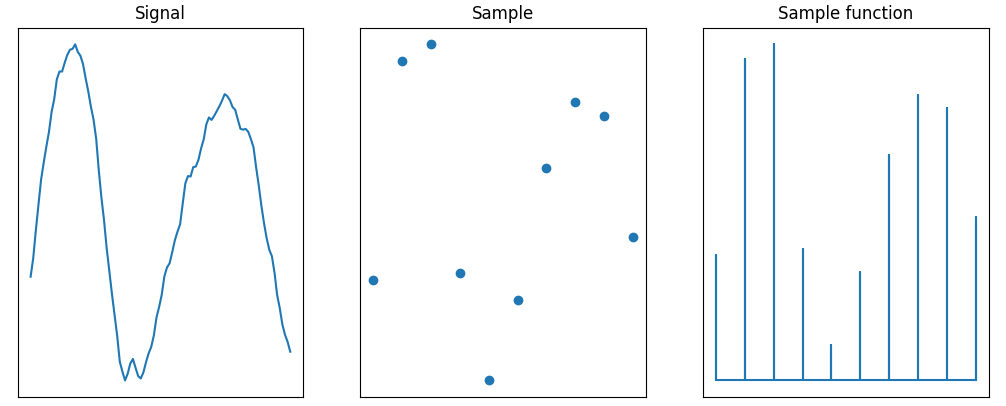
\includegraphics[scale=0.6]{sampled_function.png}
        \caption{A signal, the sample measured and the sample function generated.}
    \end{figure}
    We can approximate the average of the signal over some interval, \([x_j, x_k]\), as the average of the sample function over the same range, that is
    \begin{align*}
        \expected{f} &\approx \expected{f_S}\\
        &= \frac{1}{x_k - x_j} \int_{x_j}^{x_k} \dd{x} f_S(x)\\
        &= \frac{1}{x_k - x_j} \int_{x_j}^{x_k} \dd{x} f(x)\sum_{i}\delta(x - x_i)\\
        &= \frac{1}{x_k - x_j}\sum_i \int_{x_j}^{x_k} \dd{x} f(x)\delta(x - x_i)\\
        &= \frac{1}{x_k - x_j}\sum_{i=j}^{k} f(x_i)
    \end{align*}
    Assuming that \(x_i < x_{i + 1}\) so that \(x_i \in [x_j, x_k]\) if and only if \(i \in [j, k]\).
    
    \subsection{Infinite Comb}
    The most common case, which we will consider for the rest of the section, is that \(x_i\) are spaced evenly apart at some constant distance, \(\Delta x\), and that we have taken samples like this over all \(\reals\).
    Then the comb can be written as
    \[g(x) = \sum_{j\in\integers} \delta(x - j\Delta x).\]
    This is known as the \define{Shah function}, or \define{infinite comb}.
    Since \(f_S = fg\) we have that
    \[\FT[f_S] = \FT[fg] = \frac{1}{2\pi}\FT[f]\convolution\FT[g] = \frac{1}{2\pi}\tilde{f}\convolution\tilde{g},\]
    using the convolution theorem.
    For this to be useful we need to know what \(\tilde{g}\) is.
    
    We start by noting that \(g\) is periodic and therefore can be written as a Fourier series extended to all \(\reals\).
    The fundamental period of \(g\) is \(\Delta x\) so
    \[g(x) = \sum_{n\in\integers} c_ne^{2\pi inx/\Delta x}.\]
    Note the extra factor of 2 in the exponent as we are using the whole period, \(\ell = \Delta x\), instead of half the period, \(L = \Delta x / 2\).
    The Fourier coefficients are then
    \[c_n = \frac{1}{\Delta x}\int_{-\Delta x/2}^{\Delta x/2} \dd{x} \delta(x) e^{-2\pi inx/\Delta x} = \frac{1}{\Delta x}\]
    using the sifting property of the delta distribution.
    Hence
    \[g(x) = \frac{1}{\Delta x}\sum_{n\in\integers} e^{2\pi inx/\Delta x}.\]
    We can then use this to find the Fourier transform of \(g\).
    \begin{align*}
        \tilde{g}(k) &= \int_{-\infty}^{\infty} \dd{x} g(x)e^{-ikx}\\
        &= \int_{-\infty}^{\infty} \dd{x} \frac{1}{\Delta x} \sum_{n\in\integers} e^{2\pi inx/\Delta x}e^{-ikx}\\
        &= \frac{1}{\Delta x} \sum_{n\in\integers} \int_{-\infty}^{\infty} \dd{x} e^{ix(2\pi n/\Delta x - k)}\\
        &= \frac{2\pi}{\Delta x} \sum_{n\in\integers} \delta\left(k - \frac{2\pi n}{\Delta x}\right).
    \end{align*}
    Here we have used the integral representation of the delta distribution and the fact that the delta distribution is symmetric.
    We see that the Fourier transform of a comb is another comb in Fourier space.
    The spacing of \(\tilde{g}\) is \(2\pi/\Delta x\) which becomes wider as the spacing of \(g\) becomes narrower.
    This is just another example of the reciprocal relationship between a function and its Fourier transform.
    One consequence of this is if we have very fine sampling then we will end up with a wide range of wave numbers.
    
    We can now calculate \(\tilde{f}_S\):
    \begin{align*}
        \tilde{f}_S(k) &= \frac{1}{2\pi} (\tilde{f}\convolution\tilde{g})(k)\\
        &= \frac{1}{2\pi} \int_{-\infty}^{\infty} \dd{k'} \tilde{f}(k')g(k - k')\\
        &= \frac{1}{2\pi} \int_{-\infty}^{\infty} \dd{k'} \tilde{f}(k') \frac{2\pi}{\Delta x} \sum_{n\in\integers} \delta\left(k - k' - \frac{2\pi n}{\Delta x}\right)\\
        &= \frac{1}{\Delta x} \sum_{n\in\integers} \int_{-\infty}^{\infty} \dd{k'} \tilde{f}(k') \delta\left(k' - k + \frac{2\pi n}{\Delta x}\right)\\
        &= \frac{1}{\Delta x} \sum_{n\in\integers} \tilde{f}\left(k - \frac{2\pi n}{\Delta x}\right).
    \end{align*}
    
    \subsection{Constraints}
    We are looking for whether we can reconstruct \(f\) from \(f_S\), or equivalently if we can reconstruct \(\tilde{f}\) from \(\tilde{f}_S\).
    There are some constraints on when we can do this.
    The first is that the signal must be band limited.
    This means that \(\tilde{f}_S(k)\) must only be non-zero for \(k\in[-k_{\max}, k_{\max}]\) for some finite \(k_{\max}\in\reals\).
    This requirement is due to the next constraint which is that the sampling must be sufficiently fine.
    This is because we are representing the signal as periodic when we take a Fourier series.
    If the sampling isn't sufficiently fine then in Fourier space there will be overlaps at the edges which will then combine in the convolution to give the wrong \(\tilde{f}\).
    Therefore to have no overlap we require \(\Delta k \ge 2k_{\max}\).
    That is
    \[\frac{2\pi}{\Delta x} \ge 2k_{\max} \implies \frac{\pi}{\Delta x} \ge k_{\max}.\]
    The value \(k_{\text{Nyquist}} = \pi/\Delta x\) is known as the \define{Nyquist wavenumber}.
    
    \subsection{Interpolation of Samples}
    In reality we force the first constraint, that \(\tilde{f}_S\) is zero outside \([-k_{\max}, k_{\max}]\), with a filter in Fourier space.
    We use a top hat function with a height of 1 and a width \(2k_{\max}\).
    \(\tilde{f}_S(k)\Pi(k)\) is then automatically zero outside of \([-k_{\max}, k_{\max}]\) (assuming \(f_S\) is finite).
    We can find the original sampling function fairly easily from this:
    \begin{align*}
        f(x) &= \FT^{-1}[\tilde{f}_S\Pi](x)\\
        &= \left(\FT^{-1}[\tilde{f}_S] \convolution \FT^{-1}[\Pi]\right)(x)
        \shortintertext{defining \(T = \FT^{-1}[\Pi]\):}
        &= (f_S\convolution T)(x)\\
        &= ((fg) \convolution T)(x)\\
        &= \int_{-\infty}^{\infty} \dd{q} f(q)g(q) T(x - q)\\
        &= \int_{-\infty}^{\infty} \dd{q} f(q) \sum_{j\in\integers} \delta(q - j\Delta x) T(x - q)\\
        &= \sum_{j\in\integers} f(j\Delta x)T(x - j\Delta x)
    \end{align*}
    We already know what the inverse Fourier transform of a top hat is:
    \[T(x) = \FT^{-1}[\Pi](x) = \sinc(k_{\max}x) = \frac{\sin(k_{\max}x)}{k_{\max}x}.\]
    We then have that
    \[f(x) = \sum_{j\in\integers} f(j\Delta x)\sinc\left(k_{\max}(x - j\Delta x)\right).\]
    This is called the \define{sinc interpolation} of \(f\).
    Given that the constraints are met this is an exact recreation of \(f\).
    
    \section{DFTs and the FFT}
    \textit{This section is non-examinable.}
    
    \subsection{The Discrete Fourier Transform}
    Suppose we have a function, \(f\), which is periodic with period \(\ell\), representing some signal.
    Imagine also that we only know the value of \(f\) evaluated at some set of points, \(x_n = n\ell/N\), evenly spaced across this period.
    We also assume that \(f\) is band limited with a maximum wave number, \(k_{\max}\) satisfying the sampling theorem:
    \[\abs{k_{\max}} < \frac{\pi}{\Delta x} = \frac{\pi N}{\ell}.\]
    To express \(f\) as a Fourier series we would need to calculate the Fourier coefficients, which we denote \(f_k(k)\) here:
    \[f_k(k) = \frac{1}{\ell}\int_{0}^{\ell} \dd{x} f(x)e^{-ikx}.\]
    We can approximate this integral as a sum over the known values at \(x_n\):
    \[f_k(k) = \frac{1}{\ell}\sum_{n} f(x_n)e^{-ikx_n}\Delta x = \frac{1}{N}\sum_{n} f(x_n)e^{-ikx_n}.\]
    We will actually show that this is exactly the same as the integral assuming the sampling theorem is satisfied.
    The range of values that we sum over is unimportant as longs as the whole period is covered.
    For example we can define \(S_0\) to be the sum from 1 to \(N\) or \(S_N\) to be from 0 to \(N - 1\) as \(f(x_0) = f(x_N)\) so the difference between these two sums is
    \[S_0 - S_N = f(x_0)e^{-ikx_0} - f(x_N)e^{-ikx_N} = f(x_0)e^{ik(x_N - x_0)} = f(x_0)e^{ik\ell}.\]
    The allowed values of \(k\) are multiples of \(2\pi/\ell\) therefore
    \[S_0 - S_N = f(x_0)e^{-i2m\pi\ell/\ell} = f(x_0) = f(x_N).\]
    We are therefore to choose exactly which values to sum over.
    We define the \gls{dft} of the data to be
    \[f_k(k_m) = \frac{1}{N}\sum_{n=0}^{N-1} f(x_n)e^{-ik_mx_n},\]
    where \(k_m = 2\pi m/\ell\) and \(x_n = n\ell/N\).
    The inverse of this is
    \[f(x_j) = \sum_{m=0}^{N-1}f_k(k_m)e^{ik_mx_j}.\]
    To show this we insert the \gls{dft} into its inverse and we get
    \begin{align*}
        f(x_j) &= \frac{1}{N}\sum_{m=0}^{N-1}f_k(k_m)e^{ik_mx_j}\\
        &= \frac{1}{N}\sum_{m=0}^{N-1} \frac{1}{N}\sum_{n=0}^{N-1} f(x_n) e^{-k_mx_n} e^{ik_mx_j}\\
        &= \frac{1}{N}\sum_{m,n} f(x_n) e^{ik_m(x_j - x_n)}
        \shortintertext{now using the fact that \(k_mx_n = 2\pi mn/N\)}
        &= \frac{1}{N}\sum_{m,n} f(x_n) e^{2\pi im(j - n)/N}\\
        &= \frac{1}{N}\sum_{m, n} f(x_n) z^m
    \end{align*}
    where \(z = \exp[2\pi i(j - n)/N]\).
    When \(j = n\) we have \(z = 1\) so \(\sum_m z^m = N\).
    When \(j \ne n\) the sum is zero.
    To show this consider
    \[z\sum_{m} z^m = z(1 + z + z^2 + \dotsb + z^{N-1}) = z + z^2 + z^3 + \dotsb + z^{N} = z^N - 1 + \sum_m z^m.\]
    However \(z^N = 1\) so we have
    \[z\sum_{m} z^m = \sum_{m} z^m.\]
    Since \(z \ne 1\) we must have that \(\sum_mz^m = 0\).
    Therefore
    \[\sum_m z^m = N\delta_{jn}.\]
    Thus
    \begin{align*}
        f(x_j) &= \frac{1}{N}\sum_{m, n} f(x_n)z^m\\
        &= \frac{1}{N}\sum_n f(x_n)N\delta_{jn}\\
        &= f(x_j)
    \end{align*}
    
    \subsection{The Fast Fourier Transform}
    \glspl{dft} are common in data compression as they allow us to represent a large amount of data as a small sample of the whole data set.
    However in practical applications there are still often a huge number of data points, \(x_n\).
    For example, a CD samples at \SI{44.1}{\kilo\hertz}.
    This means that for a three minute song there are 7938000 samples.
    The naive implementation of the \gls{dft}, that is just implementing the sums, is \(\order{N^2}\).
    Fortunately the \gls{fft} algorithm exists and allows us to implement a \gls{dft} in \(\order{N\log N}\).
    This may not sound that much better but suppose we have \(N = \nu,
    e9\) data points and can perform one operation per nanosecond.
    Then the naive implementation takes \(N^2 = \num{e18}\) operations which corresponds to \(\SI{e18}{\nano\second} = \SI{31.2}{years}\).
    The \gls{fft} on the other hand takes \(N\log N = \num{30e9}\) operations which corresponds to \(\SI{30e9}{\nano\second} = \SI{30}{\second}\).
    This is clearly a huge improvement.
    
    To implement the \gls{fft} we define \(W_N = \exp[-2\pi i/N]\).
    Computing the \gls{dft} then entails calculating
    \[F_m = \sum_{n=0}^{N-1}f_nW_N^{nm}.\]
    The \(N\) terms in the sum as well as \(N\) multiplications of the complex numbers \(f_n\) and \(W_N\) gives the \(N^2\) operations that lead to the naive implementation being \(\order{N^2}\).
    The \gls{fft} exploits two symmetries of \(W_N\):
    \begin{itemize}
        \item Complex conjugate symmetry:
        \[W_N^{k(N-n)} = W_N^{kN}W_N^{-kn} = W^{-Kn} = (W_N^{kn})^*.\]
        \item Periodicity in \(n\):
        \[W_N^{k(n + N)} = W_N^{kn}W_N^{kN} = W_N^{kn}\]
        and periodicity in \(k\):
        \[W_N^{(k + N)n} = W_N^{kn}W_N^{nN} = W_N^{kn}.\]
    \end{itemize}
    The steps for deriving the \gls{fft} are as follows:
    \begin{enumerate}
        \item Build a big \gls{dft} from smaller ones.
        \item Assume that \(N = 2^p\) for some \(p\in\integers\) (if this isn't the case it turns out that we can just add zeros to our data set until it is, this is called the packing theorem).
        \item Split the sum into even and odd indices.
    \end{enumerate}
    Making the assumption that \(N = 2^p\) and splitting the sum we have
    \[F_m = \sum_{n=0}^{N-1}f_nW_N^{nm} = \sum_{n~\text{even}}f_nW_N^{nm} + \sum_{n~\text{odd}}f_nW_N^{nm}.\]
    We can write the even and odd indices as \(2r\) and \(2r+1\) respectively for \(r = 0, 1, \dots, N/2 - 1\).
    Doing this we have
    \begin{align*}
        F_m &= \sum_{r=0}^{N/2-1}f_{2r}W_N^{2rm} + \sum_{r=0}^{N/2-1}f_{2r+1}W_N^{(2r+1)m}\\
        &= \sum_{r=0}^{N/2-1}f_{2r}W_N^{2rm} + \sum_{r=0}^{N/2-1}f_{2r+1}W_N^{2rm+m}\\
        &= \sum_{r=0}^{N/2-1}f_{2r}W_N^{2rm} + W_{N}^m\sum_{r=0}^{N/2-1}f_{2r+1}W_N^{2rm}\\
        &= \sum_{r=0}^{N/2-1}f_{2r}(W_N^2)^rm + W_N^m\sum_{r=0}^{N/2-1}f_{2r+1}(W_N^2)^{rm}\\
    \end{align*}
    Now we note that
    \[W_N^2 = (e^{-2\pi i/N})^2 = e^{-4\pi i/N} = e^{-2\pi i/(N/2)} = W_{N/2}.\]
    Hence
    \[F_m = \sum_{r=0}^{N/2 - 1} f_{2r}W_{N/2}^{rm} + W_N^m\sum_{r=0}^{N/2-1} f_{2r+1}W_{N/2}^{rm} = F_{em} + W_N^mF_{om}\]
    where \(F_{em}\) and \(F_{om}\) are the \glspl{dft} of the data sets of only the even and odd indices respectively.
    In the case that there is more than 1 data point in each of these data sets we can perform the \gls{fft} on these again recursively to get the \gls{dft} of the odd and even sets.
    We can keep doing this until the data sets contain only one element and the \gls{dft} of a single data point is just that data point.
    \begin{figure}[ht]
        \centering
        \begin{tikzpicture}
            \foreach \x in {0, ..., 3} {
                \tikzmath{\y=int(2*\x);}
                \node (Fl) at (0, 8 - 0.5*\x) {\(F_{\y}\)};
                \node (Fr) at (2, 8 - 0.5*\x) {\(F_{e\x}\)};
                \draw (Fl) -- ($(Fl) + (0.5, 0)$);
                \draw (Fr) -- ($(Fr) - (0.5, 0)$);
                \draw (Fr) -- ($(Fr) + (3, 0)$);
                \draw ($(Fr) + (1, 0)$) -- ($(Fr) + (2.3, -3)$);
                \node[right] at ($(Fr) + (3, 0)$) {\(F_{e\x} + W_{8}^{\x}F_{o\x} = F_{\x}\)};
                \tikzmath{int \y; \y=2*\x+1;}
                \node (Fl) at (0, 5 - 0.5*\x) {\(F_{\y}\)};
                \node (Fr) at (2, 5 - 0.5*\x) {\(F_{o\x}\)};
                \draw (Fl) -- ($(Fl) + (0.5, 0)$);
                \draw (Fr) -- ($(Fr) - (0.5, 0)$);
                \draw (Fr) -- ($(Fr) + (3, 0)$);
                \draw ($(Fr) + (1, 0)$) -- ($(Fr) + (2.3, 3)$);
                \tikzmath{int \z; \z = \x+4;}
                \node[right] at ($(Fr) + (3, 0)$) {\(F_{e\x} + W_{8}^{\z}F_{o\x} = F_{\z}\)};
            }
            \draw (0.5, 8.2) rectangle (1.5, 6.3);
            \draw (0.5, 5.2) rectangle (1.5, 3.3);
            \node[align=center, text width=1] at (0.7, 7.25) {\(N/2\) DFT even};
            \node[align=center, text width=1] at (0.7, 4.25) {\(N/2\) DFT odd};
        \end{tikzpicture}
        \caption{Creating a Fourier transform from two smaller Fourier Transforms, \(N = 8\) case.}
        \label{fig:fft example}
    \end{figure}
    We said before that the \gls{fft} is \(\order{N\log N}\).
    Now we can show that this is true.
    Figure~\ref{fig:fft example} shows a \gls{fft} for \(N = 8\).
    We see that we have to perform two \glspl{dft} with \(N/2\) elements.
    We also have to do \(N\) sums.
    Performing each \gls{dft} with the naive algorithm this means there are
    \[2\left(\frac{N}{2}\right)^2 + N = \frac{N^2}{2} + N\]
    operations.
    If instead we compute the two \glspl{dft} by \glspl{fft}, but all later \glspl{dft} by the naive algorithm then there are
    \[2\left(2\left(\frac{N}{4}\right)^2 + \frac{N}{2}\right) = \frac{N^2}{4} + 2N\]
    operations.
    If we perform all \glspl{dft} as \glspl{fft} then we end up splitting the data \(p = \log_2 N\) times.
    There are then
    \[\frac{N^2}{2^p} + pN = \frac{N^2}{N} + N\log_2N\]
    operations, which scales as \(\order{N\log_2 N}\).
    
    \section{Ordinary Differential Equations}
    \subsection{When Does a Fourier Transform Exist?}
    \textit{This subsection is non-examinable}
    
    So far we have assumed that the Fourier transform of any function, \(f\), exists.
    Strictly speaking this is contingent on
    \[\tilde{f}(k) = \int_{-\infty}^{\infty} \dd{x} f(x)e^{-ikx}\]
    converging, meaning this value must be defined and finite.
    The following set of conditions, known as the \define{Dirichlet conditions} are, together, necessary and sufficient for the Fourier transform of \(f\) to exist:
    \begin{enumerate}
        \item The function must be single valued and have a finite number of finite discontinuities.
        \item The function must have a finite number of maxima and minima.
        \item The function must be absolutely integrable, meaning that
        \[\int_{-\infty}^{\infty} \abs{f(x)} \dd{x}\]
        converges.
    \end{enumerate}
    The conditions for the Fourier series to exist are similar but include \(f\) being periodic:
    \begin{enumerate}
        \item The function must be periodic.
        \item The function must have a finite number of finite discontinuities.
        \item The function must have a finite number of maxima and minima within one period.
        \item The function must be absolutely integrable over one period, meaning that
        \[\int_{-L}^{L} \abs{f(x)} \dd{x}\]
        must converge assuming a period of \(2L\).
    \end{enumerate}
    In practice for the sort of functions that we use in physics it is normally the last of these conditions, absolute integrability, that is failed if any.
    For example consider \(f(x) = e^x\).
    We know that all but the last Dirichlet condition are satisfied for the Fourier transform:
    \[\int_{-\infty}^{\infty} \abs{e^x} \dd{x} = 2\int_{0}^{\infty} e^x \dd{x} = 2[e^x]_{0}^{\infty} = \infty.\]
    We will continue to assume that Fourier transforms exist for functions that we are interested in.
    
    \subsection{Fourier Transforms of Derivatives}
    Let \(f\) be a function with a Fourier transform.
    Then
    \[\dv{f}{x} = \dv{x}\frac{1}{2\pi} \int_{-\infty}^{\infty} \dd{k} \tilde{f}(k) e^{ikx} = \frac{1}{2\pi} \int_{-\infty}^{\infty} \dd{k} \tilde{f}(k) \dv{x} e^{ikx} = \frac{1}{2\pi} \int_{-\infty}^{\infty} \dd{k} ik \tilde{f}(k)e^{ikx}.\]
    If we identify \(\FT[f'] = ik\tilde{f}\) then we see that
    \[\FT[f'] = ik\FT[f].\]
    The \(p\)th derivative is then
    \[\FT[f^{(p)}] = (ik)^p\FT[f].\]
    
    \subsection{Driven, Damped, Simple Harmonic Motion}
    Consider a mass, \(m\), attached to a spring with spring constant \(k\).
    If the mass is moved slightly from equilibrium it will undergo simple harmonic motion.
    If the mass is in a viscous fluid (such as air) it will also experience a resistive force proportional to its velocity.
    We can also drive the oscillation with some force, \(F(t)\).
    This leads to a differential equation
    \[m\ddot{z} = -kz - D\dot{z} + F(t)\]
    where \(D\) is a constant of proportionality for the damping term.
    All constants are positive.
    Dividing through by the mass and rearranging we have
    \[\ddot{z} + \frac{D}{m}\dot{z} + \frac{k}{m}z = \frac{1}{m}F(t).\]
    We now define \(\gamma = D/m\), \(\omega_0^2 = k/m\), and \(f(t) = F(t)/m\).
    This allows us to write this differential equation in the standard form for a linear second order \gls{ode}:
    \[\ddot{z} + \gamma\dot{z} + \omega_0^2z = f(t).\]
    This can be solved without Fourier analysis in some specific cases but it is easier with Fourier analysis and Fourier analysis allows us to find a general solution.
    
    \subsubsection{Method 1: Real Periodic Driving Force}
    Suppose
    \[f(t) = A\cos(\omega t).\]
    We make the ansatz that
    \[z(t) = a\cos(\omega t) + b\sin(\omega t)\]
    for some constants \(a\) and \(b\) to be calculated.
    Therefore
    \[\dot{z} = -a\omega\sin(\omega t) + b\omega\cos(\omega t), \qquad\text{and}\qquad \ddot{z} = -a\omega^2\cos(\omega t) - b\omega^2\sin(\omega t).\]
    Substituting these into the original differential equation we get
    \[-a\omega^2\cos(\omega t) - b\omega^2\sin(\omega t) - a\omega\gamma\sin(\omega t) + b\omega\gamma\cos(\omega t) + a\omega_0^2\cos(\omega t) + b\omega_0^2\sin(\omega t) = A\cos(\omega t).\]
    In order for the right hand side to be a pure cosine term we equate coefficients and require that
    \[-a\omega^2 + b\omega\gamma + a\omega_0^2 = a(\omega_0^2 - \omega^2) + b\omega\gamma = A\]
    and
    \[-b\omega^2 - a\omega\gamma + b\omega_0^2 = b(\omega_0^2 - \omega^2) -\omega\gamma = 0.\]
    We can succinctly write these two conditions with one matrix equation:
    \[
        \begin{pmatrix}
            \omega_0^2 - \omega^2 & \gamma\omega\\
            -\gamma\omega & \omega_0^2 - \omega^2
        \end{pmatrix}
        \begin{pmatrix}
            a\\ b
        \end{pmatrix}
        =
        \begin{pmatrix}
            A\\ 0
        \end{pmatrix}
        .
    \]
    This can be solved by noting that the inverse of a \(2\times 2\) matrix is given by
    \[
        \begin{pmatrix}
            \zeta & \chi\\
            \xi & \eta
        \end{pmatrix}
        ^{-1} =
        \frac{1}{\zeta\eta - \chi\xi}
        \begin{pmatrix}
            \eta & -\chi\\
            -\xi & \zeta
        \end{pmatrix}
        .
    \]
    Hence
    \begin{align*}
        \begin{pmatrix}
            a\\ b
        \end{pmatrix}
        &=
        \frac{1}{(\omega^2 - \omega_0^2)^2 + \gamma^2\omega^2}
        \begin{pmatrix}
            \omega_0^2 - \omega^2 & -\gamma\omega\\
            \gamma\omega & \omega_0^2 - \omega^2
        \end{pmatrix}
        \begin{pmatrix}
            A\\ 0
        \end{pmatrix}
        \\
        &= \frac{1}{(\omega_0^2 - \omega^2)^2 + \gamma^2\omega^2}
        \begin{pmatrix}
            (\omega_0^2 - \omega^2)A\\ \gamma\omega A
        \end{pmatrix}
    \end{align*}
    Which gives us
    \[a = (\omega_0^2 - \omega^2),\qquad\text{and}\qquad b = \gamma\omega A.\]
    Hence the solution is
    \[z = \frac{A[(\omega_0^2 - \omega^2)\cos(\omega t) + \gamma\omega\sin(\omega t)]}{(\omega_0^2 - \omega^2)^2 + \gamma^2\omega^2}\].
    Using the trigonometric identity
    \[\cos(\omega t + \alpha) = \cos(\omega t)\cos(\alpha) - \sin(\omega t)\sin(\alpha)\]
    We see that we can express the numerator of the solution as
    \[\cos(\omega t - \alpha) = (\omega_0^2 - \omega^2)\cos(\omega t) - \gamma\omega\sin(\omega t)\]
    Equating coefficients between this and the trig identity we have
    \[\cos\alpha = \omega_0^2 - \omega^2\qquad\text{and}\qquad \sin\alpha = \gamma\omega.\]
    So
    \[\alpha = \arctan\left(\frac{\gamma\omega}{\omega_0^2 - \omega^2}\right).\]
    We see that the oscillation is then periodic with amplitude
    \[\frac{A}{(\omega_0^2 - \omega^2)^2 + \gamma^2\omega^2}\]
    and the oscillation lags behind the force by a phase difference of \(\alpha\).
    
    \subsection{Method 1: Complex Periodic Driving Force}
    The force \(A\cos(\omega t)\) can be written as \(\Re[Ae^{i\omega t}]\).
    Since the differential equation in question is linear we can solve it for \(f(t) = e^{i\omega t}\) and simply take the real part at the end.
    We make the ansatz that \(z(t) = Ce^{i\omega t}\).
    Thus
    \[\dot{z} = i\omega Ce^{i\omega t}, \qquad\text{and}\qquad \ddot{z} = -\omega^2Ce^{i\omega t}.\]
    Substituting these into the differential equation we get
    \[-\omega^2Ce^{i\omega t} + i\gamma\omega Ce^{i\omega t} + \omega_0^2Ce^{i\omega t} = Ae^{i\omega t}\]
    so we have that
    \[C = \frac{A}{\omega_0^2 - \omega^2 + i\gamma\omega}.\]
    Since \(A\in\complex\) we can write \(A = \abs{A}e^{i\varphi}\).
    If we also define \(B = \omega_0^2 - \omega^2 + i\gamma\omega\) then we can write \(B = \abs{B}e^{i\alpha}\) where
    \[\abs{B}^2 = (\omega_0^2 - \omega^2)^2 + \gamma^2\omega^2.\]
    We also have
    \[\alpha = \arctan\left(\frac{\gamma\omega}{\omega_0^2 - \omega^2}\right).\]
    Thus the solution is
    \[z(t) = \Re\left[\frac{\abs{A}}{\abs{B}}e^{i\omega t + \varphi - \alpha}\right].\]
    This is the same solution as we got with the last method but we reached it considerably quicker.
    
    \subsection{Method 3: Fourier Analysis}
    In the frequency domain we have
    \[\FT[z](\omega) = \tilde{z}(\omega), \qquad\text{and}\qquad \FT[f](\omega) = \tilde{f}(\omega).\]
    We can use the Fourier transform of the derivatives to turn the differential equation into a purely algebraic equation:
    \[\FT[\dot{z}](\omega) = i\omega\tilde{z}(\omega), \qquad\text{and}\qquad \FT[\ddot{z}](\omega) = -\omega^2\tilde{z}(\omega).\]
    Thus if we Fourier transform the entire differential equation, using the fact that the Fourier transform is a linear operation, we have
    \[-\omega^2\tilde{z}(\omega) + i\omega\gamma\tilde{z}(\omega) + \omega_0^2\tilde{z}(\omega) = \tilde{f}(\omega).\]
    Hence
    \[\tilde{z}(\omega) = \frac{\tilde{f}}{\omega_0^2 - \omega^2 + i\gamma\omega}.\]
    So far this is completely general.
    Now suppose that \(f(t) = Ae^{i\Omega t}\).
    We can easily calculate the Fourier transform of this:
    \begin{align*}
        \tilde{f}(\omega) &= A \int_{0}^{\infty} \dd{t} e^{i\Omega t}e^{-\omega t}\\
        &= A \int_{0}^{\infty} \dd{t} e^{it(\Omega - \omega)}\\
        &= 2\pi A\delta(\omega - \Omega).
    \end{align*}
    Hence
    \begin{align*}
        z(t) &= \frac{1}{2\pi} \int_{0}^{\infty} \dd{\omega} \tilde{z}(\omega)e^{i\omega t}\\
        &= \frac{1}{2\pi} \int_{0}^{\infty} \dd{\omega} \frac{\tilde{f}(\omega)}{\omega_0^2 - \omega^2 + i\gamma\omega}e^{i\omega t}\\
        &= A\int_{0}^{\infty} \frac{\delta(\omega - \Omega)}{\omega_0^2 - \omega^2 + i\gamma\omega}\\
        &= \frac{Ae^{i\Omega t}}{\omega_0^2 - \omega^2 + i\gamma\omega}\\
        &= \frac{\abs{A}}{\abs{B}}e^{i\Omega t + \varphi - \alpha}.
    \end{align*}
    So we arrive at the same answer as before.
    This method was at least easy as the other methods and doesn't rely on an initial ansatz.
    This method can also be applied in the same way to any linear differential equation.
    
    \section{Linear Differential Equations}
    \subsection{Periodic Forces}
    When using the Fourier transform approach to solve the equation
    \[\ddot{z} + \gamma\dot{z} + \omega_0^2z = f(t)\]
    we didn't assume that the driving force, \(f\), or the response, \(z\), was periodic.
    In the case that \(f\) is periodic with period \(T\), such that \(f(t + T) = f(t)\) for all \(t\), we can expand \(f\) and \(z\) as Fourier series:
    \[z(t) = \sum_n c_ne^{i\omega_n t}, \qquad\text{and}\qquad f(t) = \sum_n d_ne^{i\omega_n t}.\]
    Calculating derivatives of \(z\) we have
    \[\dot{z}(t) = \sum_n c_n i\omega_n e^{i\omega_n t}, \qquad\text{and} \qquad \ddot{z}(t) = -\sum_n c_n\omega_n^2 e^{i\omega_n t}.\]
    Thus the differential equation becomes
    \[-\sum_n c_n\omega_n^2 e^{i\omega_n t} + \gamma \sum_n c_n i\omega_n e^{i\omega_n t} + \omega_0^2 \sum_n c_ne^{i\omega_n t} = \sum_n d_ne^{i\omega_n t}\]
    which simplifies to
    \[\sum_n (\omega_0^2 - \omega_n^2 + i\gamma\omega_n)c_n e^{i\omega_n t} = \sum_n d_n e^{i\omega_n t}.\]
    Using the orthogonality of Fourier modes we must have that
    \[d_n = (\omega_n^2 - \omega_0^2 + i\gamma\omega_n)c_n \implies c_n = \frac{d_n}{(\omega_0^2 - \omega_n^2) + i\gamma\omega_n}\]
    So assuming that we can calculate \(d_n\) we can easily find \(z\) using the Fourier series with the coefficients \(c_n\) given above.
    
    \subsection{Linear Differential Equations}
    The most general \define{linear differential equation} can be written as
    \[Lz(t) = f(t).\]
    Here \(L\) is a \define{linear differential operator}, this means that for constants \(a\) and \(b\) and functions \(z_1\) and \(z_2\)
    \[L[az_1(t) + bz_2(t)] = aLz_1(t) + bLz_2(t).\]
    For example, the damped harmonic oscillator can be written like this with
    \[L = \dv[2]{t} + \gamma\dv{t} + \omega_0^2.\]
    Given a linear differential equation like above the \define{homogeneous equation} is
    \[Lz_h(t) = 0.\]
    This is important because if \(z_h\) is a solution to the homogeneous equation and \(z\) is a solution to the inhomogeneous equation then \(z + z_h\) is the most general solution to the inhomogeneous equation:
    \[L(z(t) + z_h(t)) = Lz(t) + Lz_h(t) = Lz(t) + 0 = f(t).\]
    Therefore we always need to solve the homogenous equation to find the most general solution.
    
    \begin{example}
        Suppose we want to solve the damped, driven harmonic oscillator.
        We try an oscillating solution, \(z_h\propto e^{i\omega t}\), for the \define{complementary function} (the solution to the homogenous equation).
        Substituting this into the differential equation and simplifying we get the \define{auxialiary equation}:
        \[\omega^2 - i\gamma\omega - \omega_0^2 = 0.\]
        This is a quadratic equation in \(\omega\) and has the solution
        \[\omega = \frac{i\gamma \pm \sqrt{i\gamma^2 + 4\omega_0^2}}{2}.\]
        There are three cases that we can consider:
        \begin{itemize}
            \item \textit{Under damped} -- \(\gamma/2 < \omega_0\), in this case
            \[z(t) = e^{i\gamma t/2}(Ae^{i\Omega t} + Be^{-i\Omega t})\]
            where \(\Omega = \sqrt{-\gamma^2/4 + \omega_0^2}\in\reals\).
            In this case the oscillations slowly die away.
            \item \textit{Over damped} -- \(\gamma/2 > \omega_0\), in this case
            \[z(t) = e^{i\gamma t/2}(Ae^{\Omega't} + Be^{-i\Omega' t})\]
            where \(\Omega' = \sqrt{\gamma^2/4 - \omega_0^2}\in\reals\).
            In this case there is no oscillation, there is instead exponential decay.
            \item \textit{Critically damped} -- \(\gamma/2 = \omega_0\), in this case
            \[z(t) = e^{i\gamma t/2}(A + Bt).\]
            In this case the system returns to equilibrium rapidly and stays there.
        \end{itemize}
    \end{example}
    
    \subsection{Convolution Approach}\label{sec:convolution approach}
    Consider the un-damped harmonic oscillator:
    \[\dv[2]{z}{t} + \omega_0^2z = f(t).\]
    Taking the Fourier transform we have
    \[-\omega^2\tilde{z}(\omega) - \omega_0^2\tilde{z}(\omega) = \tilde{f}(\omega) \implies \tilde{z}(\omega) = -\frac{\tilde{f}(\omega)}{\omega_0^2 + \omega^2}.\]
    So far this is the same as the Fourier approach where we saw the solution was
    \[z(t) = -\frac{1}{2\pi}\int_{-\infty}^{\infty} \dd{\omega} \frac{\tilde{f}(\omega)}{\omega_0^2 + \omega^2}e^{i\omega t}.\]
    It is possible that this integral will be difficult to do.
    We may be able to simplify this by defining
    \[\tilde{g}(\omega) = -\frac{1}{\omega_0^2 + \omega^2}\]
    so \(\tilde{z}(\omega) = \tilde{f}(\omega)\tilde{g}(\omega)\).
    By the convolution theorem this means that
    \[z(t) = (f\convolution g)(t) = \int_{-\infty}^{\infty} \dd{t'}f(t')g(t - t').\]
    So now we simply need to find \(g\) and evaluate this integral.
    It can be shown that
    \[g(t) = -\frac{e^{-\omega_0\abs{t}}}{2\omega_0}.\]
    It is relatively simple to show that this is correct:
    \begin{align*}
        \tilde{g}(\omega) &= \int_{-\infty}^{\infty} \dd{t} g(t) e^{-i\omega t}\\
        &= -\int_{-\infty}^{\infty} \dd{t} \frac{e^{-\omega_0\abs{t}}}{2\omega_0} e^{-i\omega t}\\
        &= -\frac{1}{2\omega_0}\int_{-\infty}^{\infty} \dd{t} e^{-\omega_0\abs{t} - i\omega t}\\
        &= -\frac{1}{2\omega_0}\int_{-\infty}^{0} \dd{t} e^{-\omega_0\abs{t} - i\omega t} -\frac{1}{2\omega_0} \int_{0}^{\infty} \dd{t} e^{-\omega_0\abs{t} - i\omega t}\\
        &= -\frac{1}{2\omega_0}\int_{-\infty}^{0} \dd{t} e^{\omega_0t - i\omega t} - \frac{1}{2\omega_0}\int_{0}^{\infty} \dd{t} e^{-\omega_0 t - i\omega t}\\
        &= \frac{1}{2\omega_0}\left[\frac{e^{\omega_0 t - i\omega t}}{i\omega - \omega_0}\right]_{-\infty}^{0} + \frac{1}{2\omega_0}\left[\frac{e^{-\omega_0 t - i\omega t}}{\omega_0 + i\omega}\right]_0^{\infty}\\
        &= \frac{1}{2\omega_0}\frac{1}{i\omega - \omega_0} - \frac{1}{2\omega_0}\frac{1}{i\omega + \omega_0}\\
        &= \frac{1}{2\omega_0}\frac{(i\omega + \omega_0) - (i\omega - \omega_0)}{(i\omega - \omega_0)(i\omega + \omega_0)}\\
        &= \frac{1}{2\omega_0}\frac{2\omega_0}{-\omega^2 - \omega_0^2}\\
        &= -\frac{1}{\omega_0^2 + \omega^2}
    \end{align*}
    Thus
    \[z(t) = -\frac{1}{2\omega_0}\int_{-\infty}^{\infty} \dd{t'} f(t')e^{-\omega_0\abs{t - t'}}.\]
    Suppose \(f(t) = A\cos(\Omega t)\).
    Then
    \begin{align*}
        z(t) &= \frac{1}{2\omega_0}\int_{-\infty}^{\infty} \dd{t'}f(t - t')e^{i\omega_0\abs{t'}}\\
        &= \frac{1}{2\omega_0}\left[\int_{-\infty}^{0} \dd{t'} f(t - t')e^{-i\omega_0t'} + \int_{0}^{\infty} \dd{t'} f(t - t')e^{i\omega_0t'}\right]
        \shortintertext{for the first integral let \(t'\to-t'\) so \(\dd{t'}\to-\dd{t'}\) and \((-\infty, 0)\to (\infty, 0)\):}
        &= \frac{1}{2\omega_0} \left[-\int_{\infty}^{0} \dd{t'}f(t + t')e^{i\omega_0t'} + \int_{0}^{\infty} \dd{t'} f(t - t')e^{i\omega_0t'} \right]\\
        &= \frac{1}{2\omega_0} \int_{0}^{\infty} \dd{t'} [f(t + t') + f(t - t')]e^{i\omega_0t'}\\
        &= \frac{A}{2\omega_0} \int_{0}^{\infty} \dd{t'} [\cos(\Omega(t + t')) + \cos(\Omega(t - t'))]e^{i\omega_0t}\\
        &= \frac{A}{2\omega_0} \int_{0}^{\infty} \dd{t'} 2\cos(\Omega t)\cos(\Omega t')e^{i\omega_0t'}\\
        &= \frac{A\cos(\Omega t)}{\omega_0} \int_{0}^{\infty} \dd{t'}\cos(\Omega t')e^{i\omega_0t'}
        \shortintertext{integrating by parts gives}
        &= \frac{A\cos(\Omega t)}{\omega_0^2 - \omega^2}.
    \end{align*}

    \section{Green's Functions}
    For a linear differential equation,
    \[Ly(t) = f(t),\]
    the \define{Green's function}, \(G\), is defined as the solution to
    \[LG(t, T) = \delta(t - T).\]
    The Green's function tells us the response of the system to an impulse at \(t = T\).
    In general we can write \(f\) as
    \[f(t) = \int\dd{q}f(q)\delta(t - q),\]
    which is a superposition of spikes weighted by \(f\).
    Or we can write \(f\) as
    \[f(t) = \frac{1}{2\pi} \int_{-\infty}^{\infty} \dd{\omega} \tilde{f}(\omega)e^{i\omega t},\]
    which is a superposition of waves weighted by \(\tilde{f}\).
    
    One example of this may be in electromagnetism.
    Poisson's equation for the potential is
    \[\laplacian\varphi = -\frac{\rho}{\varepsilon_0}.\]
    The Green's function for this is
    \[G(\vv{r}, \vv{r_q}) = -\frac{1}{4\pi\abs{\vv{r} - \vv{r_q}}}.\]
    This is the same as the potential due to a point charge, \(-\varepsilon_0\), at \(\vv{r_q}\).
    
    Given a Green's function for a particular differential equation how do we use it to find the solution?
    Starting with the definition of the Green's function,
    \[LG(t, T) = \delta(t - T),\]
    we can multiply through by \(f(T)\) to get
    \[LG(t, T)f(T) = \delta(t - T)f(T).\]
    Note that \(L\) acts only on \(t\), not on \(T\) so any function independent of \(t\) commutes with \(L\).
    Integrating we have
    \[\int \dd{T} LG(t, T)f(T) = \int \dd{T} \delta(t - T)f(T) = f(t)\]
    where we have used the sifting property of the delta distribution in the last step.
    Now notice that \(L\) and \(\int\dd{T}\) commute so
    \[L\int\dd{T}G(t, T)f(T) = f(t).\]
    Thus we have found a function, \(\int\dd{T}G(t, T)f(T)\), that when acted on by \(L\) gives \(f(t)\).
    Thus we conclude that
    \[y(t) = \int\dd{T}G(t, T)f(T).\]
    So we see that the solution is a superposition of the systems response to an impulse weighted by \(f\).
    
    \subsection{Calculating Green's Functions}
    The most general second order linear differential equation has
    \[L = \dv[2]{x} + a_1(x)\dv{x} + a_0(x).\]
    Here \(a_1\) and \(a_0\) are continuous functions and
    \[Ly(x) = f(x).\]
    The method for finding the Green's function is always the same:
    \begin{enumerate}
        \item Replace \(f(x)\) with an impulse, \(\delta(x - X)\).
        \item Split the range into intervals, \(x < X\) and \(x > X\).
        For both of these intervals \(x \ne X\) so \(LG = \delta(x - X) = 0\).
        Solve this for \(G\).
        \item At \(x = X\) impose continuity of \(G(x, X)\) so
        \[\lim_{x\to X^-} G(x, X) = \lim_{x\to X^+}G(x, X).\]
        \item At \(x = X\) \(\inlinedv{G}{x}\) is discontinuous.
        We show this here:
        \[LG(x, X) = \delta(x - X) \implies \pdv[2]{G}{x} + a_1(x)\pdv{G}{x} + a_0(x) = \delta(x - X).\]
        We now use the fact that \(\delta\) can be normalised:
        \[\lim_{\varepsilon\to 0}\int_{X - \varepsilon}^{X + \varepsilon} LG(x, X)\dd{x} = \lim_{\varepsilon\to 0}\int_{X - \varepsilon}^{X + \varepsilon} \delta(x - X) \dd{x} = 1.\]
        Then
        \[\lim_{\varepsilon\to 0}\left[\int_{X - \varepsilon}^{X + \varepsilon} \pdv[2]{G}{x} \dd{x} + \int_{X - \varepsilon}^{X + \varepsilon} a_1(x)\pdv{G}{x}\dd{x} + \int_{X - \varepsilon}^{X + \varepsilon}a_0(x)\dd{x}\right] = 1.\]
        Considering this a term at a time and using the fact that for a continuous function, \(g\),
        \[\lim_{a\to b}\int_a^b g(x)\dd{x} = 0\]
        we have
        \[\lim_{\varepsilon\to 0} \int_{X - \varepsilon}^{X + \varepsilon}a_0(x)\dd{x} = 0,\]
        and
        \[\lim_{\varepsilon\to 0} \int_{X - \varepsilon}^{X + \varepsilon} a_1(x)\pdv{G}{x}\dd{x} = \lim_{\varepsilon\to 0}\left[ \left[a_1(X)G(x, X)\right]_{X - \varepsilon}^{X + \varepsilon} \int_{X - \varepsilon}^{X + \varepsilon} G\dv{a_1}{x} \dd{x} \right] = 0\]
        since \(\inlinedv{a_1}{x}\) and \(G\) are continuous.
        Finally
        \[\lim_{\varepsilon\to 0} \int_{X - \varepsilon}^{X + \varepsilon} \pdv[2]{G}{x}\dd{x} = \lim_{\varepsilon\to 0} \left[\pdv{G}{x}\right]_{X - \varepsilon}^{X + \varepsilon} = \lim_{\varepsilon\to 0}\left(\pdvat{G}{x}{X + \varepsilon} - \pdvat{G}{x}{X - \varepsilon}\right) = 1.\]
        This can only be non-zero if \(\partial_x G\) is discontinuous at \(x = X\).
    \end{enumerate}
    \begin{example}
        Suppose we want to solve
        \[\dv[2]{y}{x} + y = x,\]
        with the boundary conditions \(y(0) = y(\pi/2) = 0\).
        Therefore we only care about the function between the points \(0\) and \(\pi/2\).
        So in the second step we split the range into the intervals \([0, X)\) and \((X, \pi/2]\).
        In these two intervals we solve \(LG = \delta(x - X) = 0\) and we recognise that this corresponds to an un-damped, un-driven, harmonic oscillator so the solutions in these regions are
        \[
            G(x, X) = 
            \begin{cases}
                A(X)\sin(x) + B(X)\cos(x), & x < X,\\
                C(X)\sin(x) + D(X)\cos(x), & x > X.
            \end{cases}
        \]
        Notice that the coefficients are functions of \(X\) as the position of the spike affects the solution.
        Imposing the boundary conditions we have that at \(x = 0\) \(G(0, X) = 0\) so \(B(X) = 0\).
        Similarly at \(x = \pi/2\) \(G(\pi/2, X) = 0\) so \(C(X) = 0\).
        Notice that \(0\) is always in the first interval and \(\pi/2\) is in the second.
        Thus
        \[
            G(x, X) =
            \begin{cases}
                A(X)\sin(x), & x < X,\\
                D(X)\cos(x), & x > X.
            \end{cases}
        \]
        Next we impose continuity at \(x = X\) so we have
        \[A(X)\sin(X) = D(X)\cos(X).\]
        We also require discontinuity in \(\partial_xG\) at \(X\) in such a way that \(\partial_xG|_{x < X} - \partial_xG_{x > X} = 1\) so
        \[A(X)\cos(X) - D(X)\sin(X) = 1.\]
        Combining these two requirements we have
        \[A(X) = -\cos(X), \qquad\text{and}\qquad D(X) = -\sin(X).\]
        Thus
        \[
            G(x, X) =
            \begin{cases}
                -\cos(X)\sin(x), & x < X,\\
                -\sin(X)\cos(x), & x > X.
            \end{cases}
        \]
        So we now know \(G\) and we just have to find \(y\).
        Noting that \(f(x) = x\) in this case we have
        \begin{align*}
            y(x) &= \int_{0}^{\pi/2} \dd{X}G(x, X)f(X)\\
            &= \int_{0}^{x} \dd{X} G(x, X)f(X) + \int_{x}^{\pi/2} \dd{X} G(x, X)f(X)
            \shortintertext{Notice that in the first integral \(x > X\) as \(x\) is the upper limit and in the second integral \(x < X\) as \(x\) is the lower limit}
            &= -\cos(x)\int_0^x \dd{X}X\sin(X) - \sin(x)\int_x^{\pi/2} \dd{X} X\cos(X)\\
            &= x - \frac{\pi}{2}\sin(x).
        \end{align*}
        Integrating by parts to get the final solution.
    \end{example}
    
    \section{More Green's Functions}
    \subsection{Boundary Conditions}
    When using Green's functions to solve a differential equation the boundary conditions affect the nature of the Green's function.
    For example consider the case of a first order differential equation, 
    \[Ly(t) = f(t),\]
    the most general case being
    \[L = \dv{t} - g(t).\]
    We aim to find a Green's function, \(G\), satisfying
    \[LG = \delta.\]
    That is
    \[\pdv{G}{t} - g(t)G(t, T) = \delta(t - T).\]
    Integrating this equation over the interval \([T-\varepsilon, T+\varepsilon]\) for \(\varepsilon > 0\) we have
    \[\lim_{\varepsilon\to 0}\left[\int_{T-\varepsilon}^{T+\varepsilon} \dd{t}\pdv{G}{t} - \int_{T-\varepsilon}^{T+\varepsilon}\dd{t}g(t)G(t, T)\right] = \lim_{\varepsilon\to 0} \int_{T-\varepsilon}^{T+\varepsilon} \dd{t} \delta(t - T) = 1.\]
    If we require that \(g\) be continuous at \(t = T\) then the second integral is zero in the limit.
    Therefore the first integral must be one meaning that
    \[\lim_{\varepsilon\to 0}[G(t, T)]_{T-\varepsilon}^{T+\varepsilon} = \lim_{\varepsilon\to 0}[G(T+\varepsilon, T) - G(T-\varepsilon, T)] = 1\]
    so we see that for a first order differential equation the Green's function has a discontinuity at \(t = T\).
    In general for an \(n\)th order differential equation the Green's function will have a discontinuity of 1 at \(t = T\) in the \((n - 1)\)th derivative.
    
    Suppose that the boundary equations are homogenous, that is \(y(0) = 0\), then we expect that \(G(0, T) = 0\).
    This occurs in the region that \(t < T\) and we have
    \[\pdv{G}{t} - g(t)G(t, T) = 0\]
    in this region.
    The solution to this that satisfies the boundary condition is \(G(t, T) = 0\) for all \(t < T\).
    The equation in the region with \(t > T\) is the same.
    This equation can be rearranged into the form
    \[\frac{1}{G}\pdv{G}{t} = g(t)\]
    which can be directly integrated to get
    \[\ln G = \int_T^t g(t) \dd{t}\]
    which means that
    \[G(t, T) = A(T)\exp\left[\int_T^t\dd{t}g(t)\right].\]
    Thus we have
    \[
        G(t, T) = 
        \begin{cases}
            0, & t < T,\\
            A(T)\exp\left[\int_T^t\dd{t}g(t)\right], & t > T.
        \end{cases}
    \]
    At the impulse, \(t = T\) we have
    \[A(T)\exp\left[\int_T^T\dd{t}g(t)\right] = A(T)e^0 = A(T).\]
    We also know that there is a discontinuity of 1 here so
    \[\Delta G = A(T) - 0 = 1 \implies A(T) = 1.\]
    Thus
    \[
        G(t, T) = 
        \begin{cases}
            0, & t < T,\\
            \exp\left[\int_T^t\dd{t}g(t)\right], & t > T.
        \end{cases}
    \]
    
    Consider now the second order example
    \[\dv[2]{z}{t} = e^{-t}.\]
    With the boundary conditions
    \[z(0) = 0, \qquad \dvat{z}{t}{t=0} = 0.\]
    This represents a particle being accelerated by an exponentially decaying force.
    This can be solved trivially by integrating twice implementing the boundary conditions to find the constants of integration.
    However we will solve it here with Green's functions.
    The Green's function, \(G\), satisfies
    \[\pdv[2]{G}{t} = \delta(t - T).\]
    For \(t < T\) and \(t > T\) this equates to solving
    \[\pdv[2]{G}{t} = 0\]
    which gives the solution
    \[
        G(t, T) =
        \begin{cases}
            A(T)t + B(T), & t < T,\\
            C(T)t + D(T), & t > T.
        \end{cases}
    \]
    Applying the boundary conditions we have that
    \[G(0, T) = 0 \implies A(T)0 + B(T) = 0 \implies B(T) = 0\]
    and
    \[\pdvat{G}{t}{t=0} = 0 \implies \pdv{t}[A(t)t + B(T)] = 0 \implies A(T) = 0.\]
    Thus
    \[
        G(t, T) =
        \begin{cases}
            0, & t < T,\\
            C(T)t + D(T), & t > T.
        \end{cases}
    \]
    Imposing continuity of \(G\) at \(t = T\) we have
    \[0 = C(T)T + D(T)\]
    and imposing discontinuity in the first derivative at \(t = T\) we have
    \[C(T) - 0 = 1.\]
    Combining these we have \(C(T) = 1\) and \(D(T) = -T\).
    Thus
    \[
        G(t, T) =
        \begin{cases}
            0, & t < T,\\
            t - T, & t > T.
        \end{cases}
    \]
    Finally we can compute \(z\):
    \begin{align*}
        z(t) &= \int_{0}^{\infty} G(t, T)e^{-T}\dd{T}\\
        &= \underbrace{\int_0^t G(t, T)e^{-T}\dd{T}}_{t > T} + \underbrace{\int_{t}^{\infty} G(t, T)e^{-T}\dd{T}}_{t < T}\\
        &= \int_0^t (t - T)e^{-T}\dd{T}\\
        &= t\int_0^t e^{-T}\dd{T} - \int_0^t Te^{-T}\dd{T}\\
        &= t[-e^{-T}]_0^t - \left([-Te^{-T}]_0^t + \int_0^te^{-T}\dd{T}\right)\\
        &= t - 1 + e^{-t}.
    \end{align*}
    Checking the boundary conditions we have
    \[z(0) = 0 - 1 + e^0 = 0, \qquad\text{and}\qquad \dot{z}(0) = 1 - e^0 = 0.\]
    Checking that this does satisfy the original differential equation we have
    \[\ddot{z}(t) = e^{-t}.\]
    The final speed of the particle is
    \[\lim_{t\to\infty}\dot{z}(t) = \lim_{t\to\infty} (1 - e^{-t}) = 1.\]
    
    \subsection{Causality}
    The idea of causality is important in physics.
    It can be summarised as `the effect cannot precede the cause'.
    For example a force applied at time \(T\) cannot have any effect at a time \(t < T\).
    Viewing Green's functions as the result of an impulse we say that a Green's function is \define{causal} if it obeys causality, that is that before the impulse at \(t = T\) there is no response so \(G(t, T) = 0\).
    This isn't always the case however.
    If this doesn't apply then we say that the Green's function is \define{anti-causal}.
    
    Anti-causal Green's functions occur when we apply boundary conditions at some time, say \(t = 0\), and then we end up with \(G(t, T) = 0\) for \(t < T\) where \(T > 0\).
    However if \(T < 0\) then the opposite occurs and equation only applies for \(t > T\) and the Green's function is anti-causal.
    One way that we can fix an anti-causal Green's function is to define a time scale such that time starts at \(t = -\infty\) and this is the point where we apply boundary conditions.
    In this way all impulses occur after the boundary conditions have been applied.
    The anti-causal Green's function is the one of physical interest.
    
    Consider the example of driven harmonic oscillation:
    \[\dv[2]{z}{t} - \omega_0^2 z = f(t).\]
    We saw in section~\ref{sec:convolution approach} that the solution to this could be found using convolutions to be
    \[z = f\convolution g\]
    where
    \[g(t) = -\frac{1}{2\omega_0}e^{-\omega_0\abs{t}}.\]
    Note that the differential equation here and in section~\ref{sec:convolution approach} differ by the sign in front of the \(z\) term.
    Writing out the convolution in full we see that
    \[z(t) = -\frac{1}{2\omega_0}\int_{-\infty}^{\infty} \dd{T} f(T) e^{-\omega_0\abs{t - T}}.\]
    We can identify this as the same form of solution we would get using a Green's function so we have
    \[G(t, T) = g(t - T) = -\frac{e^{-\omega_0\abs{t - T}}}{2\omega_0}.\]
    This is anti-causal as for \(t < T\) it is non-zero.
    If we instead try the usual method for finding Green's functions then we have
    \[\pdv[2]{G}{t} - \omega_0^2G = \delta(t - T).\]
    We want to apply boundary conditions that make this causal so we want \(G(t, T) = 0\) for \(t < T\).
    We can do this by applying homogenous boundary conditions.
    We then have
    \[
        G(t, T) =
        \begin{cases}
            0, & t < T\\
            A(T)e^{\omega_0(t - T)} + B(T)e^{\omega_0(T - t)}, & t > T.
        \end{cases}
    \]
    Applying continuity at \(t = T\) we have \(A + B = 0\) and applying discontinuity at \(t = T\) we have \(A = -1/2\omega_0\).
    Hence the full solution is
    \[z(t) = -\frac{1}{2\omega_0}\int_{-\infty}^{t} \dd{T}\left[e^{\omega_0(t - T)} - e^{\omega_0(T - t)}\right]f(T).\]
    We can tell that this is causal as the upper limit of \(t\) in the integral means that nothing that occurs after \(t\) can effect the value of \(z(t)\).
    This is similar to the anti-causal solution but with an extra term.
    The nice thing about Green's functions is that when properly applied they will always give the causal solution.
    
    \section{Partial Differential Equations}
    \Glspl{pde} are very common in physics.
    Some important cases are
    \begin{itemize}
        \item Poisson's equation, for a gravitational potential:
        \[\laplacian\Phi = 4\pi G\rho,\]
        where \(\Phi\) is connected to the acceleration of a massive body via \(\vv{a} = -\grad\Phi\) with \(G\) being a constant and \(\rho\) being the mass density.
        This equation also appears in electromagnetism as
        \[\laplacian\Phi = -\frac{\rho}{\varepsilon_0}\]
        where this time \(\Phi\) is the electromagnetic scalar potential, connected to a static electric field by \(\vv{E} = -\grad\Phi\), \(\varepsilon_0\) is a constant, and \(\rho\) is a charge density.
        
        \item The wave equation:
        \[\laplacian u = \frac{1}{c^2}\pdv[2]{u}{t}\]
        where \(c\) is the waves speed.
        
        \item The diffusion equation:
        \[\laplacian n = \frac{1}{D}\pdv{n}{t},\]
        where \(D\) is the diffusion coefficient.
        \(n\) could be many things, for example the number density of some particle in a system.
        Another common case is to have \(n\) be the temperature, \(T\), in which case we often use \(D = \kappa\) and call this the thermal conductivity and we call the whole equation the heat equation.
        
        \item The Schr\"odinger equations:
        \[-\frac{\hbar^2}{2m}\laplacian\Psi + V\Psi = i\hbar\pdv{\Psi}{t}.\]
        Here \(\Psi\) is the wave function, \(m\) is the mass of the system, \(V\) is the potential, and \(\hbar\) is a constant.
        In the case that \(V = 0\) this reduces to the diffusion equation with complex diffusion coefficient.
        Another useful restraint for this equation is that \(\abs{\Psi}^2\) is a probability density function so
        \[\int \Psi(\vv{r}, t)\dd[3]{r} = 1.\]
    \end{itemize}
    Most of the time we will consider the one or two dimensional versions of these equations for simplicity.
    
    \subsection{Fourier Transforms to Solve \glspl{pde}}
    Consider Poisson's equation, \(\laplacian\Phi = 4\pi G\rho\).
    Fourier transforming both sides of the equation we have
    \[-k^2\tilde{\Phi} = 4\pi G\tilde{\rho} \implies \tilde{\Phi} = -\frac{4\pi G\tilde{\rho}}{k^2}.\]
    Thus the solution is
    \[\Phi = \FT^{-1}\left[-\frac{4\pi G}{k^2}\tilde{\rho}\right] = \FT^{-1}[\tilde{g}\tilde{\rho}].\]
    We can then use the convolution theorem to write
    \[\Phi = g\convolution\rho\]
    where
    \[g(\vv{r}) = \frac{1}{4\pi\abs{\vv{r} - \vv{q}}}\]
    is the potential from a particle of mass 1 at \(\vv{q}\).
    
    Consider now the wave equation in one dimension:
    \[c^2\pdv[2]{u}{x} = \pdv[2]{u}{t}\]
    We now have a choice.
    We can Fourier transform \(x\) to \(k\) or \(t\) to \(\omega\).
    Since we have a second order derivative in each being proportional to each other the choice is not important here as the problem will be the same either way.
    In general we should choose the highest order derivative to Fourier transform away.
    We choose to Fourier transform \(x\) here.
    Hence
    \[-c^2k^2\tilde{u}(k, t) = \pdv[2]{\tilde{u}}{t}.\]
    This is just simple harmonic motion with \(\omega_0^2 = c^2k^2\).
    The solution is thus
    \[\tilde{u}(k, t) = Ae^{ickt} + Be^{-ickt}.\]
    In general the prefactors in this are functions of \(k\), so \(A = \tilde{f}(k)\) and \(B = \tilde{g}(k)\).
    So the most general solution is
    \[\tilde{u}(k, t) = \tilde{f}(k)e^{ickt} + \tilde{g}(k)e^{-ickt}.\]
    We can then take the inverse Fourier transform to find the solution in position space:
    \begin{align*}
        u(x, t) &= \frac{1}{2\pi}\int_{-\infty}^{\infty} \dd{k} \tilde{f}(k) e^{ikct+ikx} + \frac{1}{2\pi}\int_{-\infty}^{\infty} \dd{k} \tilde{g}(k) e^{-ikct+ikx}
        \shortintertext{defining \(x' = x + ct\) and \(x'' = x - ct\) this becomes}
        &= \frac{1}{2\pi}\int_{-\infty}^{\infty} \dd{k} \tilde{f}(k) e^{ikx'} + \frac{1}{2\pi}\int_{-\infty}^{\infty} \dd{k} \tilde{g}(k) e^{-ikx''}
        \shortintertext{identifying these as the defintion of the Fourier inverse transormation we have}
        &= f(x') + g(x'')\\
        &= f(x + ct) + g(x - ct).
    \end{align*}
    This is the solution to the wave equation for a particular wave number, \(k\).
    It corresponds to one wave in the \(+x\) direction and one wave in the \(-x\) direction.
    The most general solution is then given by integrating over all wave numbers.
    
    \subsection{Brownian Motion}
    Brownian motion is the process by which a small particle suspended in a fluid will undergo a jerky motion in a seemingly random fashion.
    We know now that this is because the particle is being bumped into by other smaller particles.
    This was first realised by Einstein in 1905 when he provided a purely statistical treatment of the problem.
    The reason for this was that the sort of interaction causing the motion was unknown.
    What was known was that the average displacement, \(\Delta\), from the position at time \(t = t_0\) was \(\overline\Delta = 0\).
    It was also observed that if a large number of identical experiments was performed then the variance increased linearly with time, \(\overline{\Delta^2} \propto t\).
    
    Einstein defined two quantities, \(n(x, t)\), the probability of finding the particle at \(x\) at time \(t = t_0 + \tau\), for some small \(\tau\), and \(\varphi(\Delta)\) which is the probability that the location of the particle changes by \(\Delta\) in the next infinitesimal time interval.
    Both of these quantities are probability density functions so
    \[\int_{-\infty}^{\infty} n(x, t)\dd{x} =  \int_{-\infty}^{\infty} \varphi(\Delta)\dd{\Delta} = 1.\]
    The next step is to impose conservation of probability so that
    \[\dd{N} = n(x, t_0 + \tau) \dd{x} = \dd{x} \int_{-\infty}^{\infty} n(x - \Delta, t_0)\varphi(\Delta) \dd{\Delta}.\]
    This is known as Einstein's master equation.
    If \(\tau \ll t_0\) and \(\abs{\Delta} \ll \abs{x}\) then we can Taylor expand both sides to get
    \[n(x, t_0) + \pdv{n}{t}\tau = \int_{-\infty}^{\infty} \left[n(x, t_0) - \pdv{n}{x}\Delta + \frac{1}{2}\pdv[2]{n}{x}\Delta^2\right]\varphi(\Delta)\dd{\Delta}.\]
    \(n\) and its derivatives don't depend on \(\Delta\) so they can be brought outside of the integral giving
    \begin{align*}
        n(x, t_0) + \pdv{n}{t}\tau &= n(x, t_0) \underbrace{\int_{-\infty}^{\infty} \varphi(\Delta)\dd{\Delta}}_{=1} - \pdv{n}{x} \underbrace{\int_{-\infty}^{\infty} \Delta\varphi(\Delta) \dd{\Delta}}_{=0} + \frac{1}{2}\pdv[2]{n}{x} \int_{-\infty}^{\infty} \Delta^2\varphi(\Delta)\dd{\Delta}\\
        &= n(x, t_0) + \frac{1}{2}\pdv[2]{n}{x}\int_{-\infty}^{\infty} \Delta^2\varphi(\Delta)\dd{\Delta}.
    \end{align*}
    The first integral is one as it is a properly normalised probability density function.
    The second integral is zero as it is the mean value of \(\Delta\) and \(\Delta\) is just as likely to be positive as it is negative therefore its mean value is zero.
    Cancelling the term that appears on both sides we have
    \[\pdv{n}{t}\tau = \frac{1}{2}\pdv[2]{n}{t}\int_{-\infty}^{\infty} \Delta^2\varphi(\Delta)\dd{\Delta}.\]
    We define
    \[D = \frac{1}{2\tau}\int_{-\infty}^{\infty} \Delta^2\varphi(\Delta)\dd{\Delta}\]
    and then this becomes
    \[\pdv{n}{t} = D\pdv[2]{n}{x}\]
    which is the diffusion equation.
    We have the initial condition \(n(x, 0) = \delta(x)\) as we know with certainty that the particle is at \(x = 0\) (as this is how we define the origin).
    Performing a Fourier transform to \(k\)-space we have
    \[\pdv{\tilde{n}}{t} = -k^2D\tilde{n} \implies \frac{1}{\tilde{n}}\pdv{\tilde{n}}{t} = -k^2D\]
    integrating this we get
    \[\ln\tilde{n} = -k^2Dt + \ln\tilde{n}_0 \implies \tilde{n}(k, t) = \tilde{n}_0e^{-k^2Dt}\]
    where \(\tilde{n}_0\) is a constant of integration and is in general a function of \(k\).
    Considering this equation at \(t = 0\) we see that \(\tilde{n}(k, 0) = \tilde{n}_0(k)\).
    This means that
    \[\tilde{n}_0(k) = \tilde{n}(k, 0) = \int_{-\infty}^{\infty} \dd{x} n(x, 0)e^{-ikx} = \int_{-\infty}^{\infty} \dd{x} \delta(x)e^{-ikx} = e^0 = 1.\]
    The full solution is then given by
    \[n = \frac{1}{2\pi} \int_{-\infty}^{\infty} \dd{k} e^{-ikx - k^2D} = \frac{1}{\sqrt{2\pi}\sqrt{2Dt}}e^{-x^2/(4Dt)}.\]
    This can be shown by completing the square in the exponent to get a Gaussian in a similar way to how it was done in section~\ref{sec:Fourier transform of a Gaussian}.
    Comparing this solution to the standard form for a Gaussian we see that \(n\sim\mathcal{N}(\mu = 0, \sigma^2 = 2Dt)\).
    
    The important factors of this are
    \begin{itemize}
        \item it is normalised,
        \item it is centred on the origin, so the mean displacement is \(\overline{\Delta} = 0\),
        \item it has width \(\sigma = \sqrt{2Dt}\) which tells us two things
        \begin{itemize}
            \item \(\sigma \propto \sqrt{t}\) so \(\sigma^2 = \overline{\Delta^2} \propto t\) as was observed experimentally
            \item \(\sigma \propto \sqrt{D}\) so \(D\) characterises how fast the system spreads
        \end{itemize}
    \end{itemize}
    \(D\) can be measured fairly easily which allows us to make other useful measurements.
    Stoke's law states that the velocity of a particle of mass \(m\) and radius \(r\) falling through a fluid due to gravity is
    \[v_{\text{grain}} = -\mu mg\]
    where
    \[\mu = \frac{1}{6\pi\eta r}\]
    is the mobility parameter and \(\eta\) is the viscosity of the fluid.
    Gravity causes the fluid to be denser at the bottom than at the top.
    For this reason there will be a net flux, \(J\), of molecules upwards.
    Fick's law states that
    \[J = -D\dv{\rho}{z}\]
    where \(\rho\) is such that \(J = \rho v_{\text{flux}}\) with \(v_{\text{flux}}\) being the velocity of the flux.
    If the fluid is in thermal equilibrium then the Maxwell--Boltzmann distribution gives us the density:
    \[\rho = \rho_0\exp\left(-\frac{mgz}{k_BT}\right).\]
    The average flux velocity is
    \[v_{\text{flux}} = \frac{J}{\rho} = -\frac{D}{\rho}\dv{\rho}{z} = -D\dv{z}\ln\rho = \frac{Dmg}{k_BT}.\]
    The particle will be in equilibrium with the fluid, that is its downwards velocity will be balanced out by the effect of bumping into the upwards flux of particles, when \(v_{\text{grain}} = -v_{\text{flux}}\) so
    \[\frac{mg}{6\pi\eta r} = \frac{Dmg}{k_BT}\]
    which gives
    \[k_B = \frac{6\pi\eta rD}{T}.\]
    So we can use this to measure Boltzmann's constant.
    From this we can measure other quantities such as Avagadro's constant, \(N_A = R/k_B\).
    Einstein was able to measure \(N_A\) to as \(\num{6e23}\) which is remarkably close value that is now defined to be exactly \(\num{6.02214076e23}\).
    
    \section{Separation of Variables}
    Separation of variables is a technique for solving a linear  partial differential equation of the form
    \[Lu(x_1, x_2, \dotsc, x_n) = f(t).\]
    We make an ansatz that the solution is
    \[u(x_1, x_2, \dotsc, x_n) = X_1(x_1)X_2(x_2)\dotsm X_n(x_n)\]
    where \(X_i\) is some function of \(x_i\).
    We then substitute this into the differential equation.
    Often, with some rearranging, we end up being able to right the resulting equation as
    \[L_1X_1(x_1) + L_2X(x_2) + \dotsb + L_nX_n(x_n) = C\]
    where \(C\) is some constant and \(L\) is an operator (it needn't be linear, for example often \(L_i = (1/X_i)\partial_i\)).
    Having done this each term in the left hand side depends only on one coordinate and none of the terms depend on the same coordinate (if they do we consider them as one term together).
    Since we assume we are free to change one coordinate without affecting the others the only way that this equation can hold for all \(x_i\) is if each term individually is equal to a constant.
    From here we end up solving \(L_iX_i(x_i) = k\), which is an \gls{ode}, for some constant \(k\) and then we use the resulting \(X_i\) to find \(u\).
    
    Consider the wave equation in one dimensions:
    \[\pdv[2]{u}{x} = \frac{1}{c^2}\pdv[2]{u}{t}.\]
    We make the ansatz that this has a solution of the form
    \[u(x, t) = X(x)T(t).\]
    Substituting this in we have
    \[\pdv[2]{x}[X(x)T(t)] = T(t)\dv[2]{X}{x} = \frac{1}{c^2}\pdv[2]{t}[X(x)T(t)] = \frac{X(x)}{c^2}\dv[2]{T}{t}.\]
    Dividing through by \(XT\) we have
    \[\frac{1}{X}\dv[2]{X}{x} = \frac{1}{c^2T}\dv[2]{T}{t}.\]
    This can only be true if both sides are equal to the same constant, which we call \(-k^2\) for reasons that will become clear later.
    So we need to solve
    \[\dv[2]{X}{x} = -k^2X\]
    which has the solution
    \[X(x) = Ae^{ikx} + Be^{-ikx}.\]
    Similarly
    \[\dv[2]{T}{t} = -k^2c^2T\]
    which has the solution
    \[T(t) = Ce^{i\omega t} + De^{-i\omega x}\]
    where \(\omega = ck\).
    Thus
    \[u(x, t) = (Ae^{ikx} + Be^{-ikx})(Ce^{i\omega t} + De^{-i\omega x}).\]
    We can then apply some boundary conditions to find the constants.
    The most general solution is found by integrating or summing over \(k\) as in theory \(k\) can take any value and this is just one of them.
    The most general solution will then be
    \[u(x, t) = f(kx - \omega t) + g(kx + \omega t),\]
    which is the same result (rearranged) that we got using Fourier methods.
    
    \subsection{Boundary Conditions}
    When using separation of variables the boundary conditions typically must be continuous, for example \(u(x, 0) = 0\), \(u(0, t) = 0\), \(\dot{u}(x, 0) = 0\), etc.
    This is because often we will come across solutions like
    \[\sum_{n} A_n\sin(k_nx).\]
    We can then use the orthogonality of sines to find the values of \(A_n\) using the boundary conditions but only if they are homogeneous.
    If they aren't homogenous there are typically an infinite number of solutions that give the correct value of \(u\) at some boundary point.
    This is usually not that much of an issue.
    If we have a boundary condition of the form \(u(x, 0) = u_0\) then we simply define \(v(x, t) = u(x, t) - u_0\) and then the boundary condition becomes \(v(x, 0) = 0\), which is homogenous.
    
    Consider now the wave equation applied to a fixed string of length \(L\).
    The boundary conditions are \(u(0, t) = u(L, t) = 0\).
    Applying the boundary conditions to \(X\) we have
    \begin{align*}
        X(x) &= Ae^{ikx} + Be^{-ikx}\\
        &= A[\cos(kx) + i\sin(kx)] + B[\cos(kx) - i\sin(kx)]\\
        X(L) &= (A + B)\cos(kL) + i(A - B)\sin(kL)\\
        &= 0
    \end{align*}
    So \(A + B = 0\) and \(k = n\pi/L\) for \(n\in\integers\).
    We define \(k_n = n\pi/L\) so the most general solution can be written as
    \[u(x, t) = \sum_{n=1}^\infty A_n \sin(k_nx)[C_n\sin(\omega_n t) + D_n\cos(\omega_n t)]\]
    where \(\omega_n = ck_n\).
    
    If instead we consider standing waves with boundary conditions \(u(0, t) = u(\pi, t) = 0\) and \(u(x, 0) = \sin(3x)\).
    Combining these two conditions we have that at \(x = \pi\) \(\sin(3x) = 0\) which is what we require.
    The solution can be written in terms of sines and cosines as
    \[u(x, t) = [A\sin(kx) + B\cos(kx)][C\sin(kct) + D\cos(kct)]\]
    so at \(t = 0\) we have
    \[u(x, 0) = D[A\sin(kx) + B\cos(kx)] = \sin(3x).\]
    Using the orthogonality of sine and cosine we must have that \(B = 0\), \(AD = 1\), and \(k = 3\).
    Thus
    \[u(x, t) = A'\sin(3x)\cos(3ct)\]
    where we have used the fact that the boundary conditions hold for all \(C\) to pick \(C = 0\).
    This is still consistent with the most general solution to the wave equation:
    \begin{align*}
        \sin(kx)\cos(\omega t) &= \frac{1}{2i}[e^{ikx} - e^{-ikx}]\frac{1}{2}[e^{i\omega t} + e^{-i\omega t}]\\
        &= \frac{1}{4i}[e^{i(kx + \omega t)} + e^{i(kx - \omega t)} - e^{-i(kx - \omega t)} - e^{-i(kx + \omega t)}]\\
        &= \frac{1}{2}[\sin(kx + \omega t) + \sin(kx - \omega t)].
    \end{align*}
    
    \subsection{The Heat Equation}
    We will now use separation of variables to solve the diffusion equation with the boundary conditions that \(u(x, t\to\infty) = 0\).
    The equation is
    \[\pdv[2]{u}{t} = \frac{1}{\kappa}\pdv{u}{t}.\]
    We make the ansatz that \(u(x, t) = X(x)T(t)\) so
    \[T\dv[2]{X}{x} = \frac{X}{\kappa}\dv{T}{t} \implies \frac{1}{X}\dv[2]{X}{x} = \frac{1}{\kappa T}\dv{T}{t} = -\lambda^2\]
    where \(\lambda\) is some constant.
    The solutions to this are
    \[X(x) = A\sin(\lambda x) + B\cos(\lambda x)\]
    and
    \[T(t) = Ce^{-\lambda^2\kappa t}.\]
    Therefore
    \[u(x, t) = C[A\sin(\lambda x) + B\cos(\lambda x)]e^{-\lambda^2\kappa t}.\]
    This does indeed go to zero as \(t\to\infty\) as long as \(\lambda\in\reals\).
    The most general solution is
    \[u(x, t) = \sum_i [A_i\sin(\lambda_i x) + B_i(t)\cos(\lambda_i x)]\]
    where
    \[A_i(t) = CAe^{-\lambda^2 \kappa t}, \qquad\text{and}\qquad B_i(t) = CBe^{-\lambda^2 \kappa t}.\]
    This appears similar to a Fourier series with Fourier coefficients that depend on time and \(\lambda_n = n\pi/L\).
    One important difference is that \(L\) is half a wavelength for a Fourier series but here it is a full wavelength.
    Like with Fourier series our solution is only valid for a certain range of values.
    Outside this range the function may not give the correct value for the temperature but this is unimportant as our function is even really defined in this range anyway, its just easy to analytically extend to that range.
    There is also no \(a_0\) term that is often in real Fourier series.
    Recall that \(a_0\) is \(2\expected{f}\) where \(\expected{f}\) is the average value of \(f\) over one period if \(f\) is a Fourier series with \(a_0/2\) as the constant term.
    The fact that this is zero in our solution corresponds to the fact that the average temperature, \(u\), is zero.
    This is due to the fact that we define \(u\) such that the boundary conditions are homogenous so it is not likely to be in kelvin or centigrade but some shifted scale such that the boundaries are zero.
    
    \section{Separation of Variables in Two Dimensions}
    \subsection{Heat Equation}
    Suppose we have an infinite square column along the \(z\)-axis of width \(L\), that is the column is \([0, L]^2\times\reals\).
    If the column starts at uniform temperature \(T_0\) and is immersed in a heat bath of temperature \(T_b\) what is the temperature at some later time at some point in the column?
    
    In order to have homogeneous boundary conditions we define \(u(x, y, t) = T - T_b\) where \(T\) is the temperature at \((x, y)\).
    Since we are free to place the origin anywhere along the column we know that the temperature cannot depend on \(z\).
    Our boundary condition is then that \(u(0, y, t) = u(L, y, t) = u(x, 0, t) = u(x, L, t) = 0\), that is the edge of the column is the same temperature as the bath.
    The heat equation is
    \[\laplacian u = \frac{1}{\kappa}\pdv{u}{t}\]
    and we look for a separable solution of the form \(u(x, y, t) = X(x)Y(y)T(t)\).
    Substituting this into the heat equation we get
    \[\dv[2]{X}{x}YT + X\dv[2]{Y}{y}T = \frac{1}{\kappa}XY\dv{T}{t}.\]
    So
    \[\dv[2]{X}{x}\frac{1}{X} + \dv[2]{Y}{t}\frac{1}{Y} = \frac{1}{\kappa}\frac{1}{T}\dv{T}{t}.\]
    Again each term must be equal to a constant.
    \[\dv[2]{X}{x}\frac{1}{X} = -k_x^2 \implies X(x) = Ae^{ik_xx} + Be^{-ik_xx},\]
    \[\dv[2]{Y}{y}\frac{1}{Y} = -k_y^2 \implies Y(y) = Ce^{ik_yy} + De^{-ik_yy},\]
    and
    \[\frac{1}{\kappa}\frac{1}{T}\dv{T}{t} = -\lambda \implies T(t) = Ee^{-\lambda\kappa t}.\]
    We discard the term with \(e^{\lambda\kappa t}\) as this becomes infinite which is non-physical.
    We have the additional constraint that \(k_x^2 + k_y^2 = \lambda\).
    To fit the boundary conditions we require that \(X\) and \(Y\) are zero at \(x = 0, L\) and \(y = 0, L\).
    This means
    \[X(x) \propto \sin\left(\frac{m\pi x}{L}\right), \qquad\text{and}\qquad Y(y) \propto \sin\left(\frac{n\pi y}{L}\right).\]
    So
    \[u(x, y, t) = C_{mn}\sin\left(\frac{m\pi x}{L}\right)\sin\left(\frac{n\pi y}{L}\right)e^{-\lambda_{mn}\kappa t}\]
    where
    \[\lambda_{mn} = \frac{\pi^2}{L^2}(m^2 + n^2).\]
    The full solution is then
    \[u(x, y, t) = \sum_{m, n=0}^{\infty}  C_{mn}\sin\left(\frac{m\pi x}{L}\right)\sin\left(\frac{n\pi y}{L}\right)e^{-\lambda_{mn}\kappa t}.\]
    Now we need to determine the constants \(C_{mn}\).
    At \(t = 0\) we have
    \[T_0 - T_b = \sum_{m, n=0}^{\infty}  C_{mn}\sin\left(\frac{m\pi x}{L}\right)\sin\left(\frac{n\pi y}{L}\right).\]
    Using the orthogonality of sines we can multiply by \(\sin(m'\pi x/L)\) and integrate with respect to \(x\) which gives \(\delta_{mm'}L/2\) and similarly for \(y\) so
    \begin{align*}
        C_{mn}\frac{L^2}{4} &= (T_0 - T_b)\int_0^L \sin\left(\frac{m\pi x}{L}\right)\dd{x} \int_0^L \sin\left(\frac{n\pi y}{L}\right)\dd{y}\\
        &= (T_0 - T_b)\left[-\frac{L}{m\pi}\cos\left(\frac{m\pi x}{L}\right)\right]_0^L\left[-\frac{L}{n\pi}\cos\left(\frac{n\pi y}{L}\right)\right]_0^L.
    \end{align*}
    If \(m\) or \(n\) are even then this is zero.
    If \(m\) and \(n\) are both odd then it is \(4L^2/(mn\pi^2)\).
    This means that
    \[
        C_{mn} =
        \begin{cases}
            16(T_0 - T_b)/(mn\pi^2), &m~\text{and}~n~\text{odd},\\
            0, &\text{otherwise}.
        \end{cases}
    \]
    The full solution is then
    \[u(x, y, t) = \frac{16}{\pi^2}(T_0 - T_b)\sum_{m, n~\text{odd}}\frac{1}{mn} \sin\left(\frac{m\pi x}{L}\right) \sin\left(\frac{n\pi y}{L}\right)\exp\left[-\frac{\kappa\pi^2}{L^2}(m^2 + n^2)t\right].\]
    
    \subsection{Schr\"odinger Equation}
    Suppose we want to solve the Schr\"odinger equation for an infinite square well in two dimensions.
    That is \(V(\vv{r}) = 0\) for \(\vv{r}\in[0, L]^2\) else \(V(\vv{r}) = \infty\).
    This implies that \(\Psi(\vv{r}, t) = 0\) for \(\vv{r}\not\in[0, L]^2\).
    We wish to solve the equation
    \[-\frac{\hbar^2}{2m}\laplacian\Psi^2(\vv{r}, t) = i\hbar\pdv{\Psi}{t}.\]
    We can identify this as the diffusion (or heat) equation with an imaginary diffusion constant:
    \[\kappa = \frac{i\hbar}{2m}.\]
    This means we can use the solution from the last section again:
    \[\Psi(\vv{r}, t) = \sum_{p, q=0}^{\infty} C_{pq}\sin\left(\frac{p\pi x}{L}\right) \sin\left(\frac{q\pi y}{L}\right) e^{-i\hbar\lambda_{pq}t/2m}\]
    where
    \[\lambda_{pq} = \frac{\pi^2}{L^2}(p^2 + q^2).\]
    Here \(C_{pq}\) can be seem simply as normalisation coefficients so that
    \[\iint \abs{\Psi(\vv{r}, t)}^2\dd[2]{r} = 1.\]
    The time dependence of a wave function is given by the time evolution operator which, when acting on energy eigenstates, has the form
    \[\hat{U}(t) = e^{-iEt/\hbar}.\]
    where
    \[E = \frac{\hbar^2\lambda_{pq}}{2m} = \frac{\hbar^2\pi^2(p^2 + q^2)}{2mL^2}.\]
    We see that these energy levels are, mostly, two fold degenerate, for example \((p, q) = (1, 0)\) gives the same energy as \((p, q) = (0, 1)\).
    
    \section{PDEs in Curved Coordinates}
    Most of the \glspl{pde} we have looked at have the form
    \[\laplacian f = k\pdv[n]{f}{t}.\]
    Notice that this is independent of a coordinate system.
    We can use the same \glspl{pde} to describe the same phenomena in curved coordinates.
    We just need to know the form of the Laplacian in these coordinates.
    We will derive this here.
    
    \subsection{The Laplacian in Curved Coordinates}
    \textit{This section is non-examinable.}
    
    In Cartesian coordinates
    \[\laplacian = \sum_i \pdv[2]{x_i}.\]
    This came from computing \(\div\grad\).
    This is the same way we derive the Laplacian in curved coordinates however in curved coordinates the basis vectors have spatial dependence so it is not as simple a computation.
    For example in polar coordinates the gradient operator is given by
    \[\grad = \ve{r}\pdv{r} + \ve{\varphi}\frac{1}{r}\pdv{\varphi}.\]
    It can be shown by writing the basis vectors in terms of Cartesian basis vectors that
    \[\pdv{\varphi}\ve{r} = \ve{\varphi}, \qquad\text{and}\qquad \pdv{\varphi}\ve{\varphi} = - \ve{r}.\]
    All derivatives of basis vectors with respect to \(r\) are zero.
    If we evaluate \(\div\grad\) now we get and extra term:
    \[\laplacian = \pdv[2]{r} + \frac{1}{r}\pdv{r} + \frac{1}{r^2}\pdv[2]{\varphi}.\]
    For cylindrical polars we just include the \(\partial_z^2\), which gives no additional terms:
    \[\laplacian = \pdv[2]{r} + \frac{1}{r}\pdv{r} + \frac{1}{r^2}\pdv[2]{\varphi} + \pdv[2]{z}.\]
    For spherical polars the approach is the same.
    The gradient operator is
    \[\grad = \ve{r} + \pdv{r} + \ve{\vartheta} \frac{1}{r}\pdv{\vartheta} + \ve{\varphi} \frac{1}{r\sin\vartheta}\pdv{\varphi}.\]
    The non-zero derivatives of basis vectors are then
    \begin{align*}
        \pdv{\vartheta}\ve{r} &= \ve{\vartheta}, \qquad & \pdv{\vartheta}\ve{\vartheta} &= -\ve{r},\\
        \pdv{\varphi}\ve{r} &= \sin\vartheta \ve{\varphi}, \qquad & \pdv{\varphi}\ve{\vartheta} &= \cos\vartheta\ve{\varphi},\\
        \text{and} && \pdv{\varphi}\ve{\varphi} &= -\ve{\rho}.
    \end{align*}
    Here \(\ve{\rho}\) is a unit vector perpendicular to the \(z\)-axis satisfying
    \[\ve{\rho}\cdot\ve{r} = \sin\vartheta, \qquad \ve{\rho}\cdot\ve{\vartheta} = \cos\vartheta, \qquad \text{and}\qquad \ve{\rho}\cdot\ve{\varphi} = 0.\]
    Finally we have
    \[\laplacian = \frac{1}{r^2}\pdv{r}\left(r^2\pdv{r}\right) + \frac{1}{r^2\sin\vartheta}\pdv{\vartheta}\left(\sin\vartheta\pdv{\vartheta}\right) + \frac{1}{r^2\sin^2\vartheta}\pdv[2]{\varphi}.\]
    
    \subsection{Wave Equation in Circular Polar Coordinates}
    Suppose we have a drum whose surface has a vertical displacement \(u\).
    We expect the surface to follow the wave equation
    \[\laplacian u = \frac{1}{c^2}\pdv[2]{u}{t}.\]
    We look for a separable solution of the form \(u(r, \varphi, t) = R(r)\Phi(\phi)T(t)\).
    Substituting this into the wave equation we have
    \[\frac{1}{R}\pdv[2]{R}{r} + \frac{1}{rR}\pdv{R}{r} + \frac{1}{r^2\Phi}\pdv[2]{\Phi}{\varphi} = \frac{1}{c^2T}\pdv[2]{T}{t}.\]
    Noting that the left hand side is a function of only \(r\) and \(\varphi\) and the left hand side is a function of only \(t\) we perform the first separation by demanding that each side is constant.
    \[\frac{1}{c^2}\frac{1}{T}\dv[2]{T}{t} = -k^2 \implies T(t) = A\cos(\omega_k t) + B\sin(\omega_k t)\]
    where \(\omega_k = ck\).
    Multiplying the right hand side through by \(r^2\) and separating again we have
    \[\frac{1}{\Phi}\dv[2]{\Phi}{\varphi} = -n^2 \implies C\cos(n\varphi) + D\sin(n\varphi).\]
    We want the solution to be single valued so we require \(\Phi(\varphi+ 2\pi) = \Phi(\varphi)\).
    This means that we require \(n\) to be an integer.
    Further we can require \(n\in\naturals\) by absorbing any sign into the constant \(D\).
    Finally we can look at the radial component:
    \[\dv[2]{R}{r} + \frac{1}{r}\dv{R}{r} - \frac{n^2}{r^2}R + k^2R = 0 \implies r^2\dv[2]{R}{r} + r\frac{1}{r}\dv{R}{r} + \left(k^2r^2 - n^2\right)R = 0.\]
    This is called \define{Bessel's equation} of order \(n\) and the solutions are called Bessel functions of the first and second order, denoted \(J_n(kr)\) and \(Y_n(kr)\).
    Note that there is one set of solutions for each \(n\) and there are two solutions each time as this is a quadratic second order equation.
    
    \subsubsection{Finding Bessel Functions}
    We can find an explicit form for the Bessel functions by substituting a Laurent series as a trial solution.
    A \define{Laurent series} is a generalisation of a Taylor series to allow negative powers:
    \[R(r) = \sum_{i = m}^{\infty}C_ir^i.\]
    Here we have assumed that there exists some \(m\in\integers\) such that \(C_m \ne 0\) but \(C_i = 0\) for all \(i < m\).
    This needn't be the case in general but is true here.
    We can then differentiate this Laurent series and substitute into the differential equation.
    We will work it out term by term:
    \[R'(r) = \sum_{i=m}^{\infty}iC_ir^{i - 1} \implies rR'(r) = \sum_{i=m}^{\infty} iC_ir^i,\]
    and
    \[R''(r) = \sum_{i=m}^{\infty}i(i - 1)C_ir^{i - 2} \implies r^2R''(r) = \sum_{i=m}^{\infty} i(i - 1)C_ir^i.\]
    Substituting these into Bessel's equation we have
    \begin{equation}\label{eqn:bessel recurrence relation}
        \sum_{i=m}^{\infty} \left[iC_ir^i + i(i - 1)C_ir^i - n^2c_ir^i + k^2C_{i-2}r^i\right] = 0
    \end{equation}
    here we have used that
    \[r^2\sum_{i=m}^{\infty}C_ir^i = \sum_{i=m}^{\infty} C_ir^{i+2} = \sum_{i=m-2}^{\infty} C_{i-2}r^i = \sum_{i=m}^{\infty} C_{i-2}r^i.\]
    In this last step we have used that the first two terms with \(i = m-2, m-1\) are zero as \(C_i = 0\) for all \(i < m\).
    Requiring that equation~\ref{eqn:bessel recurrence relation} holds for all \(r\) we have that
    \[[i + i(i - 1) - n^2]C_i + k^2C_{i-2} = 0.\]
    This gives us a recurrence relation
    \[C_{i} = -\frac{k^2}{i^2 - n^2}C_{i-2}.\]
    This first `switches on' at \(i = m\) where we have \(m^2 - n^2 = 0\).
    This means that the lowest power of \(r\), \(r^m\) has \(m = \pm n\).
    This gives us the two independent solutions.
    We define Bessel functions of the first kind, \(J_n\), to start at \(r^n\), and Bessel functions of the second kind, \(Y_n\), to start at \(r^{-n}\).
    Almost always we are looking for solutions that are finite at the origin so we discard \(Y_n\) as solutions.
    
    As an example the Bessel function of the first kind of order zero has \(C_0 = 1\) and then
    \[C_2 = -\frac{k^2}{4}, \qquad C_4 = \frac{k^2}{4\cdot 16}, \qquad C_6 = -\frac{k^2}{4\cdot 16\cdot 36}, \dotsc.\]
    Thus
    \[J_0(kr) = 1 - \frac{(kr)^2}{4} + \frac{(kr)^4}{4\cdot 16} - \frac{(kr)^6}{4\cdot 16\cdot 36} + \dotsb.\]
    This has many turning nodes which we will label \(\alpha_{nm}\) for the \(m\)th node of \(J_n\).
    For our drum question the drum skin is fixed at the boundary so if the radius of the drum is \(a\) then we require that \(ka = \alpha_{nm}\) or \(k_{nm} = \alpha_{nm}/a\).
    The solution for a particular value of \(k_{nm}\) is then
    \[u(r, \varphi, t) = J_n(kr)(C\cos(n\varphi) + D\sin(n\varphi))(A\cos(\omega_{mn} t) + B\sin(\omega_{mn}t)).\]
    Note that since \(k_{mn} = \alpha_{nm}/a\) and \(\omega_{mn} = ck_mn\) the frequency is also quantised.
    
    \subsection{Sturm--Liouville Equation}
    The Bessel equation is an important example of a more general form of equation known as the \define{Sturm--Liouville equation}:
    \[\left[\dv{x}\left(P(x)\dv{x}\right) + Q(x)\right]\varphi_i(x) - \lambda_i\rho(x)\varphi_i(x).\]
    Here \(\varphi_i\) are the equations of interest and have eigenvalues \(\lambda_i\).
    The functions \(P\), \(Q\), and the weight \(\rho\), define different Sturm--Liouville equations.
    Some important examples are
    \[
        \begin{array}{lccc}
            \text{Function} & P(x) & Q(x) & \rho(x)\\
            \text{Sinusoid} & 1 & 0 & 1\\
            \text{Bessel} & x & -n^2/r & x\\
            \text{Legendre} & \sin\vartheta & 0 & \sin\vartheta
        \end{array}
    \]
    We also need boundary conditions.
    There are typically three ways that these are given:
    \begin{itemize}
        \item Fixed boundary conditions (Dirichlet boundary conditions):
        \[\varphi_i(a) = \varphi_i(b) = 0\]
        for all \(i\).
        This is the condition we used for a drum fixed at its edge.
        \item Open boundary conditions (Neumann boundary conditions):
        \[\dvat{\varphi_i}{x}{x=a} = \dvat{\varphi_i}{x}{x=b} = 0.\]
        For example, these may be used to impose that no ink flows out the edge of a water tank, i.e. that there is no concentration gradient.
        \item Periodic boundary conditions:
        \[\varphi_i(a) = \varphi_i(b), \qquad \dvat{\varphi_i}{x}{x=a} = \dvat{\varphi_i}{x}{x=b}, \qquad\text{and}\qquad P(a) = P(b).\]
        For example if \(x\) is an angular variable, \(a = 0\) and \(b = 2\pi\) this is equivalent to requiring that \(\varphi_i\) be single valued.
    \end{itemize}
    In these circumstances, and subject to a few further conditions, the set \(\{\varphi_i\}\) is a complete set.
    That is any function, \(f\), defined on the same domain can be expressed as
    \[f = \sum_{i}c_i\varphi_i\]
    where
    \[c_i = \langle \varphi_i , f \rangle = \frac{1}{A}\int \varphi_i^*(x)f(x) \dd{x}\]
    here \(A\) is some constant.
    This corresponds to \(\{\varphi_i\}\) being a basis of a function vector space.
    We assumed this property to define Fourier series.
    
    \subsection{Spherical Harmonics}
    \textit{This section is non-examinable.}
    
    Consider the three-dimensional time independent Schr\"odinger equation:
    \[\left[-\frac{\hbar^2}{2m}\laplacian + V(\vv{r})\right]\psi(\vv{r}) = E\psi(\vv{r}).\]
    Again we look for separable solutions of the form \(\psi(\vv{r}) = R(r)\Theta(\vartheta)\Phi(\varphi)\).
    Looking at \(\laplacian\) in spherical coordinates we can see it can be written as
    \[\laplacian = \frac{1}{r^2}\pdv{r}\left(r^2\pdv{r}\right) + \frac{1}{r^2}A^2\]
    where \(A\) is a differential operator that involves only derivatives with respect to \(\vartheta\) and \(\varphi\).
    \(A^2\)  is actually proportional to the angular momentum operator, \(\hat{L}^2\).
    Separating the angular part from the Schr\"odinger equation we have
    \[\left[\frac{1}{\sin\vartheta}\pdv{\vartheta} \left(\sin\vartheta\pdv{\vartheta}\right) + \frac{1}{\sin^2\vartheta}\pdv[2]{\varphi}\right] \Theta(\vartheta)\Phi(\varphi) = -\ell(\ell + 1)\Theta(\vartheta)\Phi(\varphi).\]
    It can be shown that \(\ell\in\integers\) hence the weird separation constant \(-\ell(\ell + 1)\).
    Multiplying through by \(\sin^2\vartheta / (\Theta\Phi)\) we get
    \[-\frac{1}{\Phi}\pdv[2]{\Phi}{\varphi} = \frac{1}{\Theta}\sin\vartheta\pdv{\vartheta}\left(\sin\vartheta\pdv{\vartheta}\right) + \ell(\ell + 1)\sin^2\vartheta.\]
    Both sides must then be constant, we call this constant \(m^2\).
    The solution for \(\Phi\) is
    \[\Phi(\varphi) \propto e^{im\varphi}.\]
    For this to be single valued \(m\) must be an integer so that the solution is invariant under a rotation by \(2\pi\) (note that this condition does not exist when talking about the spin of a particle where \(\ell\) and \(m\) can take on half integer values).
    Finally we have
    \[\left[\frac{1}{\sin\vartheta}\pdv{\vartheta} \left(\sin\vartheta\pdv{\vartheta}\right) + \ell(\ell+ 1) - \frac{m^2}{\sin^2\vartheta}\right]\Theta(\vartheta) = 0.\]
    We define \(z = \cos\vartheta\) and this reduces to
    \[\dv{z}\left[(1 - z^2)\dv{\Theta}{z}\right] + \left[\ell(\ell+ 1) - \frac{m^2}{1 - z^2}\right]\Theta = 0.\]
    This is a standard equation whose solutions are the \define{associated Legendre polynomials}, \(P_\ell^m\).
    The equation with \(m = 0\) can be solved since the term with \(m^2/(1 - z^2)\) disappears.
    We use a power law solution
    \[\Theta(z) = \sum_{k=0}^{\infty} a_kz^k.\]
    It can be shown, in a similar way to how we did with Bessel functions, that this gives a recurrence relation
    \[(k + 1)(k + 2)a_{k + 2} = [k(k + 1) - \ell(\ell + 1)]a_k.\]
    So the solution can be split into two independent series, one with odd \(k\) and the other with even \(k\).
    One of these terminates at \(\ell = k_{\max}\) if \(\ell\) is chosen to be an integer and the other series is zero.
    If the series doesn't terminate then it diverges at \(z = \pm 1\) which makes it of little use for a physical solution in most cases.
    
    The solutions are the \define{Legender polynomials}, \(P_\ell\).
    These are specified up to normalisation which is chosen to be \(P_\ell(1) = 1\).
    This means that the spatial wave functions are not normalised.
    The first few Legendre polynomials are
    \[P_0(x) = 1, \qquad P_1(x) = x, \qquad P_2(x) = (3x^2 - 1)/2, \qquad\text{and}\qquad P_3(x) = (5x^3 - 3x)/2.\]
    The associated Legendre polynomials are then
    \[P_\ell^m(z) = (1 - z^2)^{\abs{m}/2}\dv[\abs{m}]{z}P_\ell(z).\]
    From this we can see that \(\abs{m} \le \ell\) as \(P_\ell\) is of order \(\ell\) so derivatives of order higher than \(\ell\) just give zero.
    
    The \define{spherical harmonics} are the general angular solutions, that is \(\Theta\Phi\), correctly normalised they are given by
    \[Y_\ell^m(\vartheta, \varphi) = (-1)^m\sqrt{\frac{(2\ell + 1)(\ell - m)!}{4\pi(\ell + m)!}} P_\ell^m(\cos\vartheta)e^{im\varphi}.\]
    This is for \(m \ge 0\), for negative \(m\) we use the relationship that
    \[Y_\ell^{-\abs{m}} = (-1)^{\abs{m}}(Y_\ell^m)^*.\]
    That is that spherical harmonics with positive and negative are identical apart from the overall sign and the \(e^{i\varphi m}\) term.
    Importantly the spherical harmonics are orthonormal over the unit sphere, that is
    \[\int_{S^2}Y_\ell^m{^*}(\vartheta, \varphi)Y_{\ell'}^{m'}(\vartheta, \varphi) \dd{\Omega} = \delta_{\ell\ell'}\delta_{mm'},\]
    where \(\dd{\Omega} = \sin\vartheta\dd{\vartheta}\dd{\varphi}\) is a solid angle element and \(S^2\) is the unit sphere,
    \[S^2 = \{(x, y)\in\reals^2\st x^2 + y^2 = 1\}.\]
    The spherical harmonics are a complete basis for functions, \(f\colon S^2\to \reals\) and therefore can be used to express these functions:
    \[f(\vartheta, \varphi) = \sum_{\ell, m}c_{\ell m}Y_\ell^m(\vartheta, \varphi)\]
    where
    \[c_{\ell m} = \langle Y_\ell^m , f \rangle = \int_{S^2} Y_\ell^m{^*}(\vartheta, \varphi) f(\vartheta, \varphi) \dd{\Omega}.\]
\end{document}
